%% Enunturi Mecanica %%

\section*{1. MECANICĂ*}

% Problemele notate cu * conțin noțiuni care nu sunt cuprinse în programa analitică a examenului de admitere din acest an, dar sunt utile pentru pregătirea candidaților.

1.1.* Dacă o particulă de masă $m$ ce se mişcă cu viteza $v$ ciocneşte elastic o particulă de masă $2 m$ ce se află în repaus şi ricoşează de unde a venit, energiile cinetice finale ale celor două particule sunt:\\ A) $\frac{m v^{2}}{2}, m v^{2}$; B) $\frac{3}{2} m v^{2}, \frac{3}{4} m v^{2}$; C) $\frac{m v^{2}}{18}, m v$; D) $m v^{2}, \frac{3}{2} m v^{2}$; E) $m v^{2}, \frac{4}{9} m v^{2}$; F) $\frac{m v^{2}}{18}, \frac{4}{9} m v^{2}$.\\ (Ion M. Popescu)\\

1.2. Acceleraţia de $12960 \mathrm{~km} / \mathrm{h}^{2}$ în $\mathrm{m} / \mathrm{s}^{2}$ este:\\ A) $1 \mathrm{~m} / \mathrm{s}$; B) $1,5 \mathrm{~ms}$; C) $1,2 \mathrm{~m} / \mathrm{s}^{2}$; D) $2 \mathrm{~m} / \mathrm{s}^{2}$; E) $1 \mathrm{~m} / \mathrm{s}^{2}$; F) $1,5 \mathrm{~m} / \mathrm{s}^{2}$.\\ (Ion M. Popescu)\\

1.3.* Un vagonet de masă $m_{1}=200 \mathrm{~kg}$ se mişcă cu viteza $v_{1}=5 \mathrm{~m} / \mathrm{s}$. În vagonet cade vertical un sac cu masa $m_{2}=50 \mathrm{~kg}$, viteza acestuia devenind:\\ A) $3 \mathrm{~m} / \mathrm{s}$; B) $5 \mathrm{~m} / \mathrm{s}$; C) $4 \mathrm{~m} / \mathrm{s}$; D) $2 \mathrm{~m} / \mathrm{s}$; E) $6 \mathrm{~m} / \mathrm{s}$; F) $10 \mathrm{~m} / \mathrm{s}$.\\ (Ion M. Popescu)\\

1.4. Accelerația gravitațională este $g=10 \mathrm{~m} / \mathrm{s}^{2}$. Lucrul mecanic efectuat de o macara care ridică un corp cu masa $m=300 \mathrm{~kg}$ la înălțimea $h=5 \mathrm{~m}$, cu accelerația $a=2 \mathrm{~m} / \mathrm{s}^{2}$, este:\\ A) $180 \mathrm{~kJ}$; B) $1800 \mathrm{~J}$; C) $16000 \mathrm{~J}$; D) $18 \mathrm{~kJ}$; E) $15 \mathrm{~kJ}$; F) $165 \mathrm{~kJ}$.\\ (Ion M. Popescu)\\

1.5.* Un obuz de masă $M=70 \mathrm{~kg}$ zboară cu viteza $v=320 \mathrm{~m} / \mathrm{s}$. La un moment dat, el explodează în două fragmente, dintre care unul are masa $m_{1}=30 \mathrm{~kg}$ și continuă să se mişte cu viteza $v_{1}=520 \mathrm{~m} / \mathrm{s}$. Cantitatea de energie cinetică ce se creează este:\\ A) $1,05 \mathrm{~MJ}$; B) $1 \mathrm{~MJ}$; C) $10,5 \mathrm{~MJ}$; D) $1060 \mathrm(~kJ}$; E) $0,5 \mathrm{~MJ}$; F) $1 \mathrm{~MJ}$.\\ (Ion M. Popescu)\\

1.6. O bilă cu masa $m=0,15 \mathrm{~kg}$ cade liber pe un plan orizontal având în momentul ciocnirii viteza $v=12 \mathrm{~m} / \mathrm{s}$. Durata ciocnirii a fost $\Delta t=15 \mathrm{~ms}$. Forța medie de lovire, considerând ciocnirea perfect elastică, este:\\ A) $100 \mathrm{~N}$; B) $90 \mathrm{~N}$; C) $125 \mathrm{~N}$; D) $80 \mathrm{~N}$; E) $240 \mathrm{~N}$; F) $116 \mathrm{~N}$.\\ (Ion M. Popescu)\\

1.7. Pe şoseaua Bucureşti-Ploieşti (lungă de $60 \mathrm{~km}$), pleacă din Bucureşti spre Ploieşti un camion cu viteza $v_{1}=60 \mathrm{~km} / \mathrm{h}$ şi din Ploieşti spre Bucureşti în acelaşi moment, un alt camion cu viteza $v_{2}=50 \mathrm{~km} / \mathrm{h}$. În acelaşi moment dintr-unul din camioane îşi ia zborul spre celălalt camion un porumbel călător, care zboară cu viteza constantă $v_{3}=88 \mathrm{~km} / \mathrm{h}$, până la întâlnirea camioanelor. Care este distanța străbătută de porumbel?\\ A) $50 \mathrm{~km}$; B) $46 \mathrm{~km}$; C) $48 \mathrm{~km}$; D) $160 \mathrm{~km}$; E) $38 \mathrm{~km}$; F) $30 \mathrm{~km}$.\\ (Ion M. Popescu)\\

1.8. Care dintre următoarele variante pentru formula lui Galilei nu este adevărată?\\ A) $v^{2}=v_{0}^{2}+2 a\left(x-x_{0}\right)$; B) $v^{2}=2 a x$; C) $v^{2}=2 a\left(x-x_{0}\right)$; D) $v^{2}=v_{0}^{2}+2 a v$; E) $v^{2}=v_{0}^{2}+2 a x-2 a x_{0}$; F) $v^{2}=2 a x-2 a x_{0}$.\\ (Ion M. Popescu)\\

1.9. Pe o masă orizontală (cu frecare) un corp de masă $m=0,8 \mathrm{~kg}$ este tras uniform cu ajutorul unui dinamometru care indică o forță $F_{1}=3 \mathrm{~N}$. Când dinamometrul indică forța $F_{2}=7 \mathrm{~N}$, corpul se mişcă cu accelerația:\\ A) $5 \mathrm{~m} / \mathrm{s}^{2}$; B) $6 \mathrm{~m} / \mathrm{s}^{2}$; C) $8 \mathrm{~m} / \mathrm{s}^{2}$; D) $4 \mathrm{~m} / \mathrm{s}^{2}$; E) $10 \mathrm{~m} / \mathrm{s}^{2}$; F) Nu se poate calcula, deoarece nu se cunoaşte coeficientul de frecare $\mu$.\\ (Ion M. Popescu)\\

1.10. Un punct material de masă $m=1 \mathrm{~kg}$ alunecă fără frecare pe o suprafață curbă PQ (Fig 1.1). Accelerația gravitațională fiind $g=10 \mathrm{~m} / \mathrm{s}$ şi $R=5 \mathrm{~m}$, dacă mişcarea se face fără viteză inițială, viteza punctului material în punctul $Q$ este:\\ A) $8 \mathrm{~m} / \mathrm{s}$; B) $10 \mathrm{~m} / \mathrm{s}^{2}$; C) $4 \mathrm{~m} / \mathrm{s}$; D) $8 \mathrm{~m} / \mathrm{s}^{2}$; E) $20 \mathrm{~m} / \mathrm{s}$; F) $10 \mathrm{~m} / \mathrm{s}$.\\ (Ion M. Popescu)\\ 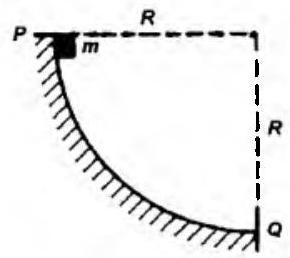
\includegraphics[width=0.4\linewidth]{images/2025_07_01_5b3ff9fa0d508c8e9f17g-004} Fig 1.1\\

1.11. O săgeată cu masa $m=60 \mathrm{~g}$ este lansată dintr-un arc cu viteza $v_{3}=40 \mathrm{~m} / \mathrm{s}$, pe verticală în sus. Accelerația gravitațională find $g=10 \mathrm{~m} / \mathrm{s}^{2}$, după un timp $t=1 \mathrm{~s}$ de la lansare, energia cinetică a săgeții este:\\ A) $25 \mathrm{~J}$; B) $27 \mathrm{~J}$; C) $30 \mathrm{~J}$; D) $40 \mathrm{~J}$; E) $17 \mathrm{~J}$; F) $1 \mathrm{~J}$.\\ (Ion M. Popescu)\\

1.12. Un corp se deplasează între punctele $x_{0}=2 \mathrm{~m}$ şi $x=22 \mathrm{~m}$. Când asupra corpului acționează forța care variază liniar cu distanța $F=60-0,5 x, x$ fiind exprimat în metri şi $F$ în Newtoni, lucrul mecanic al forței este:\\ A) $2 \mathrm{~kJ}$; B) $3 \mathrm{~kJ}$; C) $1,08 \mathrm{~kJ}$; D) $3,16 \mathrm{~kJ}$; E) $2,12 \mathrm{~kJ}$; F) $4 \mathrm{~kJ}$.\\ (Ion M. Popescu)\\

1.13. Un vagon de cale ferată cu masa $m=25 \mathrm{~t}$ ciocneşte un obstacol cu viteza $v=0,3 \mathrm{~m} / \mathrm{s}$. Resorturile celor două tampoane comprimându-se cu $x=3 \mathrm{~cm}$, forța maximă care acționează asupra fiecărui resort este (Fiecare tampon are câte un resort.):\\ A) $37 \mathrm{~kN}$; B) $38,5 \mathrm{~kN}$; C) $40 \mathrm{~kN}$; D) $20 \mathrm{~kN}$; E) $37,5 \mathrm{~kN}$; F) $1100 \mathrm{~N}$.\\ (Ion M. Popescu)\\

1.14. Un disc omogen cu raza $R=1 \mathrm{~m}$ şi masa $m=1 \mathrm{~kg}$ se roteşte în jurul axei sale fixe care trece prin centrul său cu viteza liniară $v=1 \mathrm{~m} / \mathrm{s}$. Impulsul său total este:\\ A) $2 \mathrm{~kg} \mathrm{~m} / \mathrm{s}$; B) $1 \mathrm{~kg} \mathrm{~m} / \mathrm{s}$; C) $0 \mathrm{~kg} \mathrm{~m} / \mathrm{s}$; D) $10 \mathrm{~kg} \mathrm{~m} / \mathrm{s}$; E) $40 \mathrm{~kg} \mathrm{~m} / \mathrm{s}$; F) $3 \mathrm{~kg} \mathrm{~m} / \mathrm{s}$.\\ (Ion M. Popescu)\\

1.15.* Două bile de mase $m_{1}=3 \mathrm{~kg}$ şi $m_{2}=2 \mathrm{~kg}$ se mişcă una spre cealaltă cu vitezele $v_{1}=2 \mathrm{~m} / \mathrm{s}$ şi $v_{2}=-3 \mathrm{~m} / \mathrm{s}$. În urma ciocnirii lor plastice se degajă căldura:\\ A) $10 \mathrm{~J}$; B) $9 \mathrm{~J}$; C) $5 \mathrm{~J}$; D) $16 \mathrm{~J}$; E) $15 \mathrm{~J}$; F) $26 \mathrm{~J}$.\\ (Ion M. Popescu)\\

1.16. Un automobil accelerează de la starea de repaus la viteza $v=108 \mathrm{~km} / \mathrm{h}$ in $10 \mathrm{~s}$. Forța de tractiune a motorului fiind constantă, distanța parcursă de automobil în acest timp este:\\ A) $150 \mathrm{~m}$; B) $200 \mathrm{~m}$; C) $225 \mathrm{~m}$; D) $120 \mathrm{~m}$; E) $2 \mathrm{~km}$; F) $1 \mathrm{~km}$.\\ (Constantin P. Cristescu)\\

1.17. Un corp cu masa $m=11 \mathrm{~kg}$ este tras de un resort deformat. Constanta elastică a resortului este egală cu $k=50 \mathrm{~N} / \mathrm{m}$, iar coeficientul de frecare dintre corp şi plan este $\mu=\sqrt{3} / 10$. Resortul întins face cu orizontala un unghi $\alpha=60^{\circ}$. Considerând $g=10 \mathrm{~m} / \mathrm{s}^{2}$, energia potențială minimă înmagazinată în resortul deformat necesară pentru a scoate corpul din repaus este:\\ A) $6,5 \mathrm{~J}$; B) $80 \mathrm{~J}$; C) $8,59 \mathrm{~J}$; D) $37,5 \mathrm{~J}$; E) $16 \mathrm{~J}$; F) $1,8 \mathrm{~J}$.\\ (Constantin P. Cristescu)\\

1.18. Un corp este lansat pe verticală în sus de la nivelul solului cu viteza $v_{0}$. Înălțimea față de sol la momentul în care energia cinetică este egală cu un sfert din cea potențială este:\\ A) $\frac{v_{0}^{2}}{4 g}$; B) $\frac{v_{0}^{2}}{2 g}$; C) $\frac{4 v_{0}^{2}}{15 g}$; D) $\frac{2 v_{0}^{2}}{15 g}$; E) $\frac{2 v_{0}^{2}}{5 g}$; F) $\frac{5 v_{0}^{2}}{9 g}$.\\ (Constantin P. Cristescu)\\

1.19. O macara ridică un corp cu greutatea $G=8400 \mathrm{~N}$ la o înălțime $h=35 \mathrm{~m}$ şi apoi îl deplasează orizontal pe o distanţă de $10 \mathrm{~m}$. Neglijând frecările şi considerând $g=10 \mathrm{~m} / \mathrm{s}^{2}$ lucrul efectuat de macara în această operație este:\\ A) $378 \mathrm{~kJ}$; B) $256 \mathrm{~kJ}$; C) $210 \mathrm{~kJ}$; D) $37,8 \mathrm{~kJ}$; E) $29,4 \mathrm{~kJ}$; F) $294 \mathrm{~kJ}$.\\ (Constantin P. Cristescu)\\

1.20. Un corp cu masa $m_{1}=4 \mathrm{~kg}$ agățat de un fir inextensibil este ridicat cu o accelerație $a$. Când un alt corp de masă $m_{2}=6 \mathrm{~kg}$, legat de același fir coboară cu aceeaşi accelerație $a$ (în valoare absolută) tensiunea din fir este aceeași ca în primul caz. Considerând $g=10 \mathrm{~m} / \mathrm{s}^{2}$ accelerația $a$ este:\\ A) $5 \mathrm{~m} / \mathrm{s}^{2}$; B) $2 \mathrm{~m} / \mathrm{s}^{2}$; C) $1 \mathrm{~m} / \mathrm{s}^{2}$; D) $2,5 \mathrm{~m} / \mathrm{s}^{2}$; E) $8 \mathrm{~m} / \mathrm{s}^{2}$; F) $10 \mathrm{~m} / \mathrm{s}^{2}$.\\ (Constantin P. Cristescu)\\

1.21. O forță de $5 \mathrm{~N}$ imprimă unei mase $m_{1}$ o accelerație de $a_{1}=24 \mathrm{~m} / \mathrm{s}^{2}$ și unei alte mase $m_{2}$ o accelerație de $a_{2}=8 \mathrm{~m} / \mathrm{s}^{2}$. Dacă aceeaşi forță acționează asupra ansamblului celor două corpuri, accelerația imprimată este:\\ A) $6 \mathrm{~m} / \mathrm{s}^{2}$; B) $4 \mathrm{~m} / \mathrm{s}^{2}$; C) $11 \mathrm{~m} / \mathrm{s}^{2}$; D) $14 \mathrm{~m} / \mathrm{s}^{2}$; E) $5 \mathrm{~m} / \mathrm{s}^{2}$; F) $20 \mathrm{~m} / \mathrm{s}^{2}$.\\ (Constantin P. Cristescu)\\

1.22. Asupra unui corp cu greutatea $G=20 \mathrm{~N}$ acționează simultan două forțe orizontale $F_{1}=3 \mathrm{~N}$ şi $F_{2}=4 \mathrm{~N}$ orientate pe direcții care fac un unghi de $90^{\circ}$ între ele. Considerând $g=10 \mathrm{~m} / \mathrm{s}^{2}$, accelerația cu care se mişcă corpul pe o suprafață orizontală pentru care coeficientul de frecare este de $0,25$ este:\\ A) $1 \mathrm{~m} / \mathrm{s}^{2}$; B) $0,5 \mathrm{~m} / \mathrm{s}^{2}$; C) $0 \mathrm{~m} / \mathrm{s}^{2}$; D) $0,4 \mathrm{~m} / \mathrm{s}^{2}$; E) $0,2 \mathrm{~m} / \mathrm{s}^{2}$; F) $0,35 \mathrm{~m} / \mathrm{s}^{2}$.\\ (Constantin P. Cristescu)\\

1.23. Un tren trece cu viteza $v=26 \mathrm{~m} / \mathrm{s}$ paralel cu un zid lung. Un călător din tren produce un sunet puternic şi aude ecoul (reflectat de perete) după un timp de $2 \mathrm{~s}$. Dacă sunetul se propagă cu viteza $v_{s}=340 \mathrm{~m} / \mathrm{s}$, distanţa dintre calea ferată şi zid este:\\ A) $310 \mathrm{~m}$; B) $314 \mathrm{~m}$; C) $308 \mathrm{~m}$; D) $339 \mathrm{~m}$; E) $336 \mathrm{~m}$; F) $324 \mathrm{~m}$.\\ (Constantin P. Cristescu)\\

1.24. Un automobil urcă o pantă cu $\alpha=\left(\frac{9}{\pi}\right)$ grade fără motor, viteza sa inițială la baza pantei fiind de $v_{0}=72 \mathrm{~km} / \mathrm{h}$. Considerând $g=10 \mathrm{~m} / \mathrm{s}^{2}$, facând aproximația $\sin \alpha=\alpha rad$ şi neglijând frecările, timpul în care viteza automobilului se reduce la $v=18 \mathrm{~km} / \mathrm{h}$ este:\\ A) $20 \mathrm{~s}$; B) $30 \mathrm{~s}$; C) $40 \mathrm{~s}$; D) $25 \mathrm{~s}$; E) $34 \mathrm{~s}$; F) $18 \mathrm{~s}$.\\ (Constantin P. Cristescu)\\

1.25. Un corp de dimensiuni mici este aruncat de la nivelul solului pe verticală în sus. Dacă el se află în aer timp de $4 \mathrm{~s}$, aproximând $g=10 \mathrm{~m} / \mathrm{s}^{2}$, înălțimea maximă atinsă de corp este:\\ A) $20 \mathrm{~m}$; B) $18 \mathrm{~m}$; C) $24 \mathrm{~m}$; D) $15 \mathrm{~m}$; E) $45 \mathrm{~m}$; F) $30 \mathrm{~m}$.\\ (Constantin P. Cristescu)\\

1.26. Un corp lansat pe o suprafaţă orizontală cu viteza inițială $v_{0}=20 \mathrm{~m} / \mathrm{s}$ parcurge în secunda a cincea distanţa de $5 \mathrm{~m}$. Considerând $g=10 \mathrm{~m} / \mathrm{s}^{2}$, coeficientul de frecare este:\\ A) $0,4$; B) $0,08$; C) $1 / 3$; D) $\sqrt{3} / 6$; E) $0,2 / 3$; F) $1 / 6$.\\ (Constantin P. Cristescu)\\

1.27.* Un vagon de tren cu masa $m_{1}=21 \mathrm{~t}$ şi cu viteza de $v_{1}=6 \mathrm{~m} / \mathrm{s}$ ciocneşte un alt vagon cu masa $m_{2}=49 \mathrm{t}$ care se mişcă în acelaşi sens cu viteza de $v_{2}=3 \mathrm{~m} / \mathrm{s}$, astfel încât după ciocnire ele se mişcă împreună. Viteza ansamblului celor două vagoane este:\\ A) $5 \mathrm{~m} / \mathrm{s}$; B) $4,8 \mathrm{~m} / \mathrm{s}$; C) $3,2 \mathrm{~m} / \mathrm{s}$; D) $4,1 \mathrm{~m} / \mathrm{s}$; E) $3,9 \mathrm{~m} / \mathrm{s}$; F) $4,5 \mathrm{~m} / \mathrm{s}$.\\ (Constantin P. Cristescu)\\

1.28. Un avion care zboară cu viteza constantă $v=360 \mathrm{~km} / \mathrm{h}$, descrie o buclă circulară în plan vertical. Considerând $g=10 \mathrm{~m} / \mathrm{s}^{2}$, raza maximă posibilă a buclei este:\\ A) $1 \mathrm{~km}$; B) $2 \mathrm{~km}$; C) $800 \mathrm{~m}$; D) $1,6 \mathrm{~km}$; E) $500 \mathrm{~m}$; F) $1250 \mathrm{~m}$.\\ (Constantin P. Cristescu)\\

1.29. Un automobil se deplasează pe un pod convex de forma unui arc de cerc cu raza $r=22,5 \mathrm{~m}$. Considerând $g=10 \mathrm{~m} / \mathrm{s}^{2}$, viteza maximă pentru care automobilul rămâne în contact cu podul în punctul cel mai de sus este:\\ A) $120 \mathrm{~km} / \mathrm{h}$; B) $72 \mathrm{~km} / \mathrm{h}$; C) $20 \mathrm{~m} / \mathrm{s}$; D) $17 \mathrm{~m} / \mathrm{s}$; E) $15 \mathrm{~m} / \mathrm{s}$; F) $30 \mathrm{~m} / \mathrm{s}$.\\ (Constantin P. Cristescu)\\

1.30.* Două sfere de mase $m_{1}$ şi $m_{2}$ având viteze egale şi orientate în sens opus se ciocnesc perfect elastic. După ciocnire, sfera de masă $m_{1}$ rămâne în repaus. Raportul maselor celor două sfere $m_{1} / m_{2}$ este:\\ A) $1 / 2$; B) $3$; C) $2$; D) $4,5$; E) $0,8$; F) $5$.\\ (Constantin P. Cristescu)\\

1.31. Un corp cu masa $m=1 \mathrm{~kg}$ legat cu o sârmă cu lungimea $l_{0}=1 \mathrm{~m}$ este rotit astfel încât descrie o traiectorie aproximativ circulară în plan vertical. Viteza constantă a corpului este astfel încât forța centrifugă este dublul greutății corpului. Modulul de elasticitate al sârmei este $E=10^{11} \mathrm{~N} / \mathrm{m}^{2}$, iar secțiunea sa este $S=0,5 \cdot 10^{-6} \mathrm{~m}^{2}$. În cursul mişcării lungimea sârmei variază în intervalul:\\ A) $(100,02 \div 100,06) \mathrm{cm}$; B) $(100,10 \div 100,30) \mathrm{cm}$; C) $(100,01 \div 100,05) \mathrm{cm}$; D) $(100,05 \div 100,10) \mathrm{cm}$; E) $(100,04 \div 100,09) \mathrm{cm}$; F) $(100,03 \div 100,06) \mathrm{cm}$.\\ (Constantin P. Cristescu)\\

1.32. Două corpuri cu masele $m_{1}$ şi $m_{2}$ sunt legate unul de altul cu un fir de masă neglijabilă. Asupra corpului de masă $m_{1}$ acționează o forță orizontală $F$, iar coeficientul de frecare dintre corpuri şi suprafața orizontală pe care se află este $\mu$. Tensiunea din firul de legătură este:\\ A) $\frac{F m_{1}}{m_{1}+m_{2}}$; B) $\frac{F m_{2}}{m_{1}+m_{2}}$; C) $\frac{F m_{1} m_{2}}{\left(m_{1}+m_{2}\right)^{2}}$; D) $F-\mu m_{2} g$; E) $\frac{F\left(m_{1}+m_{2}\right)}{m_{2}}$; F) $F-\mu\left(m_{1}+m_{2}\right) g$.\\ (Constantin P. Cristescu)\\

1.33. Un corp este lansat de jos în sus pe un plan înclinat de unghi $\alpha=30^{\circ}$. Dacã timpul de coborâre este de $n=4$ ori mai mare decât cel de urcare, coeficientul de frecare dintre corp şi plan este:\\ A) $\frac{\sqrt{3}}{10}$; B) $\frac{2 \sqrt{3}}{15}$; C) $\frac{\sqrt{3}}{8}$; D) $\frac{\sqrt{3}}{12}$; E) $\frac{5 \sqrt{3}}{17}$; F) $\frac{3 \sqrt{3}}{10}$.\\ (Constantin P. Cristescu)\\

1.34. Mişcarea unui corp este descrisă de ecuația $x=8+20 t-2 t^{2}$ unde $x$ este în metri şi $t$ este în secunde. Viteza corpului la momentul $t=2,3 \mathrm{~s}$ este:\\ A) $10,7 \mathrm{~m} / \mathrm{s}$; B) $15 \mathrm{~m} / \mathrm{s}$; C) $8,8 \mathrm{~m} / \mathrm{s}$; D) $18 \mathrm{~m} / \mathrm{s}$; E) $11,2 \mathrm{~mm} / \mathrm{s}$; F) $10,8 \mathrm{~m} / \mathrm{s}$.\\ (Constantin P. Cristescu)\\

1.35. Ecuația vitezei unui corp este $v=12-t$ unde $v$ este măsurat în $\mathrm{m} / \mathrm{s}$, iar $t$ în secunde. Dacă inițial $(t=0)$ coordonata de poziție a corpului este $x_{0}=10 \mathrm{~m}$, coodonata la momentul $t=8 \mathrm{~s}$ este:\\ A) $74 \mathrm{~m}$; B) $16 \mathrm{~m}$; C) $32 \mathrm{~m}$; D) $124 \mathrm{~m}$; E) $65 \mathrm{~m}$; F) $108 \mathrm{~m}$.\\ (Constantin P. Cristescu)\\

1.36. Un corp cu masa $m=4,2 \mathrm{~kg}$ este lansat în jos pe un plan înclinat cu unghiul $\alpha$ dat de $\operatorname{tg} \alpha=\mu, \mu$ find coeficientul de frecare. Dacă înălțimea inițială a corpului față de baza planului este $h=2,5 \mathrm{~m}$ şi se consideră $g=10 \mathrm{~m} / \mathrm{s}^{2}$, lucrul mecanic consumat prin frecare de-a lungul planului este:\\ A) $230 \mathrm{~J}$; B) $175 \mathrm{~J}$; C) $105 \mathrm{~J}$; D) $208 \mathrm{~J}$; E) $244 \mathrm{~J}$; F) $98 \mathrm{~J}$.\\ (Constantin P. Cristescu)\\

1.37. Un corp aflat la o înălțime oarecare este aruncat în direcție orizontală cu viteza $v_{0}$. Graficul vitezei corpului ca funcție de timp are forma:\\ A) 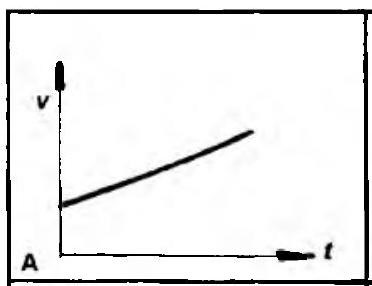
\includegraphics[width=0.4\linewidth]{images/2025_07_01_5b3ff9fa0d508c8e9f17g-010(2)A}; B) 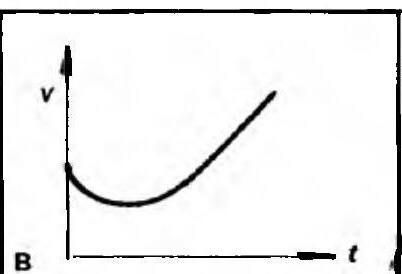
\includegraphics[width=0.4\linewidth]{images/2025_07_01_5b3ff9fa0d508c8e9f17g-010(2)B}; C) 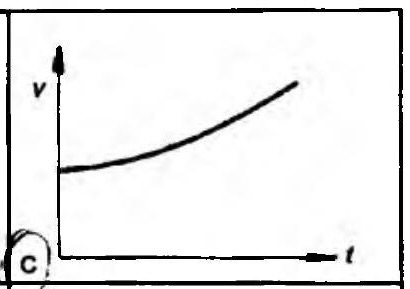
\includegraphics[width=0.4\linewidth]{images/2025_07_01_5b3ff9fa0d508c8e9f17g-010(2)C}; D) 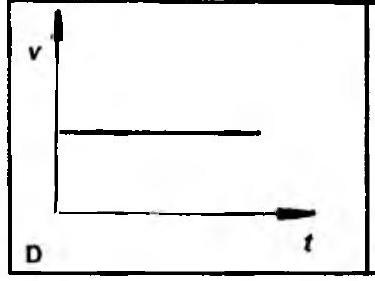
\includegraphics[width=0.4\linewidth]{images/2025_07_01_5b3ff9fa0d508c8e9f17g-010(2)D}; E) 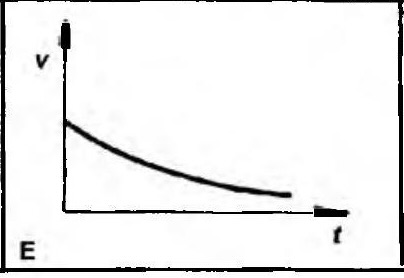
\includegraphics[width=0.4\linewidth]{images/2025_07_01_5b3ff9fa0d508c8e9f17g-010(2)E}; F) 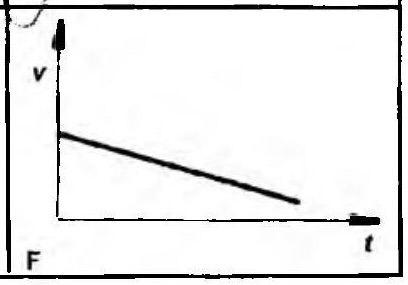
\includegraphics[width=0.4\linewidth]{images/2025_07_01_5b3ff9fa0d508c8e9f17g-010(2)F}.\\ (Alexandru M. Preda)\\

1.38. Cu o armă având lungimea țevii $l=25 \mathrm{~cm}$ şi secțiunea interioară $A=80 \mathrm{~mm}^{2}$ se trage un glonț cu masa $m=50 \mathrm{~g}$. Dacă glonțul parcurge lungimea țevii sub acțiunea unei presiuni constante $p=2 \cdot 10^{8} \mathrm{~N} / \mathrm{m}^{2}$ şi considerând frecarea neglijabilă, viteza glonțului la ieşirea din țeavă este:\\ A) $55 \mathrm{~m} / \mathrm{s}$; B) $400 \mathrm{~m} / \mathrm{s}$; C) $500 \mathrm{~m} / \mathrm{s}$; D) $375 \mathrm{~m} / \mathrm{s}$; E) $440 \mathrm{~m} / \mathrm{s}$; F) $620 \mathrm{~m} / \mathrm{s}$.\\ (Alexandru M. Preda)\\

1.39. Asupra unui corp cu masa $m=3 \mathrm{~kg}$ aflat pe o suprafață pe care se poate mişca fară frecare, acționează o forţă care depinde de timp conform graficului din Fig.1.2. Cunoscând că $v_{0}=0$, la sfârşitul celei de a 5-a secunde viteza corpului este:\\ A) $11 \mathrm{~m} / \mathrm{s}$; B) $10 \mathrm{~m} / \mathrm{s}$; C) $12,5 \mathrm{~m} / \mathrm{s}$; D) $12 \mathrm{~m} / \mathrm{s}$; E) $14 \mathrm{~m} / \mathrm{s}$; F) $9,5 \mathrm{~m} / \mathrm{s}$.\\ (Alexandru M. Preda)\\ 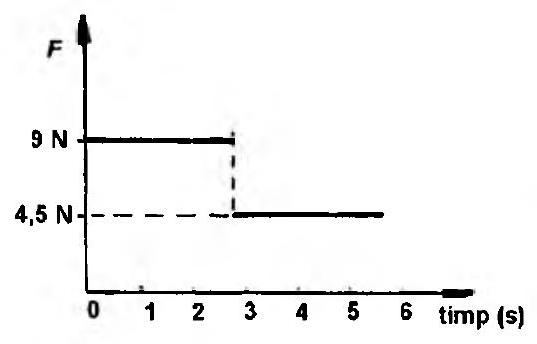
\includegraphics[width=0.4\linewidth]{images/2025_07_01_5b3ff9fa0d508c8e9f17g-010(1)} Fig. 1.2\\ 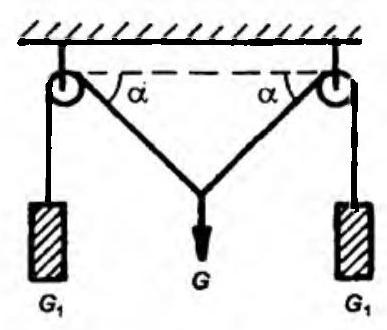
\includegraphics[width=0.4\linewidth]{images/2025_07_01_5b3ff9fa0d508c8e9f17g-010} Fig. 1.3\\

1.40. Un corp de greutate $G$ este suspendat ca în Fig. 1.3. Care dintre graficele de mai jos reprezintă dependenta de unghiul $\alpha$ a greutății $G_{1}$ care asigură echilibrul sistemului?\\ A) 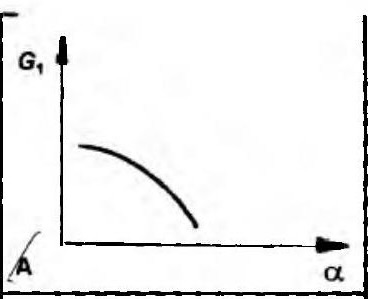
\includegraphics[width=0.4\linewidth]{images/2025_07_01_5b3ff9fa0d508c8e9f17g-011(2)A}; B) 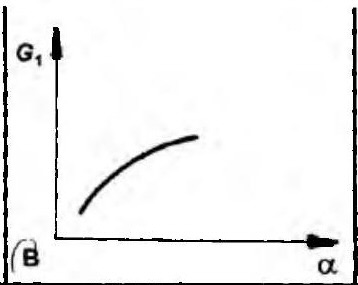
\includegraphics[width=0.4\linewidth]{images/2025_07_01_5b3ff9fa0d508c8e9f17g-011(2)B}; C) 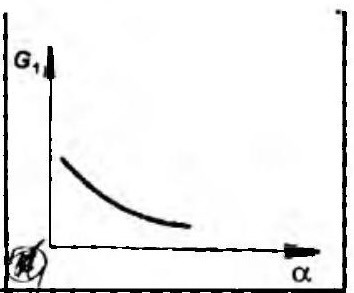
\includegraphics[width=0.4\linewidth]{images/2025_07_01_5b3ff9fa0d508c8e9f17g-011(2)C}; D) 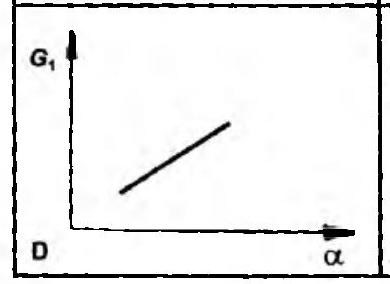
\includegraphics[width=0.4\linewidth]{images/2025_07_01_5b3ff9fa0d508c8e9f17g-011(2)D}; E) 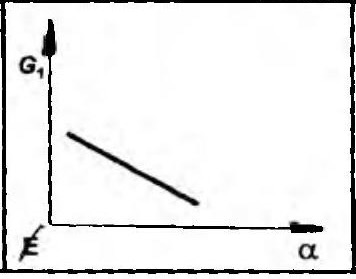
\includegraphics[width=0.4\linewidth]{images/2025_07_01_5b3ff9fa0d508c8e9f17g-011(2)E}; F) 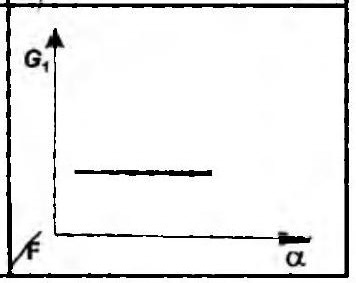
\includegraphics[width=0.4\linewidth]{images/2025_07_01_5b3ff9fa0d508c8e9f17g-011(2)F}.\\ (Alexandru M. Preda)\\ 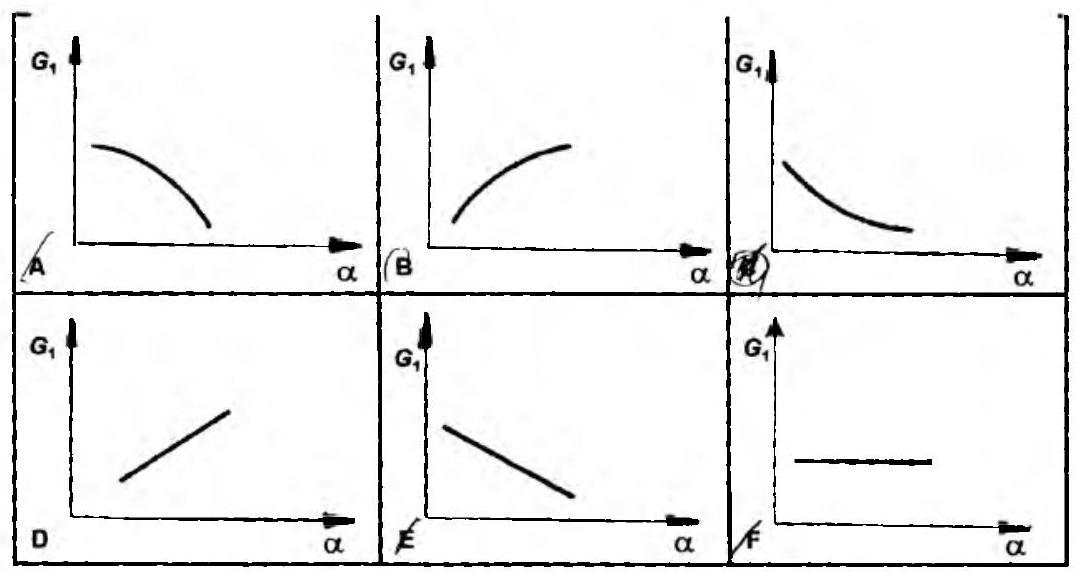
\includegraphics[width=0.4\linewidth]{images/2025_07_01_5b3ff9fa0d508c8e9f17g-011(2)} Fig. 1.3.\\

1.41. Un automobil cu masa $m=800 \mathrm{~kg}$ se deplasează cu viteza $v_{0}=10 \mathrm{~m} / \mathrm{s}$. Şoferul observă un obstacol aflat în față la distanță $d=6,4 \mathrm{~m}$ de autombil și acționează frâna. Ştiind că forța de frânare asigură oprirea completă pe o distanță de $10 \mathrm{~m}$, impulsul pe care îl transferă automobilul obstacolului la ciocnire este:\\ A) $2300 \mathrm{~kg} \mathrm{~m} / \mathrm{s}$; B) $4800 \mathrm{~kg} \mathrm{~m} / \mathrm{s}$; C) $5200 \mathrm{~kg} \mathrm{~m} / \mathrm{s}$; D) $6350 \mathrm{~kg} \mathrm{~m} / \mathrm{s}$; E) $3850 \mathrm{~kg} \mathrm{~m} / \mathrm{s}$; F) $5000 \mathrm{~kg} \mathrm{~m} / \mathrm{s}$.\\ (Alexandru M. Preda)\\

1.42. Care dintre graficele de mai jos corespunde dependenţei de timp a vitezei unei bile aruncate vertical în sus şi care în cădere suferă ciocniri perfect elastice și instantanee cu o suprafață plană orizontală? Momentul inițial este momentul aruncării.\\ A) 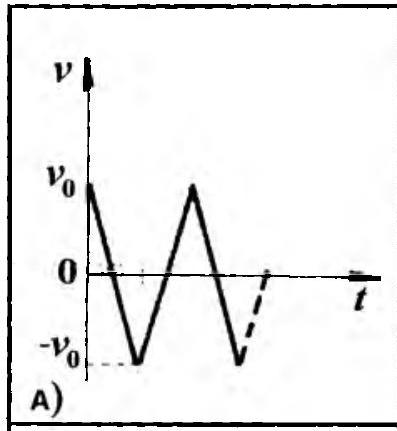
\includegraphics[width=0.4\linewidth]{images/2025_07_01_5b3ff9fa0d508c8e9f17g-011}; B) 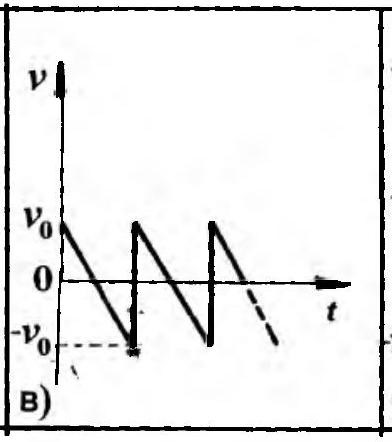
\includegraphics[width=0.4\linewidth]{images/2025_07_01_5b3ff9fa0d508c8e9f17g-011(1)B}; C) 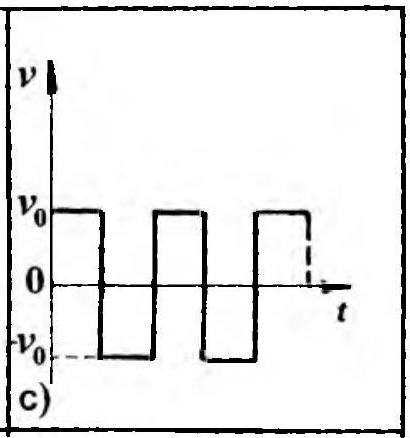
\includegraphics[width=0.4\linewidth]{images/2025_07_01_5b3ff9fa0d508c8e9f17g-011(1)C}; D) 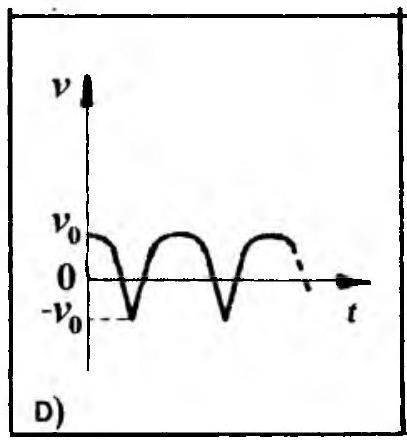
\includegraphics[width=0.4\linewidth]{images/2025_07_01_5b3ff9fa0d508c8e9f17g-012(1)D}; E) 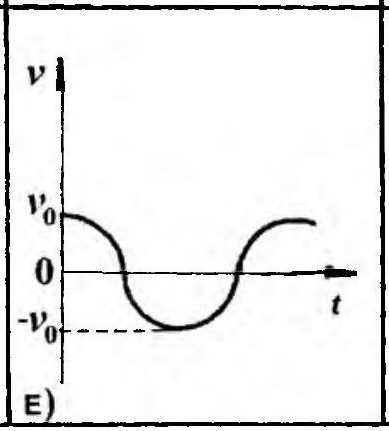
\includegraphics[width=0.4\linewidth]{images/2025_07_01_5b3ff9fa0d508c8e9f17g-012(1)E}; F) 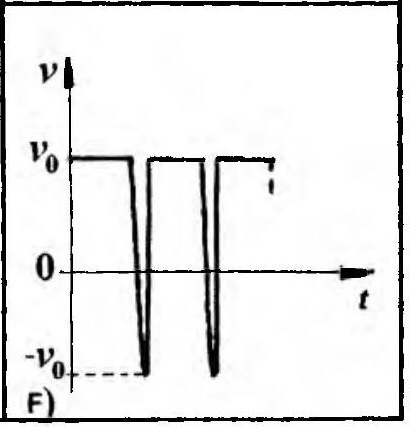
\includegraphics[width=0.4\linewidth]{images/2025_07_01_5b3ff9fa0d508c8e9f17g-012(1)F}.\\ (Alexandru M. Preda)\\

1.43. Un corp cade liber de la o înățime $h$. După un interval de timp $\tau$ de la pornirea primului corp, cade liber de la aceeaşi înălțime, un al doilea corp. Ce fel de mişcare execută primul corp față de al doilea corp?\\ A) Uniform accelerată cu $a=g$; B) Uniform acceleratã cu $a=g / 2$; C) Uniform accelerată cu $a=2 g$; D) Uniformă; E) Accelerată cu accelerație variabilă; F) Uniform încetinită cu acceleraţia $a=g / 2$.\\ (Maria Honciuc)\\

1.44. Un mobil se mişcă uniform cu viteza $v_{1}=5 \mathrm{~m} / \mathrm{s}$. La un moment dat, un alt mobil care vine din acelaşi sens, aflat la distanța $d$ de primul, începe să frâneze de la viteza $v_{2}=10 \mathrm{~m} / \mathrm{s}$. Acceleraţia de frânare este $a=0,1 \mathrm{~m} / \mathrm{s}^{2}$. Care este spațiul parcurs de primul mobil, până la prima intâlnire a mobilelor? (Mobilele se întâlnesc o singură dată).\\ A) $250 \mathrm{~m}$; B) $125 \mathrm{~m}$; C) $500 \mathrm{~m}$; D) $175 \mathrm{~m}$; E) $300 \mathrm{~m}$; F) $50 \mathrm{~m}$.\\ (Maria Honciuc)\\

1.45. Fie sistemul format din masele $m_{1}$ şi $m_{2}=3 m_{1}$ care sunt legate printr-un fir inextensibil, de greutate neglijabilă, trecut peste un scripete, ca în Fig. 1.4. Se cunoaşte coeficientul de frecare pe planul orizontal $\mu=0,15$. Sistemul se mişcă cu accelerația $a_{1}$. Dacă schimbăm locul corpurilor între ele, sistemul se mişcă cu accelerația $a_{2}$. Găsiți care este relația dintre accelerații:\\ A) $a_{1}=2,5 a_{2}$; B) $a_{1}=3 a_{2}$; C) $a_{1}=3,5 a_{2}$; D) $a_{1}=5,18 a_{2}$; E) $a_{1}=3,15 a_{2}$; F) $a_{1}=5,7 a_{2}$.\\ (Maria Honciuc)\\ 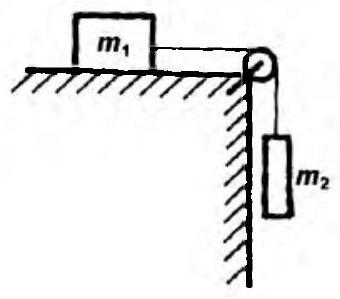
\includegraphics[width=0.4\linewidth]{images/2025_07_01_5b3ff9fa0d508c8e9f17g-012} Fig. 1.4\\

1.46. Doi pietoni aflați în localitățile A şi B pornesc unul spre altul în acelaşi moment, într-o mişcare rectilinie uniformă. În momentul întâlnirii, primul parcursese cu $1,5 \mathrm{~km}$ mai mult decât celălalt. După întâlnire, pietonii își continuă drumul. Primul ajunge în localitatea B după un timp $t_{1}$ de la intâlnire, iar al doilea ajunge în localitatea A dupã un timp $t_{2}$. Dacă $t_{1}=30$ minute şi $t_{2}=1$ oră, vitezele cu care se mişcă cei doi pietoni sunt:\\ A) $v_{1}=2 \mathrm{~m} / \mathrm{s}, v_{2}=1,42 \mathrm{~m} / \mathrm{s}$; B) $v_{1}=7,2 \mathrm{~km} / \mathrm{h}, v_{2}=10 \mathrm{~km} / \mathrm{h}$; C) $v_{1}=7,2 \mathrm{~km} / \mathrm{h}, v_{2}=5,5 \mathrm{~km} / \mathrm{h}$; D) $v_{2}=3 \mathrm{~m} / \mathrm{s}, v_{2}=5 \mathrm{~km} / \mathrm{h}$; E) $v_{1}=7,2 \mathrm{~km} / \mathrm{h}, v_{2}=1,5 \mathrm{~m} / \mathrm{s}$; F) $v_{1}=5 \mathrm{~m} / \mathrm{s}, v_{2}=7,2 \mathrm{~m} / \mathrm{s}$.\\ (Maria Honciuc)\\

1.47. Un corp este menținut în echilibru pe un plan înclinat de unghi $\alpha$ față de orizontală, fie cu o forță minimă orizontală, fie cu o forță minimă normală pe plan de $k$ ori mai mare decât prima. Coeficientul de frecare dintre corp și plan este:\\ A) $\mu=\frac{\sin \alpha}{k-\sin \alpha}$; B) $\mu=\frac{\cos \alpha}{k+\sin \alpha}$; C) $\mu=\frac{\cos \alpha}{k-\sin \alpha}$; D) $\mu=\frac{k}{k-\sin \alpha}$; E) $\mu=\frac{\cos ^{2} \alpha}{k-\sin \alpha}$; F) $\mu=\frac{\cos \alpha}{k \cos \alpha-\sin \alpha}$.\\ (Maria Honciuc)\\

1.48. Un corp este lansat în sus, pe un plan înclinat de unghi $\alpha=30^{\circ}$ cu orizonatala şi apoi revine la baza planului. Dacă timpul de urcare este de $k=1,1$ ori mai mic decât timpul de coborâre, coeficientul de frecare dintre corp şi planul înclinat este:\\ A) $\mu=0,5$; B) $\mu=0,8$; C) $\mu=0,25$; D) $\mu=0,45$; E) $\mu=0,055$; F) $\mu=0,455$.\\ (Maria Honciuc)\\

1.49. Un mobil este aruncat cu viteza inițială $v_{0}$, pe verticală, în sus. Momentele de timp la care energia cinetică a corpului este egală cu energia potențială sunt:\\ A) $t_{1,2}=\frac{2 v_{0} \pm \sqrt{2}}{2 g}$; B) $t_{1,2}=\frac{v_{0}(2 \pm \sqrt{2})}{g}$; C) $t_{1,2}=\frac{v_{0}(2 \pm \sqrt{2})}{2}$; D) $t_{1,2}=\frac{v_{0}(2 \mp \sqrt{3})}{2 g}$; E) $t_{1,2}=\frac{v_{0}(1 \pm \sqrt{2})}{2 g}$; F) $t_{1,2}=\frac{v_{0}(2 \pm \sqrt{2})}{2 g}$.\\ (Maria Honciuc)\\

1.50.* Acele unui ceasornic indică ora 12. Să se determine timpul după care orarul şi minutarul sunt prima dată perpendiculare, respectiv din nou suprapuse.\\ A) $t_{1}=1,63 \mathrm{~min}, t_{2}=1,09 \mathrm{~min}$; B) $t_{1}=900 \mathrm{~s}, t_{2}=1,09 \mathrm{~h}$; C) $t_{1}=16,36 \mathrm{~min}, t_{2}=65,45 \mathrm{~min}$; D) $t_{1}=981,6 \mathrm{~s}, t_{2}=300 \mathrm{~min}$; E) $t_{1}=900 \mathrm{~s}, t_{2}=65 \mathrm{~min}$; F) $t_{1}=16,36 \mathrm{~min}, t_{2}=6,55 \mathrm{~min}$.\\ (Maria Honciuc)\\

1.51. Un corp cade liber de la înălțimea $h$, iar altul este lansat simultan pe vertícală de la suprafața Pământului. Ce înălțime maximă va atinge al doilea mobil, știind că ambele corpuri ating simultan solul.\\ A) $h$; B) $h / 2$; C) $h / 4$; D) $2 h$; E) $\sqrt{h}$; F) $h / 3$.\\ (Corneliu Ghizdeanu)\\

1.52. O minge este lansată pe verticală de la sol cu viteza inițială $v_{0}=40 \mathrm{~m} / \mathrm{s}$. Se cere înălțimea maximă la care ajunge mingea după ciocnirea cu solul, dacă sărind pierde instantaneu jumătate din energia pe care o posedă în momentul atingerii solului ($g=10 \mathrm{~m} / \mathrm{s}^{2}$).\\ A) $80 \mathrm{~m}$; B) $60 \mathrm{~m}$; C) $40 \mathrm{~m}$; D) $20 \mathrm{~m}$; E) $40 \sqrt{2} \mathrm{~m}$; F) $55 \mathrm{~m}$.\\ (Corneliu Ghizdeanu)\\

1.53. Din acelaşi punct, aflat la înălțimea $h_{0}=245 \mathrm{~m}$ deasupra solului, sunt lăsate să cadă liber, la un interval de timp $\Delta t=2 \mathrm{~s}$, două corpuri. Se cere distanța maximă dintre corpurile aflate încă în aer ($g=10 \mathrm{~m} / \mathrm{s}^{2}$).\\ A) $200 \mathrm{~m}$; B) $120 \mathrm{~m}$; C) $24,5 \mathrm{~m}$; D) $140 \mathrm{~m}$; E) $150 \mathrm{~m}$; F) $145 \mathrm{~m}$.\\ (Corneliu Ghizdeanu)\\

1.54. O bilă este atârnată de un fir subțire de lungime $l=0,2 \mathrm{~m}$ şi scoasă succesiv din poziția de echilibru cu unghiurile $\alpha_{1}=45^{\circ}$, respectiv $\alpha_{2}=30^{\circ}$ şi apoi este lăsată liberă. Se cere raportul vitezelor cu care bila trece prin poziția de echilibru pentru cele două situații ($g=10 \mathrm{~m} / \mathrm{s}^{2}$).\\ A) $1$; B) $2$; C) $2,45$; D) $1,478$; E) $0,5$; F) $1,25$.\\ (Corneliu Ghizdeanu)\\

1.55. Un glonte pătrunde într-o scândură pe o distanță $d$ având o viteză inițială $v_{0}=200 \mathrm{~m} / \mathrm{s}$. Să se calculeze viteza $v$ cu care iese glontele dintr-o scândură din acelaşi material, care are grosimea pe jumătate.\\ A) $200 \mathrm{~m} / \mathrm{s}$; B) $150 \mathrm{~m} / \mathrm{s}$; C) $125,5 \mathrm{~m} / \mathrm{s}$; D) $141 \mathrm{~m} / \mathrm{s}$; E) $98 \mathrm{~m} / \mathrm{s}$; F) $140 \mathrm{~m} / \mathrm{s}$.\\ (Corneliu Ghizdeanu)\\

1.56. Un tren cu masa totală $m=200 \mathrm{t}$ este tras pe o linie orizontală de o locomotivă cu puterea $P=400 \mathrm{~kW}$. Coeficientul de frecare dintre tren şi şine este $\mu=0,01$. Se cere accelerația sa în momentul când viteza are valoarea $v=2 \mathrm{~m} / \mathrm{s}$ cât şi valoarea vitezei maxime ($g=10 \mathrm{~m} / \mathrm{s}^{2}$).\\ A) $1,9 \mathrm{~m} / \mathrm{s}^{2}, 10 \mathrm{~m} / \mathrm{s}$; B) $2 \mathrm{~m} / \mathrm{s}^{2}, 10 \mathrm{~m} / \mathrm{s}$; C) $0,9 \mathrm{~m} / \mathrm{s}^{2}, 20 \mathrm{~m} / \mathrm{s}$; D) $1,9 \mathrm{~m} / \mathrm{s}^{2}, 20 \mathrm{~m} / \mathrm{s}$; E) $0,9 \mathrm{~m} / \mathrm{s}^{2}, 40 \mathrm{~m} / \mathrm{s}$; F) $0,5 \mathrm{~m} / \mathrm{s}^{2}, 20 \mathrm{~m} / \mathrm{s}$.\\ (Corneliu Ghizdeanu)\\

1.57.* Pentru un pendul conic se cunosc: $l, \alpha, g$. Perioada lui de rotație este:\\ A) $2\pi \lfloor \sqrt{l \cos \alpha / g} \rfloor$; B) $2\pi \lfloor \sqrt{l / g} \rfloor$; C) $2\pi \lfloor \sqrt{l \sin \alpha / g} \rfloor$; D) $2\pi \lfloor \sqrt{l \tan \alpha / g} \rfloor$; E) $2\pi \lfloor \sqrt{m / (l \cos \alpha \cdot g)} \rfloor$; F) $2\pi \lfloor \sqrt{m / (l \sin \alpha \cdot g)} \rfloor$.\\ (Corneliu Ghizdeanu)\\

1.58. Un corp cu $m=1 \mathrm{~kg}$ se mişcă uniform accelerat fară viteză inițială parcurgând în prima secundă $0,5 \mathrm{~m}$. Cât este energia cinetică a corpului după $2 \mathrm{~s}$?\\ A) $2 \mathrm{~J}$; B) $10 \mathrm{~J}$; C) $0,1 \mathrm{~J}$; D) $20 \mathrm{~J}$; E) $0,2 \mathrm{~J}$; F) $0,01 \mathrm{~J}$.\\ (Niculae N. Puşcaş)\\

1.59. Un corp se mişcă uniform accelerat parcurgând în prima secundă $1 \mathrm{~m}$, iar în a doua secundă $2 \mathrm{~m}$. Cât este accelerația corpului?\\ A) $10 \mathrm{~m} / \mathrm{s}^{2}$; B) $5 \mathrm{~m} / \mathrm{s}^{2}$; C) $0,1 \mathrm{~m} / \mathrm{s}^{2}$; D) $4 \mathrm{~m} / \mathrm{s}^{2}$; E) $0,01 \mathrm{~m} / \mathrm{s}^{2}$; F) $1 \mathrm{~m} / \mathrm{s}^{2}$.\\ (Niculae N. Puşcaş)\\

1.60. Două corpuri având masele $200 \mathrm{~g}$, respectiv $300 \mathrm{~g}$ sunt legate cu un fir care este trecut peste un scripete fix. După cât timp distanța dintre corpuri devine $2 \mathrm{~m}? (g=10 \mathrm{~m} / \mathrm{s}^{2})$\\ A) $0,1 \mathrm{~s}$; B) $5 \mathrm{~s}$; C) $10 \mathrm{~s}$; D) $4 \mathrm{~s}$; E) $1 \mathrm{~s}$; F) $0,01 \mathrm{~s}$.\\ (Niculae N. Puşcaş)\\

1.61.* Un corp cu masa de $1 \mathrm{~kg}$ este aruncat de jos în sus cu viteza de $80 \mathrm{~m} / \mathrm{s}$, iar altul identic în jos de la înălțimea de $100 \mathrm{~m}$ cu viteza inițială de $20 \mathrm{~m} / \mathrm{s}$. Cât este energia cinetică a corpului rezultat în urma ciocnirii plastice? ($g=10 \mathrm{~m} / \mathrm{s}^{2}$)\\ A) $40 \mathrm{~J}$; B) $400 \mathrm{~J}$; C) $100 \mathrm{~J}$; D) $1000 \mathrm{~J}$; E) $10 \mathrm{~J}$; F) $1 \mathrm{~J}$.\\ (Niculae N. Puşcaş)\\

1.62. Un automobil cu puterea de $30 \mathrm{~kW}$ se deplasează uniform accelerat pe o şosea orizontală. Cât este spațiul parcurs între două momente de timp în care viteza automobilului este $5 \mathrm{~m} / \mathrm{s}$, respectiv $20 \mathrm{~m} / \mathrm{s}$, ştiind că a fost efectuat un lucru mecanic de $0,3 \mathrm{~MJ}$?\\ A) $125 \mathrm{~m}$; B) $500,5 \mathrm{~m}$; C) $10 \mathrm{~m}$; D) $1000 \mathrm{~m}$; E) $50 \mathrm{~m}$; F) $2000 \mathrm{~m}$.\\ (Niculae N. Puşcaş)\\

1.63. Un corp este aşezat pe un plan înclinat de unghi $\alpha (\operatorname{tg} \alpha=1)$. Planul este împins cu accelerația orizontală de $15 \mathrm{~m} / \mathrm{s}^{2}$, iar corpul începe sã urce pe plan. Cât este coeficientul de frecare dintre corp şi planul înclinat? ($g=10 \mathrm{~m} / \mathrm{s}^{2}$)\\ A) $0,01$; B) $0,2$; C) $1$; D) $0,9$; E) $0,02$; F) $0,6$.\\ (Niculae N. Puşcaş)\\

1.64. În cât timp un tren având masa de $10^{6} \mathrm{~kg}$ care pleacă din repaus pe un drum orizontal, ajunge la viteza de $20 \mathrm{~m} / \mathrm{s}$, ştiind că forţa de tracțiune a locomotivei este de $0,5 \mathrm{MN}$, iar coeficientul de frecare dintre şine şi roţi este 0,03? ($g=10 \mathrm{~m} / \mathrm{s}^{2}$)\\ A) $10 \mathrm{~s}$; B) $20 \mathrm{~s}$; C) $100 \mathrm{~s}$; D) $200 \mathrm{~s}$; E) $15 \mathrm{~s}$; F) $5 \mathrm{~min}$.\\ (Niculae N. Puşcaş)\\

1.65.* Cât este viteza unui proiectil cu masa de $0,5 \mathrm{~kg}$, care ciocnind plastic un corp cu masa de $99,5 \mathrm{~kg}$, suspendat de un fir de $0,5 \mathrm{~m}$, determină rotația în plan vertical a sistemului proiectil + corp, firul fiind întins? ($g=10 \mathrm{~m} / \mathrm{s}^{2}$)\\ A) $100 \mathrm{~m} / \mathrm{s}$; B) $11000 \mathrm{~m} / \mathrm{s}$; C) $20 \mathrm{~m} / \mathrm{s}$; D) $1000 \mathrm{~m} / \mathrm{s}$; E) $300 \mathrm{~m} / \mathrm{s}$; F) $1 \mathrm{~m} / \mathrm{s}$.\\ (Niculae N. Puşcaş)\\

1.66. Asupra unui corp acționează o forță care variază direct proporțional cu distanța. Ştiind că la distanța $x_{1}=1 \mathrm{~m}$ față de origine forța este $10 \mathrm{~N}$, cât este lucrul mecanic efectuat de forţă când este deplasat între punctele $x_{1}=1 \mathrm{~m}$ şi $x_{2}=2 \mathrm{~m}$ ?\\ A) $1 \mathrm{~J}$; B) $50 \mathrm{~J}$; C) $100 \mathrm{~J}$; D) $0,1 \mathrm{~J}$; E) $15 \mathrm{~J}$; F) $200 \mathrm{~J}$.\\ (Niculae N. Puşcaş)\\

1.67. Un corp cu masa de $2 \mathrm{~kg}$ este suspendat de tavan prin intermediul a trei fire, ca în Fig. 1.5. Unghiurile $\alpha_{1}$ şi $\alpha_{2}$ au valorile: $\alpha_{1}=30^{\circ}, \alpha_{2}=60^{\circ}$. Să se determine valoarea forțelor de tensiune în cele trei fire. ($g=9,8 \mathrm{~m} / \mathrm{s}^{2}$)\\ A) $T=19,6 \mathrm{~N}, T_{1}=9,8 \mathrm{~N}, T_{2}=9,8 \sqrt{3} \mathrm{~N}$; B) $T=19,6 \mathrm{~N}, T_{1}=9,8 \sqrt{3} \mathrm{~N}, T_{2}=9,8 \sqrt{3} \mathrm{~N}$; C) $T=39,2 \mathrm{~N}, T_{1}=9,8 \mathrm{~N}, T_{2}=9,8 \mathrm{~N}$; D) $T=19,6 \sqrt{3} \mathrm{~N}, T_{1}=9,8 \mathrm{~N}, T_{2}=9,8 \sqrt{3} \mathrm{~N}$; E) $T=19,6 \mathrm{~N}, T_{1}=9,8 \sqrt{3} \mathrm{~N}, T_{2}=9,8 \mathrm{~N}$; F) $T=19,6 \mathrm{~N}, T_{1}=9,8 \mathrm{~N}, T_{2}=9,8 \mathrm{~N}$.\\ (Vasile Popescu)\\ 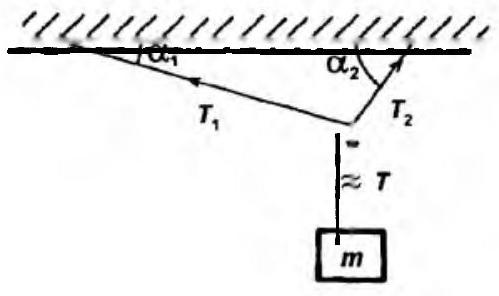
\includegraphics[width=0.4\linewidth]{images/2025_07_01_5b3ff9fa0d508c8e9f17g-017(1)} Fig. 1.5\\

1.68. Pe un plan înclinat cu unghiul $\alpha$ se aşează un corp de masă $m_{1}$ legat de un al doilea corp de masă $m_{2} \left(m_{2}>m_{1}\right)$ printr-un fir trecut peste un scripete ca în Fig. 1.6. $T$ este forţa de tensiune din firul inextensibil, $\mu$ este coeficientul de frecare dintre corpul cu masa $m_{1}$ şi plan, iar mişcarea fiecărui corp se analizează separat, sensul pozitiv de mişcare fiind indicat de săgețile din figură ($x_{1}, x_{2}$ sunt coordonatele şi $a_{1}, a_{2}$ sunt accelerațiile celor două corpuri). Care din următoarele seturi de relații sunt corecte?\\ A) $\mu m_{1} g \cos \alpha+m_{1} g \sin \alpha-T=m_{1} a_{1}, m_{2} g-T=m_{2} a_{2}, x_{1}+x_{2}=\text{ constant }, a_{1}+a_{2}=0$; B) $\mu m_{1} g \cos \alpha-m_{1} g \sin \alpha-T=m_{1} a_{1}, m_{2} g-T=m_{2} a_{2}, x_{1}+x_{2}=\text{ constant }, a_{1}+a_{2}=0$; C) $\mu m_{1} g \cos \alpha+m_{1} g \sin \alpha-T=m_{1} a_{1}, m_{2} g+T=m_{2} a_{2}, x_{1}+x_{2}=\text{ constant }, a_{1}+a_{2}=0$; D) $\mu m_{1} g \cos \alpha-m_{1} g \sin \alpha-T=m_{1} a_{1}, m_{2} g+T=m_{2} a_{2}, x_{1}+x_{2}=\text{ constant }, a_{1}+a_{2}=0$; E) $\mu m_{1} g \cos \alpha+m_{1} g \sin \alpha+T=m_{1} a_{1}, m_{2} g-T=m_{2} a_{2}, x_{1}+x_{2}=\text{ constant }, a_{1}+a_{2}=0$; F) $\mu m_{1} g \cos \alpha+m_{1} g \sin \alpha-T=m_{1} a_{1}, m_{2} g-T=m_{2} a_{2}, x_{1}+x_{2}=\text{ variabil }, a_{1}+a_{2}=\text{ constant }$.\\ (Vasile Popescu)\\ 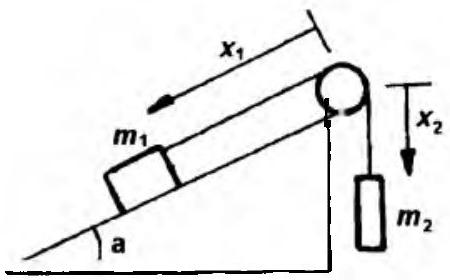
\includegraphics[width=0.4\linewidth]{images/2025_07_01_5b3ff9fa0d508c8e9f17g-017} Fig. 1.6\\

1.69. Două corpuri cu masele $m_{1}=1 \mathrm{~kg}$ şi $m_{2}=2 \mathrm{~kg}$ sunt legate printr-un fir care trece peste un scripete fixat în vârful comun a două plane înclinate ca în Fig. 1.7. Care este valoarea accelerației fiecărui corp? Se consideră $g=9,8 \mathrm{~m} / \mathrm{s}^{2}$.\\ A) $a_{1}=2,97 \mathrm{~m} / \mathrm{s}^{2}, a_{2}=2,97 \mathrm{~m} / \mathrm{s}^{2}$; B) $a_{1}=4,52 \mathrm{~m} / \mathrm{s}^{2}, a_{2}=2,97 \mathrm{~m} / \mathrm{s}^{2}$; C) $a_{1}=6,28 \mathrm{~m} / \mathrm{s}^{2}, a_{2}=6,28 \mathrm{~m} / \mathrm{s}^{2}$; D) $a_{1}=1,12 \mathrm{~m} / \mathrm{s}^{2}, a_{2}=4,52 \mathrm{~m} / \mathrm{s}^{2}$; E) $a_{1}=19,23 \mathrm{~m} / \mathrm{s}^{2}, a_{2}=2,97 \mathrm{~m} / \mathrm{s}^{2}$; F) $a_{1}=10 \mathrm{~m} / \mathrm{s}^{2}, a_{2}=10 \mathrm{~m} / \mathrm{s}^{2}$.\\ (Vasile Popescu)\\ 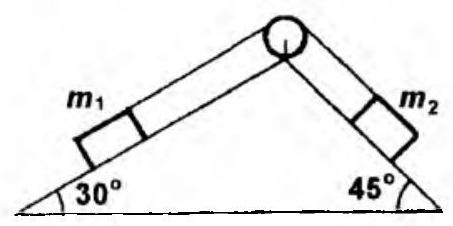
\includegraphics[width=0.4\linewidth]{images/2025_07_01_5b3ff9fa0d508c8e9f17g-018} Fig. 1.7\\

1.70. Un corp este aruncat de jos în sus pe verticală cu viteza inițială $v_{0}$. Al doilea corp cade liber după $\Delta t$ secunde de la înălțimea $h$. Viteza relativă cu care trec cele două corpuri unul pe lângă altul este:\\ A) $v_{0}-g \Delta t$; B) $v_{0}+g \Delta t$; C) $v_{0}-2 g \Delta t$; D) $h \Delta t+v_{0}-g \Delta t$; E) $v_{0}-g \Delta t+h / \Delta t$; F) $v_{0}-g \Delta t-h / \Delta t$.\\ (Vasile Popescu)\\

1.71. Care este condiţia ca un corp aruncat în sus de-a lungul unui plan înclinat să se întoarcă la baza planului?\\ A) $\operatorname{tg} \alpha=\mu$; B) $\sin \alpha=\mu$; C) $\operatorname{tg} \alpha=1 / \mu$; D) $\operatorname{tg} \alpha>\mu$; E) $\operatorname{tg} \alpha<\mu$; F) $\operatorname{ctg} \alpha>\mu$.\\ (Vasile Popescu)\\

1.72. Un biciclist parcurge distanța $d=314 \mathrm{~m}$ pe o traiectorie sub forma unui sfert de cerc. Să se determine raza cercului.\\ A) $100 \mathrm{~m}$; B) $314 \mathrm{~m}$; C) $628 \mathrm{~m}$; D) $200 \mathrm{~m}$; E) $50 \mathrm{~m}$; F) $150 \mathrm{~m}$.\\ (Vasile Popescu)\\

1.73. Un corp cu masa $m=1 \mathrm{~kg}$ este ridicat pe verticală cu accelerația $a=0,19 \mathrm{~m} / \mathrm{s}^{2}$ până la înălțimea $h=10 \mathrm{~m}$. Să se determine lucrul mecanic efectuat ($g=9,81 \mathrm{~m} / \mathrm{s}^{2})$.\\ A) $10 \mathrm{~J}$; B) $150 \mathrm{~J}$; C) $200 \mathrm{~J}$; D) $100 \mathrm{~J}$; E) $981 \mathrm{~J}$; F) $9,81 \mathrm{~J}$.\\ (Vasile Popescu)\\

1.74. Pentru a se mişca uniform, un corp în cădere liberă întâmpină din partea aerului o forță de rezistență de $98,1 \mathrm{~N}$. Să se determine masa corpului ($g=9,81 \mathrm{~m} / \mathrm{s}^{2}$).\\ A) $2 \mathrm{~kg}$; B) $5 \mathrm{~kg}$; C) $10 \mathrm{~kg}$; D) $9,81 \mathrm{~kg}$; E) $98,1 \mathrm{~kg}$; F) $0,981 \mathrm{~kg}$.\\ (Vasile Popescu)\\

1.75. O persoană merge prima jumătate din drumul său total cu viteza $v_{1}=6 \mathrm{~km} / \mathrm{h}$, iar cealaltă jumătate cu viteza $v_{2}=4 \mathrm{~km} / \mathrm{h}$. Care este viteza medie a persoanei?\\ A) $48 \mathrm{~km} / \mathrm{h}$; B) $9,6 \mathrm{~km} / \mathrm{h}$; C) $5 \mathrm{~km} / \mathrm{h}$; D) $4,8 \mathrm{~km} / \mathrm{h}$; E) $8,4 \mathrm{~km} / \mathrm{h}$; F) $10 \mathrm{~km} / \mathrm{h}$.\\ (Vasile Popescu)\\

1.76. Două corpuri paralelipipedice de mase $m_{1}=2 \mathrm{~kg}$ şi $m_{2}=1 \mathrm{~kg}$ sunt suprapuse pe o masă orizontală fară frecări. Corpul cu masa $m_{1}$ în contact cu masa este împins cu o forţă orizontală $F=6 \mathrm{~N}$. Să se determine accelerația sistemului.\\ A) $1 \mathrm{~m} / \mathrm{s}^{2}$; B) $2 \mathrm{~m} / \mathrm{s}^{2}$; C) $3 \mathrm{~m} / \mathrm{s}^{2}$; D) $0,5 \mathrm{~m} / \mathrm{s}^{2}$; E) $4 \mathrm{~m} / \mathrm{s}^{2}$; F) $1,5 \mathrm{~m} / \mathrm{s}^{2}$.\\ (Vasile Popescu)\\

1.77.* Un corp cu masa $m_{1}=10 \mathrm{~kg}$ se află în repaus. Un alt corp cu masa $m_{2}=2 \mathrm{~kg}$ loveşte primul corp cu viteza $v_{0}=30 \mathrm{~m} / \mathrm{s}$. Să se determine viteza finală a celor două corpuri dacă ciocnirea lor este plastică.\\ A) $5 \mathrm{~m} / \mathrm{s}$; B) $2 \mathrm{~m} / \mathrm{s}$; C) $10 \mathrm{~m} / \mathrm{s}$; D) $1 \mathrm{~m} / \mathrm{s}$; E) $3 \mathrm{~m} / \mathrm{s}$; F) $2,5 \mathrm{~m} / \mathrm{s}$.\\ (Vasile Popescu)\\

1.78. Un corp cu energia cinetică inițială $E=24 \mathrm{~J}$ urcă pe un plan înclinat cu unghiul $\alpha=45^{\circ}$ față de orizontală. Coeficientul de frecare între corp şi plan este $\mu=0,2$. Lucrul mecanic al forței de frecare până la oprirea corpului pe plan este:\\ A) $2 \mathrm{~J}$; B) $\frac{\sqrt{2}}{2} \mathrm{~J}$; C) $3 \mathrm{~J}$; D) $4 \mathrm{~J}$; E) $12,2 \mathrm{~J}$; F) $3,6 \mathrm{~J}$.\\ (Mircea Stan)\\

1.79. Un corp cu $m=200 \mathrm{~g}$ cade în $t=3 \mathrm{~s}$ de la înălțimea $h=1,8 \mathrm{~m}$. Forța de rezistență ce acționează asupra corpului este ($g=9,8 \mathrm{~m} / \mathrm{s}^{2}$):\\ A) $0,88 \mathrm{~N}$; B) $1,08 \mathrm{~N}$; C) $1,88 \mathrm{~N}$; D) $2,4 \mathrm{~N}$; E) $2,82 \mathrm{~N}$; F) $4,4 \mathrm{~N}$.\\ (Mircea Stan)\\

1.80. O minge este izbită pe verticală de la înălțimea $h=1,8 \mathrm{~m}$ de pământ. În urma ciocnirii, considerate perfect elastice, mingea se înalță la $h^{\prime}=2 \mathrm{~m}$. Viteza inițială a mingii este ($g=10 \mathrm{~m} / \mathrm{s}^{2}$):\\ A) $20 \mathrm{~m} / \mathrm{s}$; B) $10 \mathrm{~m} / \mathrm{s}$; C) $9,8 \mathrm{~m} / \mathrm{s}$; D) $4 \mathrm{~m} / \mathrm{s}$; E) $3,6 \mathrm{~m} / \mathrm{s}$; F) $2 \mathrm{~m} / \mathrm{s}$.\\ (Mircea Stan)\\

1.81. Un om cântărind $70 \mathrm{~kg}$ susține o greutate de $16 \mathrm{~kg}$ în ajutorul unui fir trecut peste un scripete fix. Care este forța de apăsare normală a omului asupra pământului, dacă firul e înclinat față de verticală cu $60^{\circ}$? ($g=9,8 \mathrm{~m} / \mathrm{s}^{2})$\\ A) $509,3 \mathrm{~N}$; B) $607,6 \mathrm{~N}$; C) $402,6 \mathrm{~N}$; D) $120 \mathrm{~N}$; E) $702,6 \mathrm{~N}$; F) $263 \mathrm{~N}$.\\ (Mircea Stan)\\

1.82. Ce putere are un alpinist de $75 \mathrm{~kg}$ care se ridică în trei minute la $18 \mathrm{~m}$ înălțime? ($g=10 \mathrm{~m} / \mathrm{s}^{2}$)\\ A) $275 \mathrm{~W}$; B) $375 \mathrm{~W}$; C) $100 \mathrm{~W}$; D) $125 \mathrm{~W}$; E) $75 \mathrm{~W}$; F) $30 \mathrm{~W}$.\\ (Mircea Stan)\\

1.83. O piatră aruncată vertical în sus revine la punctul de plecare după $4 \mathrm{~s}$. Neglijând frecările, înălțimea maximă atinsă de piatră este: ($g=10 \mathrm{~m} / \mathrm{s}^{2}$)\\ A) $20 \mathrm{~m}$; B) $16 \mathrm{~m}$; C) $10 \mathrm{~m}$; D) $8 \mathrm{~m}$; E) $4 \mathrm{~m}$; F) $2 \mathrm{~m}$.\\ (Mircea Stan)\\

1.84. Un elev care merge cu tramvaiul ține în mână un fir cu plumb. Când tramvaiul frânează brusc, firul se îndepărtează de la verticală cu unghiul $\alpha=30^{\circ}$. Accelerația de frânare a tramvaiului este: ($g=9,8 \mathrm{~m} / \mathrm{s}^{2}$)\\ A) $2,65 \mathrm{~m} / \mathrm{s}^{2}$; B) $3,42 \mathrm{~m} / \mathrm{s}^{2}$; C) $4,66 \mathrm{~m} / \mathrm{s}^{2}$; D) $5,66 \mathrm{~m} / \mathrm{s}^{2}$; E) $6,23 \mathrm{~m} / \mathrm{s}^{2}$; F) $6,82 \mathrm{~m} / \mathrm{s}^{2}$.\\ (Mircea Stan)\\

1.85.* Un corp $A$ cu masa $m_{A}=0,8 \mathrm{~kg}$ ciocneşte plastic un corp $B$ cu masa $m_{B}=1,2 \mathrm{~kg}$ aflat în repaus. În urma ciocnirii, cele două corpuri se deplasează împreună pe un plan orizontal şi parcurg până la oprire $l=4 \mathrm{~cm}$. Coeficientul de frecare dintre corpuri şi plan fiind $\mu=0,2$ iar $g=10 \mathrm{~m} / \mathrm{s}^{2}$, să se determine viteza initịală a corpului $A$.\\ A) $1 \mathrm{~m} / \mathrm{s}$; B) $1,5 \mathrm{~m} / \mathrm{s}$; C) $2 \mathrm{~m} / \mathrm{s}$; D) $2,5 \mathrm{~m} / \mathrm{s}$; E) $3 \mathrm{~m} / \mathrm{s}$; F) $3,5 \mathrm{~m} / \mathrm{s}$.\\ (Mircea Stan)\\

1.86. Un mobil este aruncat pe verticală, în sus în câmpul gravitațional terestru ($g=9,81 \mathrm{~m} / \mathrm{s}^{2}$) cu viteza $v=20 \mathrm{~m} / \mathrm{s}$. Simultan, dintr-un turn vertical de înălțime $h=40 \mathrm{~m}$ aflat pe aceeaşi verticală cu a primului corp, este aruncat oblic, cu aceeaşi viteză, sub unghiul $\alpha=30^{\circ}$ față de orizontală, un al doilea mobil. Atunci momentul de timp la care distanța dintre mobile este minimă şi această distanță vor fi:\\ A) $t=2 \mathrm{~s}, d=20 \mathrm{~m}$; B) $t=2 \mathrm{~s}, d=20 \sqrt{3} \mathrm{~m}$; C) $t=1 \mathrm{~s}, d=20 \mathrm{~m}$; D) $t=3 \mathrm{~s}, d=40 \mathrm{~m}$; E) $t=1 \mathrm{~s}, d=20 \sqrt{3} \mathrm{~m}$; F) $t=2,5 \mathrm{~s}, d=22 \mathrm{~m}$.\\ (Constantin Roşu)\\

1.87. Un plan înclinat de unghi $\alpha=60^{\circ}$ şi masa $m_{1}=3 \mathrm{~kg}$ se poate deplasa fără frecare pe o suprafață orizontală. El este pus în mişcare sub acțiunea unei forțe orizontale $F=6 \mathrm{~N}$ dirijate în sensul de mişcare naturală a corpurilor pe plan. Pe plan se află un corp de masă $m_{2}=0,2 \mathrm{~kg}$ care se poate deplasa cu frecare pe planul înclinat ($\mu=0,3 ; g=9,8 \mathrm{~m} / \mathrm{s}^{2}$). Atunci corpul $m_{2}$ va avea față de planul înclinat următoarea dinamică:\\ A) urcă uniform pe plan; B) urcă accelerat cu $a=2 \mathrm{~m} / \mathrm{s}^{2}$; C) coboară accelerat cu $a=5,74 \mathrm{~m} / \mathrm{s}^{2}$; D) coboară uniform; E) nu se poate da nici un răspuns cu datele oferite; F) coboară cu accelerația $a=3 \mathrm{~m} / \mathrm{s}^{2}$.\\ (Constantin Roşu)\\

1.88. Un pendul matematic este alcătuit dintr-un fir elastic cu lungimea nedeformată $L=2 \mathrm{~m}$ şi constanta elastică $k=10 \mathrm{~N} / \mathrm{m}$. De pendul este agățat un corp cu masa $m=3 \mathrm{~kg}$ care oscilează cu amplitudinea unghiulară $\alpha=45^{\circ}$. Să se calculeze unghiul $\beta$ făcut de fir cu verticala pentru care viteza pendulului este $1 / 2$ din viteza sa maximă.\\ A) $\cos \beta=0,2$; B) $\cos \beta=0,8$; C) $\sin \beta=0,5$; D) $\cos \beta=0,707$; E) $\sin \beta=0,86$; F) $\cos \beta=-0,5$.\\ (Constantin Roşu)\\

1.89.* Un corp de masă $m_{1}$ şi viteză $v$ ciocneşte perfect elastic un corp de masă $m_{2}$ aflat în repaus. După cionire, vitezele corpurilor $m_{1}$ şi $m_{2}$ fac unghiurile $\alpha$ respectiv $\beta$ cu direcția inițialǎ a particulei 1. Raportul energiilor cinetice ale celor 2 particule după ciocnire este:\\ A) $\frac{E_{c 1}}{E_{c 2}}=\frac{m_{1} \sin ^{2}(\alpha+\beta)}{m_{2} \sin ^{2} \alpha}$; B) $\frac{E_{c 1}}{E_{c 2}}=\frac{m_{2} \sin (\alpha+\beta)}{m_{1} \cos \alpha}$; C) $\frac{E_{c 1}}{E_{c 2}}=\left(\frac{m_{1}}{m_{2}}\right)^{2} \frac{\cos \beta}{\cos ^{2} \alpha}$; D) $\frac{E_{c 1}}{E_{c 2}}=\frac{m_{2} \sin ^{2}(\alpha+\beta)}{\sin ^{2}(\alpha-\beta)}$; E) $\frac{E_{c 1}}{E_{c 2}}=\frac{m_{2} \sin ^{2} \beta}{m_{1} \sin ^{2} \alpha}$; F) $\frac{E_{c 1}}{E_{c 2}}=\left(\frac{2 m_{1}}{m_{2}}\right)^{2} \frac{\cos ^{2} \beta}{\cos ^{2} \alpha}$.\\ (Constantin Roşu)\\

1.90. Un automobil urcă uniform pe un plan înclinat de unghi mic ($\sin \alpha=\alpha, \cos \alpha=1$) cu viteza $v_{1}$. Cu aceeaşi putere a motorului, el va coborî uniform pe planul înclinat cu viteza $v_{2}$. Care este viteza de deplasare pe un plan orizontal, cu putere dublă față de cea folosită pe planul înclinat?\\ A) $v=\frac{v_{1} \cdot v_{2}}{2 v_{1}+v_{2}}$; B) $v=2 \sqrt{v_{1} \cdot v_{2}}$; C) $v=\frac{4 v_{1} \cdot v_{2}}{v_{1}+v_{2}}$; D) $v=\frac{v_{1} \cdot v_{2}}{v_{1}-v_{2}}$; E) $v=\frac{2 v_{1} \cdot v_{2}}{v_{1}+v_{2}}$; F) $v=\frac{v_{1} \cdot v_{2}}{v_{1}-2 v_{2}}$.\\ (Constantin Roşu)\\

1.91. Forța care acționează asupra unui punct material de masă $m$ dintr-un pendul matematic care face unghiul $\alpha$ cu verticala pentru a-l readuce în poziția de echilibru, este:\\ A) $F_{r}=m g \cos \alpha$; B) $F_{r}=m g \sin \alpha$; C) $F_{r}=m g / \cos \alpha$; D) $F_{r}=m g$; E) $F_{r}=m g \operatorname{tg} \alpha$; F) $F_{r}=m g \operatorname{ctg} \alpha$.\\ (Constantin Roşu)\\

1.92. Unui corp aflat pe un plan orizontal cu frecare, $\mu=0,1$, i se imprimă o viteză inițială $v_{0}=8 \mathrm{~m} / \mathrm{s}$. Cât este spațiul parcurs de corp până la oprire? Se dă $g=9,8 \mathrm{~m} / \mathrm{s}^{2}$.\\ A) $23 \mathrm{~m}$; B) $2,3 \mathrm{~m}$; C) $7,3 \mathrm{~m}$; D) $32,65 \mathrm{~m}$; E) $152,3 \mathrm{~cm}$; F) $10 \mathrm{~m}$.\\ (Răzvan Mitroi)\\

1.93. Mişcarea unui corp este descrisă de ecuația $s=a+b t^{2}$ unde $a=20 \mathrm{~cm}$, iar $b=4 \mathrm{~cm} / \mathrm{s}^{2}$. Să se afle spațiul parcurs şi viteza corpului dupã timpul $t=2 \mathrm{~s}$.\\ A) $s=0,36 \mathrm{~m}, v=0,16 \mathrm{~m} / \mathrm{s}$; B) $s=6 \mathrm{~m}, v=7,6 \mathrm{~m} / \mathrm{s}$; C) $s=3 \mathrm{~m}, v=1,6 \mathrm{~m} / \mathrm{s}$; D) $s=0,36 \mathrm{~cm}, v=0,16 \mathrm{~cm} / \mathrm{s}$; E) $s=5 \mathrm{~m}, v=4,16 \mathrm{~m} / \mathrm{s}$; F) $s=0,4 \mathrm{~m}, v=0,15 \mathrm{~m} / \mathrm{s}$.\\ (Răzvan Mitroi)\\

1.94. Un corp cade liber de la înălțimea $h=1960 \mathrm{~m}$. Să se determine timpul în care sunt parcurşi ultimii $60 \mathrm{~m}$. Se dă $g=9,8 \mathrm{~m} / \mathrm{s}^{2}$.\\ A) $0,31 \mathrm{~s}$; B) $13 \mathrm{~s}$; C) $31 \mathrm{~s}$; D) $15 \mathrm{~s}$; E) $5,3 \mathrm{~s}$; F) $12 \mathrm{~s}$.\\ (Răzvan Mitroi)\\

1.95. 0 minge este aruncată orizontal cu viteza $v_{0}=5 \mathrm{~m} / \mathrm{s}$. Să se determine viteza şi poziția sa după timpul $t=0,5 \mathrm{~s}$. Se dă $g=10 \mathrm{~m} / \mathrm{s}^{2}$.\\ A) $v=5 \sqrt{2} \mathrm{~m} / \mathrm{s}, x=5 \mathrm{~m}, y=1,25 \mathrm{~m}$; B) $v=5 \sqrt{2} \mathrm{~m} / \mathrm{s}, x=5 \mathrm{~m}, y=1,25 \mathrm{~m}$; C) $v=5 \mathrm{~m} / \mathrm{s}, x=5 \mathrm{~m}, y=1,25 \mathrm{~m}$; D) $v=5 \sqrt{2} \mathrm{~m} / \mathrm{s}, x=2,5 \mathrm{~m}, y=1,25 \mathrm{~m}$; E) $v=5 \sqrt{2} \mathrm{~m} / \mathrm{s}, x=0,5 \mathrm{~m}, y=12,5 \mathrm{~m}$; F) $v=3 \sqrt{2} \mathrm{~m} / \mathrm{s}, x=2,5 \mathrm{~m}, y=1,20 \mathrm{~m}$.\\ (Răzvan Mitroi)\\

1.96. Un biciclist s-a deplasat din punctul $A$ în punctul $B$ cu viteza $v_{1}=12 \mathrm{~km} / \mathrm{h}$, iar la întoarcerea din $B$ în $A$ cu viteza $v_{2}=8 \mathrm{~km} / \mathrm{h}$. Viteza medie a biciclistului este:\\ A) $10 \mathrm{~km} / \mathrm{h}$; B) $9,2 \mathrm{~km} / \mathrm{h}$; C) $20 \mathrm{~km} / \mathrm{h}$; D) $10,5 \mathrm{~km} / \mathrm{h}$; E) $9,6 \mathrm{~km} / \mathrm{h}$; F) $10,6 \mathrm{~km} / \mathrm{h}$.\\ (Ion Belciu)\\

1.97. Două corpuri de mase $m_{1}=0,2 \mathrm{~kg}$ şi $m_{2}=0,6 \mathrm{~kg}$ sunt legate printr-un fir şi trase în sus cu o forţă $F=8 \mathrm{~N}$. Considerând accelerația gravitațională $g=9,8 \mathrm{~m} / \mathrm{s}^{2}$, tensiunea mecanică din firul de legătură este egală cu:\\ A) $8 \mathrm{~N}$; B) $7,8 \mathrm{~N}$; C) $6,25 \mathrm{~N}$; D) $6 \mathrm{~N}$; E) $10 \mathrm{~N}$; F) $6,7 \mathrm{~N}$.\\ (Ion Belciu)\\

1.98. Un corp este aruncat pe verticală în sus cu viteza $v_{01}=20 \mathrm{~m} / \mathrm{s}$. După ce ajunge la înălțimea maximă, este aruncat în același mod un corp cu viteza inițială $v_{02}=10 \mathrm{~m} / \mathrm{s}$. Cunoscând accelerația gravitațională $g=10 \mathrm{~m} / \mathrm{s}^{2}$, timpul (în raport cu aruncarea celui de-al doilea corp) în care corpurile se întâlnesc este:\\ A) $9,2 \mathrm{~s}$; B) $5 \mathrm{~s}$; C) $10 \mathrm{~s}$; D) $2 \mathrm{~s}$; E) $2,5 \mathrm{~s}$; F) $4 \mathrm{~s}$.\\ (Ion Belciu)\\

1.99. Un corp de masă $m$, se mişcă uniform pe un plan orizontal sub acțiunea unei forțe $F$ aplicată ca în Fig. 1.8. Cunoscând accelerația gravitațională $g$, coeficientul de frecare dintre corp şi plan va fi:\\ A) $F+m g$; B) $\frac{m g \sin \alpha}{F}$; C) $\frac{m g+F \cos \alpha}{F \sin \alpha}$; D) $\frac{F \cos \alpha}{m g+F}$; E) $\frac{F \cos \alpha}{m g+F \sin \alpha}$; F) $F \operatorname{tg} \alpha$.\\ (Ion Belciu)\\ 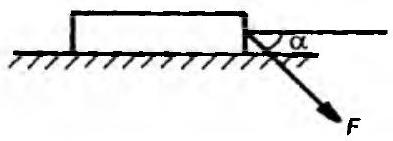
\includegraphics[width=0.4\linewidth]{images/2025_07_01_5b3ff9fa0d508c8e9f17g-024} Fig. 1.8.\\

1.100. De un tren cu masa $M=110 \mathrm{t}$, care merge rectiliniu şi uniform, se desprinde la un moment dat ultimul vagon de masă $m=10 \mathrm{t}$. Vagonul parcurge o distanță $d=10 \mathrm{~km}$ până se opreşte. Considerând că forțele de frecare sunt proporționale cu greutatea şi că forța de tracțiune a locomotivei trenului a rămas constantă, distanța dintre vagonul oprit şi tren în momentul în care se opreşte vagonul este:\\ A) $32 \mathrm{~km}$; B) $25 \mathrm{~km}$; C) $12 \mathrm{~km}$; D) $24 \mathrm{~km}$; E) $11 \mathrm{~km}$; F) $12,5 \mathrm{~km}$.\\ (Ion Belciu)\\

1.101.* Un aviator de masă $m=70 \mathrm{~kg}$ execută un cerc de rază $R=800 \mathrm{~m}$ în plan vertical, cu viteza $v=700 \mathrm{~km} / \mathrm{h}$. Considerând accelerația gravitațională $g=10 \mathrm{~m} / \mathrm{s}^{2}$, forța maximă cu care aviatorul apasă asupra scaunului este:\\ A) $300 \mathrm{~N}$; B) $7500 \mathrm{~N}$; C) $4200 \mathrm{~N}$; D) $3000 \mathrm{~N}$; E) $5200 \mathrm{~N}$; F) $700 \mathrm{~N}$.\\ (Ion Belciu)\\

1.102.* O săgeată de masă $m=0,2 \mathrm{~kg}$ şi cu viteza $v_{1}=15 \mathrm{~m} / \mathrm{s}$ pătrunde într-o bilă de plastilină de masă $M=0,3 \mathrm{~kg}$ şi care se află în repaus, formând un singur corp. Energia cinetică a corpului format este:\\ A) $20 \mathrm{~J}$; B) $16,2 \mathrm{~J}$; C) $8 \mathrm{~J}$; D) $9 \mathrm{~J}$; E) $785 \mathrm{~J}$; F) $5 \mathrm{~J}$.\\ (Ion Belciu)\\

1.103. Un corp este aruncat cu viteza inițială $v_{0}$ de-a lungul unui plan înclinat cu unghiul $\alpha=30^{\circ}$ față de un plan orizontal, parcurgând o distanță $l=10 \mathrm{~m}$, fără frecare. Considerând accelerația gravitațională $g=10 \mathrm{~m} / \mathrm{s}^{2}$, valoarea vitezei $v_{0}$ este egală cu:\\ A) $9,8 \mathrm{~m} / \mathrm{s}$; B) $7 \mathrm{~m} / \mathrm{s}$; C) $12 \mathrm{~m} / \mathrm{s}$; D) $10 \mathrm{~m} / \mathrm{s}$; E) $8 \mathrm{~m} / \mathrm{s}$; F) $11 \mathrm{~m} / \mathrm{s}$.\\ (Ion Belciu)\\

1.104.* Un corp cu masa $m_{1}=100 \mathrm{~kg}$ care se mişcă cu viteza $v_{1}=15 \mathrm{~m} / \mathrm{s}$ spre un alt corp cu masa de $1300 \mathrm{~kg}$, care inițial stă pe loc. Care este viteza comună a celor două corpuri, după ciocnirea lor plastică? Care este pierderea de energie cinetică în procesul de ciocnire?\\ A) $u=6,25 \mathrm{~m} / \mathrm{s}, \Delta E_{c}=67500 \mathrm{~J}$; B) $u=6 \mathrm{~m} / \mathrm{s}, \Delta E_{c}=65000 \mathrm{~J}$; C) $u=23,47 \mathrm{~km} / \mathrm{h}, \Delta E_{c}=65 \mathrm{~kJ}$; D) $u=6,52 \mathrm{~m} / \mathrm{s}, \Delta E_{c}=63587 \mathrm{~J}$; E) $E_{1} u=5 \mathrm{~m} / \mathrm{s}, \Delta E_{c}=64580 \mathrm{~J}$; F) $u=5,62 \mathrm{~m} / \mathrm{s}, \Delta E_{c}=65387 \mathrm{~J}$.\\ (Elena Slavnicu)\\

1.105. Alegeți relația corectă reprezentând legea lui Hooke a deformărilor elastice (notații uzuale):\\ A) $F=\frac{E S_{0} l}{\Delta l_{0}}$; B) $\Delta l=\frac{F l_{0}}{E}$; C) $\Delta l=E \sigma l_{0}$; D) $\sigma=\frac{\varepsilon}{E}$; E) $F=\frac{E \Delta l}{l_{0} S_{0}}$; F) $E=\frac{F}{\varepsilon S_{0}}$.\\ (Elena Slavnicu)\\

1.106. Graficul din Fig 1.9 reprezintă dependența de timp a vitezei pentru trei mobile numerotate 1, 2, 3. Alegeți afirmația corectă referitoare la accelerațiile lor:\\ A) $a_{1}=a_{2}=0$, iar $a_{3}$ este pozitivă; B) $a_{2}=0, a_{1}$ şi $a_{3}$ sunt pozitive, $a_{1}>a_{3}$; C) $a_{1}$ şi $a_{2}$ sunt pozitive, iar $a_{3}$ este negativă; D) $a_{2}=0, a_{1}$ şi $a_{3}$ sunt negative, $a_{1}<a_{3}$; E) $a_{2}=0, a_{1}$ şi $a_{3}$ sunt pozitive, $a_{1}<a_{3}$; F) $a_{2}=0, a_{1}$ este pozitivă, iar $a_{3}$ este negativă.\\ (Elena Slavnicu)\\ 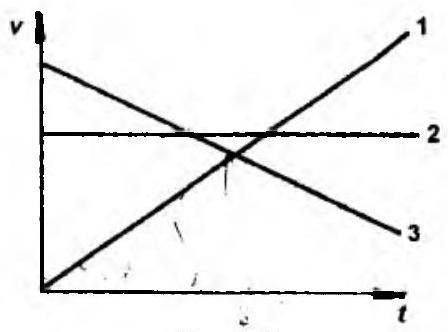
\includegraphics[width=0.4\linewidth]{images/2025_07_01_5b3ff9fa0d508c8e9f17g-025} Fig 1.9\\

1.107. Două corpuri având masele $m_{1}=2 \mathrm{~kg}$ şi $m_{2}=3 \mathrm{~kg}$ sunt legate printr-un fir inextensibil trecut peste un scripete ideal, fixat la marginea unei mese orizontale. Corpul $m_{2}$ atârnă pe verticală, în aer. Între corpul $m_{1}$ şi planul mesei există frecare. Accelerația sistemului este $a=5 \mathrm{~m} / \mathrm{s}^{2}$. Considerând $g=10 \mathrm{~m} / \mathrm{s}^{2}$ şi $\sqrt{2} \cong 1,4$ să se calculeze coeficientul de frecare şi forța care acționează la axul scripetelui.\\ A) $0,15, 24 \mathrm{~N}$; B) $0,25, 21 \mathrm{~N}$; C) $0,85, 15,5 \mathrm{~N}$; D) $0,35, 18 \mathrm{~N}$; E) $0,55, 17 \mathrm{~N}$; F) Nicio variantă nu este corectă.\\ (Nicoleta Eşeanu)\\

1.108. Forța de rupere a unui cablu este cu $40 \%$ mai mare decât tensiunea la care este supus cablul în ridicarea unui corp de masă $m=5 \mathrm{~kg}$ cu accelerația $a=3 \mathrm{~m} / \mathrm{s}^{2}$. Considerând $g=10 \mathrm{~m} / \mathrm{s}^{2}$, să se calculeze masa maximă care poate fi ridicată uniform cu acest cablu.\\ A) $3,45 \mathrm{~kg}$; B) $7,2 \mathrm{~kg}$; C) $7,85 \mathrm{~kg}$; D) $9,1 \mathrm{~kg}$; E) $10,8 \mathrm{~kg}$; F) $11,7 \mathrm{~kg}$.\\ (Nicoleta Eşeanu)\\

1.109.* Un satelit descrie o orbită circulară în jurul Pământului, la înălțimea $h=15 R$, unde $R \cong 6400 \mathrm{~km}$ este raza Pământului, considerat sferic. Se cunoaşte accelerația gravitațională la suprafața Pământului $g=9,8 \mathrm{~m} / \mathrm{s}^{2}$. Viteza satelitului pe orbită şi perioada mişcării sunt:\\ A) $2,8 \mathrm{~km} / \mathrm{s}, 25 \mathrm{~h}$; B) $2,5 \mathrm{~km} / \mathrm{s}, 32,8 \mathrm{~h}$; C) $2,8 \sqrt{2} \mathrm{~km} / \mathrm{s}, 89 \mathrm{~min}$; D) $125,5 \mathrm{~m} / \mathrm{s}, 85 \mathrm{~h}$; E) $1,4 \sqrt{2} \mathrm{~km} / \mathrm{s}, 114 \mathrm{~h}$; F) $1,4 \sqrt{2} \mathrm{~km} / \mathrm{s}, 127,6 \mathrm{~h}$.\\ (Nicoleta Eşeanu)\\

1.110. Pe un plan înclinat de unghi $\alpha=30^{\circ}$ se află un corp cu masa $m_{1}=600 \mathrm{~g}$, legat printr-un fir inextensibil de un alt corp având masa $m_{2}=900 \mathrm{~g}$. Firul este trecut peste un scripete ideal fixat în vârful planului înclinat, corpul $m_{2}$ atârnând pe verticală, în aer. Coeficientul de frecare dintre corpul $m_{1}$ şi plan este $\mu=2 \sqrt(3)$, iar $g=10 \mathrm{~m} / \mathrm{s}^{2}$. În aceste condiții accelerația sistemului şi tensiunea firului sunt:\\ A) $1 \mathrm{~m} / \mathrm{s}^{2}, 8,1 \mathrm{~N}$; B) $2 \mathrm{~m} / \mathrm{s}^{2}, 7,2 \mathrm{~N}$; C) $3 \mathrm{~m} / \mathrm{s}^{2}, 6,3 \mathrm{~N}$; D) $4 \mathrm{m} \mathrm{~s}^{2}, 5,4 \mathrm{~N}$; E) $2 \mathrm{~m} / \mathrm{s}^{2}, 10,8 \mathrm{~N}$; F) $3 \mathrm{~m} / \mathrm{s}^{2}, 11,7 \mathrm{~N}$. \\ (Nicoleta Eşeanu)\\

1.111. Un corp cu masa $m=800 \mathrm{~g}$ este lansat în sus de-a lungul unui plan înclinat cu viteza $v_{0}=4 \mathrm{~m} / \mathrm{s}$. Corpul revine la baza planului înclinat având, în momentul respectiv, viteza $v=0,6 v_{0}$. Lucrul mecanic al forței de frecare dintre corp şi planul înclinat este:\\ A) $-0.58 \mathrm{~J}$; B) $0,85 \mathrm{~J}$; C) $-2,8 \mathrm{~J}$; D) $-4 \mathrm{~J}$; E) $-7,2 \mathrm{~J}$; F) $4,4 \mathrm{~J}$.\\ (Nicoleta Eşeanu)\\

1.112.* Un pendul conic este format dintr-un corp punctiform având masa $m=400 \mathrm{~g}$ suspendat printr-un fir de lungime $l=0,4 \mathrm{~m}$ şi masă neglijabilă. Corpul se află în mişcare de rotație uniformă în plan orizontal cu viteza unghiulară $\omega=5 \mathrm{~rads}$. Accelerația gravitațională este $g=9,8 \mathrm{~m} / \mathrm{s}^{2}$. Să se calculeze unghiul dintre fir şi verticală.\\ A) $160^{\circ}, 0,336 \mathrm{~J} \cdot \mathrm{~s}$; B) $45^{\circ}, 0,6 \mathrm{~J} \cdot \mathrm{~s}$; C) $60^{\circ}, 1,36 \mathrm{~J} \cdot \mathrm{~s}$; D) $30^{\circ}, 0,2 \mathrm{~J} \cdot \mathrm{~s}$; E) $30^{\circ}, 3,58 \mathrm{~J} \cdot \mathrm{~s}$; F) $45^{\circ}, 0,8 \mathrm{~J} \cdot \mathrm{~s}$.\\ (Nicoleta Eşeanu)\\

1.113. Două corpuri de mase $m_{1}=200 \mathrm{~g}$ şi $m_{2}=800 \mathrm{~g}$ sunt lansate unul spre celălalt cu vitezele $v_{1}=6 \mathrm{~m} / \mathrm{s}$ şi respectiv $v_{2}=2,5 \mathrm{~m} / \mathrm{s}$. Ciocnirea lor este unidimensională şi perfect plastică. Viteza sistemului după ciocnire şi căldura dezvoltată în acest proces sunt:\\ A) $2,8 \mathrm{~m} / \mathrm{s}$, în sensul vitezei $v_{1}, Q=3,6 \mathrm{~J}$; B) $3,2 \mathrm{~m} / \mathrm{s}$, in sensul vitezei $v_{1}, Q=9,8 \mathrm{~J}$; C) $0.8 \mathrm{~m} / \mathrm{s}$, în sensul vitezei $v_{2}, Q=5,78 \mathrm{~J}$; D) $0,4 \mathrm{~m} / \mathrm{s}$, în sensul vitezei $v_{2}, Q=2,56 \mathrm{~J}$; E) $5 / 3 \mathrm{~m} / \mathrm{s}$, în sensul vitezei $v_{1}, Q=0,98 \mathrm{~J}$; F) $0,8 \mathrm{~m} / \mathrm{s}$, în sensul vitezei $v_{1}, Q=9,8 \mathrm{~J}$. \\ (Nicoleta Eşeanu)\\

1.114. O moleculă de masă $m=5 \cdot 10^{-26} \mathrm{~kg}$ loveşte perfect elastic un perete vertical, sub un unghi de $60^{\circ}$ faţă de perete. Viteza moleculei înainte de ciocnire este $v=500 \mathrm{~m} / \mathrm{s}$, iar durata ciocnirii este $\Delta t=5 \mathrm{~ms}$. Forța medie cu care peretele acționează asupra moleculei pe durata ciocnirii este:\\ A) $5,6 \cdot 10^{-23} \mathrm{~N}$; B) $3,4 \cdot 10^{-26} \mathrm{~N}$; C) $2,2 \cdot 10^{-22} \mathrm{~N}$; D) $1,86 \cdot 10^{-23} \mathrm{~N}$; E) $8,65 \cdot 10^{-21} \mathrm{~N}$; F) $4,4 \cdot 10^{-22} \mathrm{~N}$.\\ (Nicoleta Eşeanu)\\

1.115.* Un corp punctiform, de masă $m_{1}=200 \mathrm{~g}$, se deplasează cu viteza $v$ pe un plan orizontal şi ciocneşte perfect plastic un alt corp punctiform, de masă $m_{2}=3 m_{1}$. Al doilea corp este legat printr-un resort orizontal, având constanta elastică $k=800 \mathrm{~N} / \mathrm{m}$, de un suport fix. Coeficientul de frecare la alunecare este $\mu=0,225$. Dupã ciocnire sistemul parcurge până la oprire o distanţă de $2 \mathrm{~cm}$. Considerând $g=10 \mathrm{~m} / \mathrm{s}^{2}$, să se calculeze viteza primului corp înainte de ciocnire.\\ A) $2,8 \mathrm{~m} / \mathrm{s}$; B) $1,2 \mathrm{~m} / \mathrm{s}$; C) $0,8 \sqrt{5} \mathrm{~m} / \mathrm{s}$; D) $7 \mathrm{~m} / \mathrm{s}$; E) $2,4 \mathrm{~m} / \mathrm{s}$; F) $3,2 \mathrm{~m} / \mathrm{s}$.\\ (Nicoleta Eşeanu)\\

1.116.* Un disc orizontal de rază $R$ se roteşte în jurul axului său vertical. Pe un cerc de rază $r<R$, cu centrul în centrul discului, sunt practicate opt orificii circulare, egale și echidistante, numerotate de la 1 la 8. De la inălțimea $h=14,7 \mathrm{~m}$, pe verticala orificiului 1, este lăsat să cadă liber un corp punctiform. Cu ce frecvență minimă trebuie să se rotească discul astfel încât corpul să treacă prin orificiul 7? Se consideră $g=9,8 \mathrm{~m} / \mathrm{s}^{2}$.\\ A) $\frac{3}{8} \mathrm{~rot} / \mathrm{min}$; B) $\frac{\pi}{8} \mathrm{~rot} / \mathrm{s}$; C) $\frac{\sqrt{3}}{4} \mathrm{~rot} / \mathrm{s}$; D) $\frac{\pi}{\sqrt{3}} \mathrm{~rot} / \mathrm{min}$; E) $\frac{\sqrt{3}}{8} \mathrm{~rot} / \mathrm{s}$; F) $\frac{\sqrt{3}}{6} \mathrm{~rot} / \mathrm{min}$.\\ (Nicoleta Eşeanu)\\

1.117. Un corp este aruncat în sus în câmp gravitațional cu viteza inițialǎ $v_{0}=40 \mathrm{~m} / \mathrm{s}$. Un alt corp, aflat pe aceeaşi verticală, la înălțimea $H=200 \mathrm{~m}$, este lăsat liber în momentul aruncării primului corp. Considerând $g=10 \mathrm{~m} / \mathrm{s}^{2}$, să se calculeze timpul şi înălțimea la care se produce întâlnirea corpurilor.\\ A) $2,5 \mathrm{~s}, 168,75 \mathrm{~m}$; B) $3 \mathrm{~s}, 155 \mathrm{~m}$; C) $3,6 \mathrm{~s}, 135,2 \mathrm{~m}$; D) $4 \mathrm{~s}, 120 \mathrm{~m}$; E) $5 \mathrm{~s}, 75 \mathrm{~m}$; F) $6 \mathrm{~s}, 20 \mathrm{~m}$.\\ (Nicoleta Eşeanu)\\

1.118. Două corpuri de masa $m$ sunt legate printr-un fir inextensibil care este trecut peste un scripete fix. Pe corpul din stânga se aşează o greutate de masă $m_{0}$. Accelerația sistemului are expresia:\\ A) $\frac{2 m g}{m_{0}+m}$; B) $\frac{m_{0} g}{m+2 m_{0}}$; C) $\frac{m g}{2 m+m_{0}}$; D) $\frac{m_{0} g}{2 m+m_{0}}$; E) $\frac{m g}{2 m_{0}+m}$; F) $\frac{2 m_{0} g}{m_{0}+m}$.\\ (Daniela Buzatu)\\

1.119. O şalupă se deplasează pe un râu din punctul A spre punctul B în timpul $t_{1}$, şi înapoi în timpul $t_{2}$. Cât timp îi este necesar şalupei să parcurgă aceeaşi distanță AB cu motorul oprit?\\ A) $\frac{2 t_{1} t_{2}}{t_{1}+t_{2}}$; B) $\frac{2 t_{1} t_{2}}{2 t_{2}-t_{1}}$; C) $\frac{2 t_{1} t_{2}}{t_{2}-t_{1}}$; D) $\frac{t_{1} t_{2}}{t_{1}+t_{2}}$; E) $\frac{2 t_{1} t_{2}}{2 t_{1}-t_{2}}$; F) $\frac{t_{1} t_{2}}{t_{2}-t_{1}}$.\\ (Daniela Buzatu)\\

1.120. Viteza medie a unui călātor care parcurge primul sfert din timp cu viteza $v_{1}=7 \mathrm{~km} / \mathrm{h}$, iar restul timpului cu viteza $v_{2}=4 \mathrm{~km} / \mathrm{h}$ şi viteza medie a unui alt călător care parcurge primul sfert din drum cu viteza $v_{1}=7 \mathrm{~km} / \mathrm{h}$, iar restul drumului cu viteza $v_{2}=4 \mathrm{~km} / \mathrm{h}$, sunt:\\ A) $4,25 \mathrm{~km} / \mathrm{h}, 8,84 \mathrm{~km} / \mathrm{h}$; B) $4,75 \mathrm{~km} / \mathrm{h}, 4,48 \mathrm{~km} / \mathrm{h}$; C) $5,75 \mathrm{~km} / \mathrm{h}, 4,88 \mathrm{~km} / \mathrm{h}$; D) $5,57 \mathrm{~km} / \mathrm{h}, 8,48 \mathrm{~km} / \mathrm{h}$; E) $7,75 \mathrm{~km} / \mathrm{h}, 4,84 \mathrm{~km} / \mathrm{h}$; F) $7,25 \mathrm{~km} / \mathrm{h}, 8,88 \mathrm{~km} / \mathrm{h}$.\\ (Daniela Buzatu)\\

1.121. O minge de masă $m=0,2 \mathrm{~kg}$ cade de la înălțimea de $1 \mathrm{~m}$ cu accelerația $a=8 \mathrm{~m} / \mathrm{s}^{2}$. Variația impulsului mingii este:\\ A) $0,5657 \mathrm{~kg} \mathrm{~m} / \mathrm{s}$; B) $0,8 \mathrm{~kg} \mathrm{~m} / \mathrm{s}$; C) $0,4 \mathrm{~kg} \mathrm{~m} / \mathrm{s}$; D) $2,8284 \mathrm{~kg} \mathrm{~m} / \mathrm{s}$; E) $0,2828 \mathrm{~kg} \mathrm{~m} / \mathrm{s}$; F) $0,8854 \mathrm{~kg} \mathrm{~m} / \mathrm{s}$.\\ (Daniela Buzatu)\\

1.122. Un automobil se deplasează cu viteza $v=72 \mathrm{~km} / \mathrm{h}$ pe un podeț ce are aspectul unui arc de cerc. În punctul superior al podețului forța sa de apăsare normală se micşorează de două ori ($g=10 \mathrm{~m} / \mathrm{s}^{2}$). Raza podețului este:\\ A) $40 \mathrm{~m}$; B) $14,4 \mathrm{~m}$; C) $80 \mathrm{~m}$; D) $4 \mathrm{~m}$; E) $8 \mathrm{~m}$; F) $72 \mathrm{~m}$.\\ (Daniela Buzatu)\\

1.123. O piatră de masă $m=5 \mathrm{~kg}$ este aruncată vertical în jos de la înălțimea $h=5 \mathrm{~m}$ cu viteza inițială $v_{0}=2 \mathrm{~m} / \mathrm{s}$. Înainte de impactul cu Pământul, viteza pietrei era $v=4 \mathrm{~m} / \mathrm{s}$. Lucrul mecanic al forței de rezistență a aerului este:\\ A) $+220 \mathrm{~J}$; B) $-220 \mathrm{~J}$; C) $-190 \mathrm{~J}$; D) $+190 \mathrm{~J}$; E) $+470 \mathrm{~J}$; F) $-470 \mathrm{~J}$.\\ (Daniela Buzatu)\\

1.124. Pentru a menține constantă viteza unei sănii pe un drum orizontal trebuie să acționăm cu o forță $F_{1}=120 \mathrm{~N}$ sub un unghi $\alpha_{1}=60^{\circ}$ față de orizontală, sau cu o forță $F_{2}=50 \sqrt{3} \mathrm{~N}$ sub un unghi $\alpha_{2}=30^{\circ}$, considerând $g=10 \mathrm{~m} / \mathrm{s}^{2}$. Între sanie şi drum există frecare. Masa saniei are valoarea:\\ A) $60 / 7 \mathrm{~kg}$; B) $20 \sqrt{3} \mathrm{~kg}$; C) $7 / 60 \mathrm{~kg}$; D) $40 \sqrt{3} \mathrm{~kg}$; E) $10 \sqrt{3} \mathrm{~kg}$; F) $60 \sqrt{3} \mathrm{~kg}$.\\ (Daniela Buzatu)\\

1.125. Un proiectil cu masa $m=5 \mathrm{~kg}$ şi cu viteza $v_{0}=300 \mathrm{~m} / \mathrm{s}$ intră într-un strat de zăpadă de lungime $l=10 \mathrm{~km}$. Stratul absoarbe prin frecare o cantitate de căldură $Q=200 \mathrm{~kJ}$. Viteza la ieşirea din strat, accelerația şi timpul în care proiectilul străbate stratul de zăpadă sunt:\\ A) $100 \mathrm{~m} / \mathrm{s}, -4 \mathrm{~m} / \mathrm{s}^{2}, 50 \mathrm{~s}$; B) $200 \mathrm{~m} / \mathrm{s}, -2 \mathrm{~m} / \mathrm{s}^{2}, 25 \mathrm{~s}$; C) $200 \mathrm{~m} / \mathrm{s}, -2 \mathrm{~m} / \mathrm{s}^{2}, 50 \mathrm{~s}$; D) $100 \mathrm{~m} / \mathrm{s}, +4 \mathrm{~m} / \mathrm{s}^{2}, 50 \mathrm{~s}$; E) $200 \mathrm{~m} / \mathrm{s}, +2 \mathrm{~m} / \mathrm{s}^{2}, 25 \mathrm{~s}$; F) $100 \mathrm{~m} / \mathrm{s}, -4 \mathrm{~m} / \mathrm{s}^{2}, 25 \mathrm{~s}$.\\ (Daniela Buzatu)\\

1.126. Un corp aruncat orizontal din vârful unui plan înclinat spre bază cade pe plan la distanţa $l=30 \mathrm{~m}$ de vârf. Cunoscând înclinația planului față de $\mathrm{O} x$, $\alpha=30^{\circ}$ şi $g=10 \mathrm{~m} \cdot \mathrm{~s}^{-2}$, viteza inițială $v_{0}$ cu care este aruncat corpul are valoarea:\\ A) $10 \mathrm{~m} \cdot \mathrm{~s}^{-1}$; B) $12 \mathrm{~m} \cdot \mathrm{~s}^{-1}$; C) $15 \mathrm{~m} \cdot \mathrm{~s}^{-1}$; D) $0,1 \mathrm{~m} \cdot \mathrm{~s}^{-1}$; E) $1,2 \mathrm{~m} \cdot \mathrm{~s}^{-1}$; F) $1,5 \mathrm{~m} \cdot \mathrm{~s}^{-1}$.\\ (Ilie Ivanov)\\

1.127. Două corpuri de masă $M$, respectiv $m (M>m)$ sunt legate între ele printr-un fir de legătură de greutate neglijabilă şi se află pe o suprafață orizontală aşa cum arată Fig. 1.10. Dacă sistemul este acționat de o forță orizontală $F$ ce acționează asupra corpului de masă $m$, sistemul se va mişca accelerat cu accelerația $a_{1}$, tensiunea în firul de legătură fiind $T_{1}$ (caz 1). Dacă însă aceeaşi forță actionează asupra corpului de masă $M$, accelerația sistemului va fi $a_{2}$ şi tensiunea $T_{2}$ (caz 2). În aceste condiții, care este relaţia dintre mărimi?\\ A) $a_{1}=a_{2}, T_{1}>T_{2}$; B) $a_{1}>a_{2}, T_{1}<T_{2}$; C) $a_{1}<a_{2}, T_{1}>T_{2}$; D) $a_{1}<a_{2}, T_{1}<T_{2}$; E) $a_{1}>a_{2}, T_{1}=T_{2}$; F) $a_{1}=a_{2}, T_{1}=T_{2}$.\\ (Ilie Ivanov)\\ 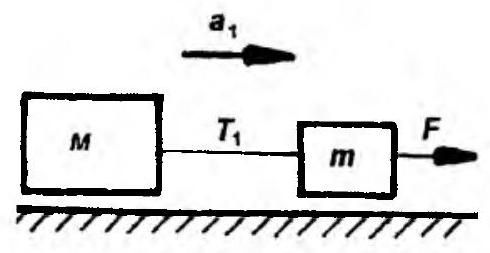
\includegraphics[width=0.4\linewidth]{images/2025_07_01_5b3ff9fa0d508c8e9f17g-031(1)} Caz 1, 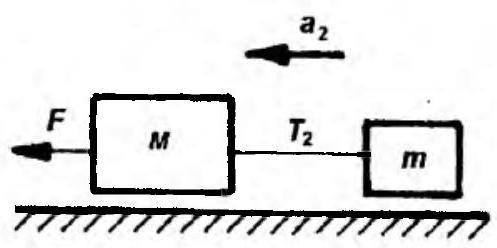
\includegraphics[width=0.4\linewidth]{images/2025_07_01_5b3ff9fa0d508c8e9f17g-031} Caz 2, Fig. 1.10\\

1.128. Două resorturi de constante elastice $k_{1}$, respectiv $k_{2}$, legate în serie susțin un corp de masă $M$. Raportul între energiile potentiale ale resorturilor este:\\ A) $\frac{E_{1}}{E_{2}}=\frac{k_{1}}{k_{2}}$; B) $\frac{E_{1}}{E_{2}}=\frac{k_{2}}{k_{1}}$; C) $\frac{E_{1}}{E_{2}}=\frac{k_{1}^{2}}{k_{2}^{2}}$; D) $\frac{E_{1}}{E_{2}}=\frac{k_{2}^{2}}{k_{1}^{2}}$; E) $\frac{E_{1}}{E_{2}}=\frac{k_{1}+k_{2}}{k_{1}-k_{2}}$; F) $\frac{E_{1}}{E_{2}}=\frac{k_{1}-k_{2}}{k_{1}+k_{2}}$.\\ (Ilie Ivanov)\\

1.129. Un patinator de masă $M=80 \mathrm{~kg}$ ține în mână o bilă de masă $m=8 \mathrm{~kg}$ care se află în repaus pe gheață. La un moment dat aruncă bila înainte cu viteza $v=10 \mathrm{~m} \cdot \mathrm{~s}^{-1}$. Cunoscând $g=10 \mathrm{~m} \cdot \mathrm{~s}^{-2}$ şi coeficientul de frecare cu gheața $\mu=0,001$, spațiul parcurs de patinator în urma acestei operații este:\\ A) $50 \mathrm{~m}$; B) $60 \mathrm{~m}$; C) $70 \mathrm{~m}$; D) $5 \mathrm{~m}$; E) $0,6 \mathrm{~m}$; F) $4,5 \mathrm{~m}$.\\ (Ilie Ivanov)\\

1.130. Viteza unui mobil este dată de relația $v=m+n t^{2}$, unde $m=16 \mathrm{~cm} / \mathrm{s}$, iar $n=0,8 \mathrm{~cm} / \mathrm{s}^{2}$. Să se afle viteza şi accelerația instantanee la momentul $t=5 \mathrm{~s}$.\\ A) $v=1 \mathrm{~m} / \mathrm{s}, a=0,8 \mathrm{~m} / \mathrm{s}^{2}$; B) $v=2 \mathrm{~m} / \mathrm{s}, a=1 \mathrm{~m} / \mathrm{s}^{2}$; C) $v=0,18 \mathrm{~m} / \mathrm{s}, a=0,08 \mathrm{~m} / \mathrm{s}^{2}$; D) $v=8 \mathrm{~m} / \mathrm{s}, a=0,08 \mathrm{~m} / \mathrm{s}^{2}$; E) $v=0,8 \mathrm{~m} / \mathrm{s}, a=1,8 \mathrm{~m} / \mathrm{s}^{2}$; F) $v=0,7 \mathrm{~m} / \mathrm{s}, a=1,5 \mathrm{~m} / \mathrm{s}^{2}$.\\ (Ileana Creangă)\\

1.131. O forță orizontală constantă de $45 \mathrm{~N}$ acționează asupra unui corp aflat pe un plan orizontal neted. Corpul porneşte din repaus şi parcurge $75 \mathrm{~m}$ în $5 \mathrm{~s}$, după care forța îşi încetează acțiunea. Să se determine spațiul parcurs de corp în următoarele $5 \mathrm{~s}$.\\ A) $15 \mathrm{~m}$; B) $5 \mathrm{~m}$; C) $120 \mathrm{~m}$; D) $130 \mathrm{~m}$; E) $150 \mathrm{~m}$; F) $100 \mathrm{~m}$.\\ (Ileana Creangă)\\

1.132. Un electron de masă $m=9 \cdot 10^{-31} \mathrm{~kg}$ părǎseşte catodul unui tub electronic cu viteza inițială zero şi se deplasează rectiliniu până la anod, aflat la distanța de $1 \mathrm{~cm}$. Electronul ajunge la anod cu viteaza de $6 \cdot 10^{6} \mathrm{~m} / \mathrm{s}$. Cât este forța de accelerație care acționează asupra electronului?\\ A) $1,62 \cdot 10^{-15} \mathrm{~N}$; B) $1,62 \mathrm{~N}$; C) $1 \cdot 10^{-14} \mathrm{~N}$; D) $12 \cdot 10^{-10} \mathrm{~N}$; E) $6,5 \cdot 10^{-15} \mathrm{~N}$; F) $5,5 \cdot 10^{-14} \mathrm{~N}$.\\ (Ileana Creangă)\\

1.133. Un corp de masă $m=5 \mathrm{~kg}$ este susținut de o coardă şi este tras în sus cu o accelerație de $2 \mathrm{~m} / \mathrm{s}^{2}$. După $t_{1}=2 \mathrm{~s}$ tensiunea din coardă se reduce la $49 \mathrm{~N}$. Să se afle spațiul parcurs de corp după $t_{2}=5 \mathrm{~s}$ de la pornire ($\mathrm{g}=9,8 \mathrm{~m} / \mathrm{s}^{2}$).\\ A) $5 \mathrm{~m}$; B) $7 \mathrm{~m}$; C) $16 \mathrm{~m}$; D) $10 \mathrm{~m}$; E) $25 \mathrm{~m}$; F) $12 \mathrm{~m}$.\\ (Ileana Creangă)\\

1.134. Un avion zboară orizontal cu viteza de $90 \mathrm{~m} / \mathrm{s}$, şi lansează un obiect de la înălțimea de $1900 \mathrm{~m}$. Să se determine componentele vitezei obiectului în momentul impactului cu Pământul. Se dă $g=10 \mathrm{~m} / \mathrm{s}^{2}$.\\ A) $9 \mathrm{~m} / \mathrm{s}$ şi $194,9 \mathrm{~m} / \mathrm{s}$; B) $900 \mathrm{~m} / \mathrm{s}$ şi $19 \mathrm{~m} / \mathrm{s}$; C) $100 \mathrm{~m} / \mathrm{s}$ şi $250 \mathrm{~m} / \mathrm{s}$; D) $90 \mathrm{~m} / \mathrm{s}$ şi $194,9 \mathrm{~m} / \mathrm{s}$; E) $0 \mathrm{~m} / \mathrm{s}$ şi $100 \mathrm{~m} / \mathrm{s}$; F) $85 \mathrm{~m} / \mathrm{s}$ şi $190,5 \mathrm{~m} / \mathrm{s}$.\\ (Ileana Creangă)\\

1.135. Un corp cu masa $m=2 \mathrm{~kg}$ este lăsat să cadă liber de la înălțimea $h=50 \mathrm{~m}$. Se cere valoarea energiei mecanice pe care o are corpul la înălțimea $h_{1}=10 \mathrm{~m}$. Se dă $g=10 \mathrm{~m} / \mathrm{s}^{2}$.\\ A) $800 \mathrm{~J}$; B) $2500 \mathrm{~J}$; C) $3000 \mathrm{~J}$; D) $1000 \mathrm{~J}$; E) $200 \mathrm{~J}$; F) $900 \mathrm{~J}$.\\ (Ileana Creangă)\\

1.136. De tavanul unui lift este suspendat un dinamometru de care atârnă un corp cu masa $m=2 \mathrm{~kg}$ . Ce forţă indică dinamometrul dacă liftul urcă cu accelerația $a=1,2 \mathrm{~m} / \mathrm{s}^{2}$ (se consideră $g=9,8 \mathrm{~m} / \mathrm{s}^{2}$).\\ A) $22 \mathrm{~N}$; B) $11 \mathrm{~N}$; C) $8,6 \mathrm{~N}$; D) $2,4 \mathrm{~N}$; E) $17,2 \mathrm{~N}$; F) $100 \mathrm{~N}$. \\ (Gabriela Tiriba)\\

1.137. Pe o masă orizontală netedã fără frecări sunt aşezate alături două corpuri paralelipipedice de mase $m_{1}=8 \mathrm{~kg}$ şi $m_{2}=2 \mathrm{~kg}$ (Fig. 1.11). Sistemul astfel format este împins (dinspre $m_{1}$) cu o forță orizontală $F=50 \mathrm{~N}$. Cu ce forță $f$ corpul $m_{1}$ împinge corpul $m_{2}$?\\ A) $2 \mathrm{~N}$; B) $25 \mathrm{~N}$; C) $120 \mathrm{~N}$; D) $10 \mathrm{~N}$; E) $16 \mathrm{~N}$; F) $150 \mathrm{~N}$.\\ (Gabriela Tiriba)\\ 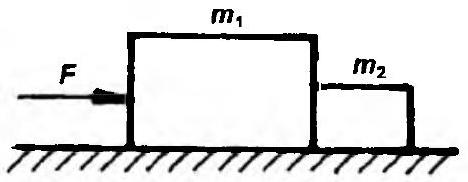
\includegraphics[width=0.4\linewidth]{images/2025_07_01_5b3ff9fa0d508c8e9f17g-033} Fig. 1.11\\

1.138. Un corp se mişcă uniform accelerat parcurgând distanța $d=120 \mathrm{~m}$. Prima jumătate de drum o parcurge în timpul $t_{1}=12 \mathrm{~s}$, iar cea de-a doua jumătate în timpul $t_{2}=8 \mathrm{~s}$. Să se afle accelerația corpului.\\ A) $1 \mathrm{~m} / \mathrm{s}$; B) $0,25 \mathrm{~m} / \mathrm{s}^{2}$; C) $0,2 \mathrm{~m} / \mathrm{s}$; D) $1,2 \mathrm{~m} / \mathrm{s}^{2}$; E) $4 \mathrm{~m} / \mathrm{s}^{2}$; F) $8 \mathrm{~m} / \mathrm{s}^{2}$\\ (Gabriela Tiriba)\\

1.139. Un corp este aruncat vertical în sus și revine pe pământ după un timp $t=2 \mathrm{~s}$. Sã se afle înălțimea la care s-a ridicat corpul ($g=9,8 \mathrm{~m} / \mathrm{s}^{2}$).\\ A) $19,6 \mathrm{~m}$; B) $9,8 \mathrm{~m}$; C) $39,2 \mathrm{~m}$; D) $4,9 \mathrm{~m}$; E) $29,4 \mathrm{~m}$; F) $16 \mathrm{~m}$.\\ (Gabriela Tiriba)\\

1.140. Pentru a menține în echilibru un corp pe un plan înclinat de unghi $\alpha=45^{\circ}$, trebuie aplicată corpului o forţă minimă normală pe plan de $n=2$ ori nai mare decât forța minimă orizontală. Să se calculeze coeficientul de frecare dintre corp şi plan.\\ A) $\frac{1}{7}$; B) $\frac{1}{2}$; C) $\frac{1}{\sqrt{2}}$; D) $\frac{\sqrt{2}+1}{7+\sqrt{2}}$; E) $\frac{\sqrt{3}}{2}$; F) $\frac{1}{2 \sqrt{2}-1}$. \\ (Gabriela Tiriba)\\

1.141. Un automobil face un viraj de rază $R=50 \mathrm{~m}$ cu viteza $v=36 \mathrm{~km} / \mathrm{h}$. Sã se afle coeficientul de frecare la alunecare minim pentru ca automobilul să nu alunece lateral ($g=9,8 \mathrm{~m} / \mathrm{s}^{2}$).\\ A) $0,1$; B) $0,03$; C) $0,2$; D) $0,5$; E) $0,9$; F) $0,04$.\\ (Gabriela Tiriba)\\

1.142. Un motor are puterea $P=98 \mathrm{~kW}$. Motorul este folosit pentru a ridica un corp cu masa $m=500 \mathrm{~kg}$ la o înălțime $h=18 \mathrm{~m}$. În cât timp va ridica motorul corpul respectiv?\\ A) $5 \mathrm{~s}$; B) $90 \mathrm{~s}$; C) $0,9 \mathrm{~s}$; D) $1 \mathrm{~min}$; E) $18 \mathrm{~s}$; F) $15 \mathrm{~min}$.\\ (Gabriela Tiriba)\\

1.143. Ce forţă constantă de frânare trebuie aplicatã unui tun de masă $m=400 \mathrm{~t}$ care se mişcă cu viteza $v_{0}=36 \mathrm{~km} / \mathrm{h}$, pentru a-l opri în timp de $20 \mathrm{~s}$?\\ A) $150 \mathrm{~N}$; B) $36 \mathrm{~N}$; C) $200 \mathrm{~kN}$; D) $300 \mathrm{~kN}$; E) $10 \mathrm{~N}$; F) $3 \mathrm{~kN}$.\\ (Gabriela Tiriba)\\

1.144. Un mobil se găseşte la momentul $t=0$ în punctul de coordonate $(2,0)$. Mobilul se mişcã în lungul axei $Ox$ conform legii de mişcare $x(t)=4 t^{2}+3 t+2$. La momentul $t=3 \mathrm{~s}$ de la începutul mişcării, viteza mobilului este:\\ A) $11 \mathrm{~m} / \mathrm{s}$; B) $27 \mathrm{~m} / \mathrm{s}$; C) $13 \mathrm{~m} / \mathrm{s}$; D) $17 \mathrm{~m} / \mathrm{s}$; E) $19 \mathrm{~m} / \mathrm{s}$; F) $37 \mathrm{~m} / \mathrm{s}$.\\ (Mihai Cristea)\\

1.145. Un corp este lansat cu aceeași viteză, o dată pe un plan înclinat de unghi $\alpha$ şi altă dată pe un plan orizontal, ambele caracterizate de acelaşi coeficient de frecare. Cunoscând că obiectul parcurge aceeaşi distanță până la oprire pe ambele plane, să se calculeze unghiul de frecare.\\ A) $\varphi=\alpha$; B) $\varphi=\frac{\alpha}{2}$; C) $\varphi=\frac{\pi-\alpha}{6}$; D) $\varphi=\frac{\pi}{4}$; E) $\varphi=\frac{\pi-\alpha}{2}$; F) $\varphi=\frac{2 \pi-\alpha}{4}$.\\ (Mihai Cristea)\\

1.146. Un corp este aruncat sub unghiul $\alpha$ în câmp gravitațional. Să se găseascā unghiul $\beta$ facut de viteză cu orizontala atunci când energia cinetică a corpului devine de $n$ ori mai mică decât energia cinetică inițială.\\ A) $\operatorname{tg} \beta=\sqrt{1+\frac{1}{n \cos ^{2} \alpha}}$; B) $\sin \beta=\frac{1}{\sqrt{n}}$; C) $\cos \beta=\sqrt{n} \cos \alpha$; D) $\operatorname{tg} \beta=\sqrt{1+\frac{1}{n \sin ^{2} \alpha}}$; E) $\sin \beta=\frac{1}{n}$; F) $\cos \beta=\sqrt{n} \sin \alpha$.\\ (Mihai Cristea)\\

1.147. Un corp cu masa $m=1 \mathrm{~kg}$ pleacă din repaus şi se mişcă fără frecare sub acțiunea forței reprezentată în Fig. 1.12. Când mobilul ajunge în punctul $x=8 \mathrm{~m}$, viteza lui va fi:\\ A) $4 \mathrm{~m} / \mathrm{s}$; B) $18 \mathrm{~m} / \mathrm{s}$; C) $36 \mathrm{~m} / \mathrm{s}$; D) $0 \mathrm{~m} / \mathrm{s}$; E) $24 \mathrm{~m} / \mathrm{s}$; F) $9 \mathrm{~m} / \mathrm{s}$.\\ (Mihai Cristea)\\ 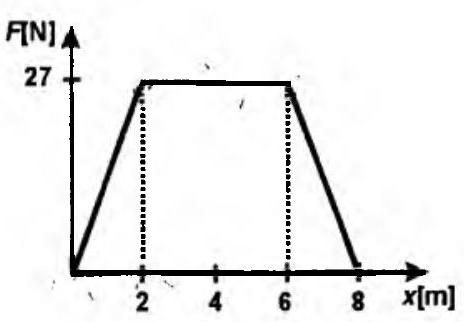
\includegraphics[width=0.4\linewidth]{images/2025_07_01_5b3ff9fa0d508c8e9f17g-035} Fig. 1.12\\

1.148.* Două corpuri de mase $m_{1}$ şi $m_{2}=n \cdot m_{1}(n>1)$ (Fig. 1. 13) alunecă fără frecare pe un profil cilindric de rază $R$, de la nivelul centrului profilului. În urma ciocnirii plastice a celor două corpuri, fracțiunea din energia potențială inițială transformată în căldură este:\\ A) $\frac{n}{n+1}$; B) $\left(\frac{n}{n+1}\right)^{2}$; C) $\frac{n-1}{n+1}$; D) $\left(\frac{n-1}{n+1}\right)^{2}$; E) $\frac{2 n}{n^{2}+1}$; F) $\frac{4 n}{(n+1)^{2}}$. \\ (Mihai Cristea)\\ 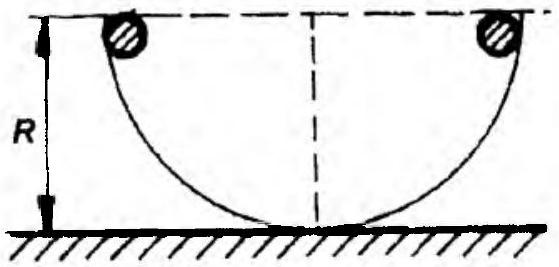
\includegraphics[width=0.4\linewidth]{images/2025_07_01_5b3ff9fa0d508c8e9f17g-035(1)} Fig. 1.13\\

1.149. Un corp masiv de masă $M$ este agățat de un fir inextensibil şi atârnă la distanţă $h_{1}$ de nivelul solului. Dacă se aruncă exact sub el, de la înălțimea $h_{2}$ fațã de sol un corp de masă $m$, acesta, în urma ciocnirii plastice, va ridica sistemul celor două corpuri pe o distanță $x$. Cunoscând viteza inițială $v_{0}$ cu care se aruncă corpul de masă $m$, să se determine cu cât se va modifica poziția corpului atârnat, înainte să cadă din nou.\\ A) $x=\left(\frac{m}{m+M}\right)^{2}\left(\frac{v_{0}^{2}}{2 g}-h_{1}+h_{2}\right)$; B) $x=\left(\frac{m}{m+M}\right) \cdot\left(\frac{v_{0}^{2}}{2 g}-h_{1}+h_{2}\right)$; C) $x=\left(\frac{m}{m+M}\right) \cdot\left(\frac{v_{0}^{2}}{2 g}-h_{1}-h_{2}\right)$; D) $x=\left(\frac{m}{m+M}\right) \cdot\left(\frac{v_{0}^{2}}{2 g}+h_{1}-h_{2}\right)$; E) $x=\left(\frac{m}{m+M}\right)^{2}\left(\frac{v_{0}^{2}}{2 g}+h_{1}-h_{2}\right)$; F) $x=\left(\frac{m}{m+M}\right)^{2}\left(\frac{v_{0}^{2}}{2 g}-h_{1}-h_{2}\right)$.\\ (Cristina Stan)\\

1.150. De la fereastra unui bloc turn, aflată la înălțimea de $25 \mathrm{~m}$ față de sol, un copil lasă să cadă o castană. După o secundă, el aruncă cu viteza inițială de $15 \mathrm{~m} / \mathrm{s}$ o a doua castană. Se întâlnesc cele două castane în drumul lor spre sol? La ce distanţă față de fereastră? ($\mathrm{g}=10 \mathrm{~m} / \mathrm{s}^{2}$).\\ A) Da, $d=18,4 \mathrm{~m}$; B) Nu, $d=15,2 \mathrm{~m}$; C) Da, $d=6,6 \mathrm{~m}$; D) Da, $d=4,9 \mathrm{~m}$; E) Da, $d=19,9 \mathrm{~m}$; F) Nu, $d=6,6 \mathrm{~m}$.\\ (Cristina Stan)\\

1.151. Un corp cu masa $m=10 \mathrm{~kg}$ este împins cu o forță orizontală de-a lungul unui plan înclinat care face unghiul $\alpha=45^{\circ}$ față de orizontală. Ce mărime trebuie să aibă această forţă pentru a produce o accelerație $a=1 / \sqrt{2} \mathrm{~m} / \mathrm{s}^{2}$ ştiind că valoarea coeficientului de frecare dintre corp şi planul înclinat este $\mu=0,2$? Se va considera accelerația gravitațională $g=10 \mathrm{~m} / \mathrm{s}^{2}$?\\ A) $75 \mathrm{~N}$; B) $100 \mathrm{~N}$; C) $450 \mathrm{~N}$; D) $162,5 \mathrm{~N}$; E) $55,7 \mathrm{~N}$; F) $90 \mathrm{~N}$.\\ (Cristina Stan)\\

1.152. O forță care acționează asupra unui obiect cu masa $m_{1}$ îi imprimă acestuia o accelerație $a_{1}$. Aceeaşi forță acționând asupra unei mase diferite, $m_{2}$, îi imprimă accelerația $a_{2}=2 a_{1}$. Dacă se lipesc cele două mase, ce accelerație va avea sistemul?\\ A) $3 a_{1}$; B) $\frac{1}{3} a_{1}$; C) $\frac{3}{2} a_{1}$; D) $\frac{2}{3} a_{1}$; E) $\frac{4}{3} a_{1}$; F) $\frac{5}{3} a_{1}$.\\ (Cristina Stan)\\

1.153.* Un automobil cu masa $m=800 \mathrm{~kg}$ staționează pe partea dreaptă a unui drum național. Un autocamion cu masa $M=1200 \mathrm{~kg}$ venind cu viteza $v=72 \mathrm{~km} / \mathrm{h}$ dintr-o curbă, nu îl observă în timp util astfel că se produce o coliziune în urma căreia ambele maşini rămân lipite. Pe ce distanţă se deplasează sistemul format din cele două maşini dacă coeficientul de frecare este $\mu=0,2$? Se consideră accelerația gravitațională $g=10 \mathrm{~m} / \mathrm{s}^{2}$.\\ A) $55 \mathrm{~m}$; B) $122 \mathrm{~m}$; C) $3,6 \mathrm{~m}$; D) $46,7 \mathrm{~m}$; E) $36 \mathrm{~m}$; F) $32 \mathrm{~m}$.\\ (Cristina Stan)\\

1.154. Două bile se deplasează una spre cealaltă, viteza bilei mai grele fiind de patru ori mai mare decât a celei mai uşoare. După ciocnirea perfect elastică, bila mai grea se opreşte. Raportul maselor bilelor este:\\ A) $1,25$; B) $1,5$; C) $2$; D) $2,5$; E) $3$; F) $4$.\\ (Constantin Neguţu)\\

1.155.* Două bărci se mişcă rectiliniu uniform cu aceeaşi viteză $v=0,6 \mathrm{~m} / \mathrm{s}$ pe direcții paralele, dar în sensuri opuse. Când bărcile ajung una în dreptul celeilalte, din prima se transferă în a doua un corp de masă $m=20 \mathrm{~kg}$. Ca urmare, a doua barcă își micşorează viteza până la $v_{2}=0,4 \mathrm{~m} / \mathrm{s}$. Masa celei de-a doua bărci este:\\ A) $80 \mathrm{~kg}$; B) $90 \mathrm{~kg}$; C) $110 \mathrm{~kg}$; D) $100 \mathrm{~kg}$; E) $140 \mathrm{~kg}$; F) $120 \mathrm{~kg}$.\\ (Constantin Neguțu)\\

1.156. Viteza $v_{0}$ cu care trebuie lansat orizontal un corp aflat la înălțimea $h$ pentru ca distanța parcursă pe orizontală să fie de $k$ ori mai mare decât $h$ este:\\ A) $\sqrt{\frac{g h k}{2}}$; B) $\sqrt{\frac{g h}{2 k}}$; C) $\frac{1}{k} \sqrt{\frac{g h}{2}}$; D) $\sqrt{\frac{h k}{2 g}}$; E) $\sqrt{\frac{g^{2} h k}{2}}$; F) $k \sqrt{\frac{g h}{2}}$.\\ (Constantin Neguțu)\\

1.157.* Un corp alunecă pe un plan înclinat de unghi $\alpha=45^{\circ}$ cu planul orizontal şi coeficient de frecare $\mu=0,2$ de la o înălțime $h=12 \mathrm{~m}$. La baza planului, corpul se ciocneşte perfect elastic de un perete aşezat perpendicular pe acesta (Fig. 1.14). După ciocnire, corpul va ajunge la înălțimea:\\ A) $8 \mathrm{~m}$; B) $9 \mathrm{~m}$; C) $8,5 \mathrm{~m}$; D) $6 \mathrm{~m}$; E) $4 \mathrm{~m}$; F) $10 \mathrm{~m}$.\\ (Constantin Neguțu)\\ 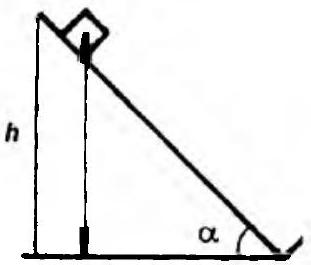
\includegraphics[width=0.4\linewidth]{images/2025_07_01_5b3ff9fa0d508c8e9f17g-037} Fig. 1.14\\

1.158. O minge de tenis de câmp cu masa de $50 \mathrm{~g}$ şi viteza de $180 \mathrm{~km} / \mathrm{h}$ loveşte terenul perfect elastic sub unghiul de $60^{\circ}$ față de verticală. Durata impactului este de $10^{-3} \mathrm{~s}$. Forța cu care mingea loveşte terenul este:\\ A) $1750 \mathrm{~N}$; B) $2500 \mathrm{~N}$; C) $3000 \mathrm{~N}$; D) $1500 \mathrm{~N}$; E) $2000 \mathrm{~N}$; F) $4000 \mathrm{~N}$.\\ (Constantin Neguțu)\\

1.159.* Să se afle masa Soarelui, cunoscând viteza liniară de rotație a Pământului în jurul Soarelui, $v=30 \mathrm{~km} / \mathrm{s}$, raza orbitei Pământului, presupusă circulară, $R=1,5 \cdot 10^{10} \mathrm{~km}$ şi constanta atracției universale, $k=6,67 \cdot 10^{-11} \mathrm{Nm}^{2} / \mathrm{kg}^{2}$.\\ A) $2 \cdot 10^{30} \mathrm{~kg}$; B) $2 \cdot 10^{32} \mathrm{~kg}$; C) $2 \cdot 10^{27} \mathrm{~kg}$; D) $1,2 \cdot 10^{30} \mathrm{~kg}$; E) $2 \cdot 10^{34} \mathrm{~kg}$; F) $2 \cdot 10^{24} \mathrm{~kg}$.\\ (Constantin Neguțu)\\

1.160. Variația energiei cinetice a unui corp asupra căruia acționează un sistem de forţe este egalã cu:\\ A) variația energiei potențiale; B) zero; C) lucrul mecanic efectuat de forța rezultantă ce acționează asupra corpului în timpul acestei variații; D) lucrul mecanic efectuat de câmpul gravitațional; E) momentul forței rezultante față de centrul de masă al corpului; F) impulsul forței rezultante.\\ (Constantin Neguțu)\\

1.161.* În cazul ciocnirii perfect plastice a două corpuri se conservă:\\ A) energia cinetică a sistemului; B) energia potențială a sistemului; C) impulsul sistemului; D) energia cinetică şi impulsul sistemului; E) impulsul şi energia potențială a sistemului; F) energia potențială, energia cinetică şi impulsul sistemului.\\ (Constantin Neguțu)\\

1.162.* Un corp cade liber de la înălţimea de $100 \mathrm{~m}$. După $4 \mathrm{~s}$ de cădere este ciocnit plastic de un corp cu aceeaşi masă, având viteza de $20 \mathrm{~m} / \mathrm{s}$ orientată orizontal. Distanța parcursă pe orizontală față de locul ciocnirii este ($\mathrm{g}=10 \mathrm{~m} / \mathrm{s}^{2}$):\\ A) $82 \mathrm{~m}$; B) $0,82 \mathrm{~m}$; C) $0 \mathrm{~m}$; D) $18,2 \mathrm{~m}$; E) $8,2 \mathrm{~m}$; F) $10 \mathrm{~m}$.\\ (Constantin Neguţu)\\

1.163.* Doi motociclişti aleargă cu o mişcare uniformă pe același cerc pornind în același moment din acelaşi punct. Vitezele lor sunt $v_{1}=54 \mathrm{~km} / \mathrm{h}$ şi $v_{2}=43,2 \mathrm{~km} / \mathrm{h}$. Neglijând mişcarea accelerată de la pornire, numărul de rotații după care unul îl prinde pe celălalt din urmă în punctul de plecare este:\\ A) $1$; B) $2$; C) $3$; D) $4$; E) $5$; F) $6$.\\ (Constantin Neguțu)\\

1.164.* De la o înălțime $h_{0}$ față de un plan orizontal se lasă liberă, fară viteză inițială, o bilă. Bila loveşte planul cu viteza $v_{0}$ şi se întoarce cu viteza $v_{1}=e v_{0}$ ($v_{0}$ şi $v_{1}$ în valori absolute). Durata totală a mişcării bilei până ce aceasta se opreşte este:\\ A) $\sqrt{\frac{2 h_{0}}{g}} \frac{1+e}{1-e}$; B) $\sqrt{\frac{2 h_{0}}{g}} \frac{e}{1-e}$; C) $\frac{1}{2} \sqrt{\frac{2 h_{0}}{g}} \frac{e}{1-e}$; D) $2 \sqrt{\frac{2 h_{0}}{g}} \frac{e}{1+e}$; E) $2 \sqrt{\frac{2 h_{0}}{g}} \frac{1+e}{1-e}$; F) $\sqrt{\frac{2 h_{0}}{g}} \frac{e}{1+e}$.\\ (Constantin Neguțu)\\

1.165. Un tren de masă $m=1200 \mathrm{~t}$ are o viteză inițială $v=72 \mathrm{~km} / \mathrm{h}$. Coeficientul de frecare dintre tren şi şine este $\mu=0,05$. Ce forţă de frânare trebuie aplicată pentru ca trenul să fie oprit în $20 \mathrm{~s}$ de la oprirea motorului electric al locomotivei (se consideră $g=10 \mathrm{~m} / \mathrm{s}^{2}$)?\\ A) $6 \cdot 10^{5} \mathrm{~N}$; B) $3 \cdot 10^{6} \mathrm{~N}$; C) $8 \cdot 10^{4} \mathrm{~N}$; D) $5 \cdot 10^{5} \mathrm{~N}$; E) $4,5 \cdot 10^{6} \mathrm{~N}$; F) $8,3 \cdot 10^{5} \mathrm{~N}$.\\ (Cristian Toma)\\

1.166.* Un corp de masă $m=30 \mathrm{~kg}$ se deplasează cu viteza $v=30 \mathrm{~m} / \mathrm{s}$. Pe acest corp este pus un corp de masă $m^{\prime}$, după acest impact corpurile deplasându-se cu viteza $v^{\prime}=10 \mathrm{~m} / \mathrm{s}$. Care este masa $m^{\prime}$ a celui de-al doilea corp?\\ A) $20 \mathrm{~kg}$; B) $60 \mathrm{~kg}$; C) $35 \mathrm{~kg}$; D) $47 \mathrm{~kg}$; E) $52 \mathrm{~kg}$; F) $74 \mathrm{~kg}$.\\ (Cristian Toma)\\

1.167. În ce condiţii vitezele relative $\vec{v}_{1}$ şi $\vec{v}_{2}$ ale celor două şenile ale unui tractor considerate în raport cu centrul tractorului sunt egale în modul satisfăcând relația $\left|\vec{v}_{1}\right|=\left|\vec{v}_{2}\right|=|\vec{a}|$ (unde $\vec{a}$ este un vector cunoscut de modul nenul) astfel ca centrul tractorului să rămână în repaus?\\ A) $\vec{v}_{1}=\vec{a}, \vec{v}_{2}=\vec{a}$; B) $\vec{v}_{1}=\vec{a}, \vec{v}_{2}=\vec{a} / 2$; C) $\vec{v}_{1}=-\vec{a}, \vec{v}_{2}=\vec{a}$; D) $\vec{v}_{1}=-\vec{a}, \vec{v}_{2}=-\vec{a} / 2$; E) $\vec{v}_{1}=-\vec{a}, \vec{v}_{2}=-\vec{a}$; F) $\vec{v}_{1}=-\vec{a}, \vec{v}_{2}=\vec{a} / 2$.\\ (Cristian Toma)\\

1.168. Să se calculeze coeficientul de frecare $\mu$ dintre un automobil de $500 \mathrm{~kg}$ şi sol dacă pentru a se deplasa cu viteza de $108 \mathrm{~km} / \mathrm{h}$ aceasta foloseşte o putere de $3 \times 10^{4} \mathrm{~W}$ (se consideră $g=10 \mathrm{~m} / \mathrm{s}^{2}$).\\ A) $\mu=0,1$; B) $\mu=0,01$; C) $\mu=0,2$; D) $\mu=0,25$; E) $\mu=0,15$; F) $\mu=0,02$.\\ (Cristian Toma)\\

1.169. La o curbă de rază $R=49 \mathrm{~m}$ drumul a fost înclinat în raport cu suprafața orizontală la unghiul $\alpha=\operatorname{arctg} 0,1$. Considerând $g=10 \mathrm{~m} / \mathrm{s}^{2}$, să se afle pentru ce viteză a fost proiectat drumul respectiv.\\ A) $v=7 \mathrm{~m} / \mathrm{s}$; B) $v=1 \mathrm{~m} / \mathrm{s}$; C) $v=49 \mathrm{~m} / \mathrm{s}$; D) $v=14 \mathrm{~m} / \mathrm{s}$; E) $v=1,4 \mathrm{~m} / \mathrm{s}$; F) $v=4,9 \mathrm{~m} / \mathrm{s}$.\\ (Cristian Toma)\\

1.170.* Un ceasornic cu cadran este pornit la ora 12 (când orarul, minutarul şi secundarul sunt aliniate). La ce unghi cu axa ce uneşte centrul cadranului cu poziția corespunzătoare orei 12 se întâlnesc din nou, pentru prima oară, secundarul şi minutarul?\\ A) $\frac{\pi}{2} \mathrm{rad}$; B) $\frac{\pi}{4} \mathrm{rad}$; C) $\frac{\pi}{59} \mathrm{rad}$; D) $\frac{\pi}{60} \mathrm{rad}$; E) $\frac{2 \pi}{59} \mathrm{rad}$; F) $\frac{2 \pi}{60} \mathrm{rad}$.\\ (Cristian Toma)\\

1.171.* Un corp lansat cu viteza $v=10 \mathrm{~m} / \mathrm{s}$ de la sol, sub unghiul $\alpha$ față de orizontală, revine la sol la distanța de $5 \sqrt{3} \mathrm{~m}$ față de poziția de plecare. Sã se afle unghiul $\alpha$ (se consideră $g=10 \mathrm{~m} / \mathrm{s}^{2}$).\\ A) $\frac{\pi}{2}$; B) $\frac{\pi}{4}$; C) $\frac{\pi}{3}$; D) $\frac{\pi}{6}$; E) $\frac{\pi}{8}$; F) $\frac{\pi \sqrt{3}}{2}$.\\ (Cristian Toma)\\

1.172.* Un corp de masă $m$ este aruncat de la sol din punctul O cu viteza inițială $v$ sub un unghi $\alpha$ în raport cu o axă $Ox$ conținută în planul solului, astfel încât proiecția poziției sale pe sol să aparțină permanent acestei axe $Ox$. Acest corp ajunge la sol în punctul M. Să se afle valoarea unghiului $\alpha$ astfel încât distanța OM (în modul) să fie maximă.\\ A) $\alpha \in\left\{\frac{\pi}{4}\right\}$; B) $\alpha \in\left\{\frac{\pi}{2}, \pi\right\}$; C) $\alpha \in\left\{\frac{\pi}{4}, \frac{3 \pi}{4}\right\}$; D) $\alpha \in\left\{\frac{\pi}{4},-\frac{\pi}{4}\right\}$; E) $\alpha \in\left\{\frac{3 \pi}{4}\right\}$; F) $\alpha \in\left\{-\frac{\pi}{4}\right\}$.\\ (Cristian Toma)\\

1.173. Metroul parcurge distanța dintre două stații consecutive în $2 \mathrm{~min} 20 \mathrm{~s}$, realizând o mişcare uniform accelerată urmată de una uniformă și apoi de una uniform încetinită. Dacă accelerațiile inițială și finală sunt egale în valoare absolută, $|a|=1 \mathrm{~m} / \mathrm{s}^{2}$, şi viteza maximă la care ajunge trenul este $v_{m}=90 \mathrm{~km} / \mathrm{h}$ să se determine distanța dintre cele două stații.\\ A) $2,5 \mathrm{~km}$; B) $2225 \mathrm{~m}$; C) $2875 \mathrm{~m}$; D) $1,25 \mathrm{~km}$; E) $12500 \mathrm{~m}$; F) $22,5 \mathrm{~km}$.\\ (Ion Gurgu)\\

1.174. Un corp este aruncat pe verticală în sus cu viteza inițială $v_{0}=10 \mathrm{~m} / \mathrm{s}$. Peste cât timp acesta se va găsi la înălțimea $h=10 \mathrm{~m}$?\\ A) $1 \mathrm{~s}$; B) imposibil; C) $10 \mathrm{~s}$; D) $1,5 \mathrm{~s}$; E) $1 \mathrm{~h}$; F) $0,5 \mathrm{~s}$.\\ (Ion Gurgu)\\

1.175. Un glonte cu masa $m=25 \mathrm{~g}$ pătrunde într-o scândură pe distanța $d=5 \mathrm{~cm}$. Dacă viteza inițială a glontelui este $v_{0}=500 \mathrm{~m} / \mathrm{s}$, ce impuls ar primi o scândură identică, de grosime $2 \mathrm{~cm}?$\\ A) $2 \mathrm{~kg}$; B) $2,8 \mathrm{Ns}$; C) $5,6 \mathrm{Ns}$; D) nu primeşte impuls; E) $1,4 \mathrm{Nm}$; F) $1,4 \mathrm{Ns}$.\\ (Ion Gurgu)\\

1.176. De capetele unui fir trecut peste un scripete sunt legate două corpuri cu masele $m_{1}=10 \mathrm{~g}$ şi $m_{2}=50 \mathrm{~g}$. Dacă sistemul este lăsat liber, să se calculeze înălțimea maximă la care se ridică masa $m_{1}$, cunoscând $h_{2}=50 \mathrm{~cm}$ (Fig. 1.15). Se consideră $g=10 \mathrm{~m} / \mathrm{s}^{2}$.\\ A) $5 / 6 \mathrm{~m}$; B) $6 / 5 \mathrm{~m}$; C) $1 \mathrm{~m}$; D) nu se ridică; E) $0,5 \mathrm{~m}$; F) $1,5 \mathrm{~m}$.\\ (Ion Gurgu)\\ 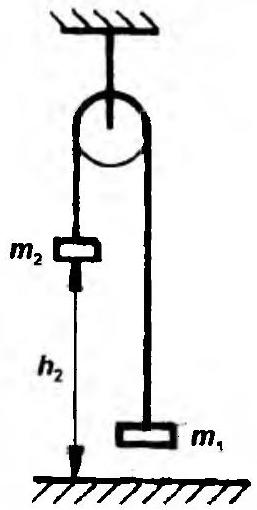
\includegraphics[width=0.4\linewidth]{images/2025_07_01_5b3ff9fa0d508c8e9f17g-042} Fig. 1.15\\

1.177. Un corp este aruncat cu viteza inițială $v_{0}=6 \mathrm{~m} / \mathrm{s}$, pe un plan înclinat de unghi $\alpha=45^{\circ}$. Cunoscând că mişcarea se face cu frecare şi timpul de coborâre este de 3 ori mai mare decât la urcare, să se determine înălțimea până la care a urcat corpul.\\ A) $1 \mathrm{~m}$; B) $1,1 \mathrm{~m}$; C) $0,9 \mathrm{~m}$; D) imposibil; E) $1,5 \mathrm{~m}$; F) $0,1 \mathrm{~m}$.\\ (Ion Gurgu)\\

1.178.* Un corp coboară liber, fără frecare, pe un plan înclinat şi de la baza acestuia îşi continuă mişcarea pe o traiectorie circulară de rază $R=1 \mathrm{~m}$ (Fig. 1.16). Dacă corpul coboară de la înălțimea $h=2 R$, să se determine înălțimea $h_{1}$ la care ajunge corpul pe traiectoria circulară.\\ A) $1,0 \mathrm{~m}$; B) $0,1 \mathrm{~m}$; C) imposibil; D) $1,61 \mathrm{~m}$; E) $2,0 \mathrm{~m}$; F) $0,5 \mathrm{~m}$.\\ (Ion Gurgu)\\ 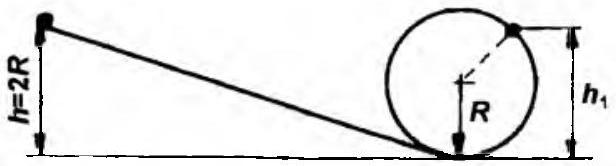
\includegraphics[width=0.4\linewidth]{images/2025_07_01_5b3ff9fa0d508c8e9f17g-042(1)} Fig. 1.16\\

1.179. Din vârful unui turn cu înălțimea $h=60 \mathrm{~m}$ este aruncat în sus un corp cu viteza inițială $v_{0}=20 \mathrm{~m} / \mathrm{s}$. Cu ce viteză va atinge corpul solul? ($g=10 \mathrm{~m} / \mathrm{s}^{2}$).\\ A) $30 \mathrm{~m} / \mathrm{s}$; B) $60 \mathrm{~m} / \mathrm{s}$; C) $40 \mathrm{~m} / \mathrm{s}$; D) $120 \mathrm{~m} / \mathrm{s}$; E) $20 \mathrm{~m} / \mathrm{s}$; F) $80 \mathrm{~m} / \mathrm{s}$.\\ (Marcel Dobre)\\

1.180. Un corp este aruncat fără frecare pe un plan înclinat. La $1 \mathrm{~s}$, respectiv $2 \mathrm{~s}$ din momentul aruncării, corpul se află la distanța de $0,3 \mathrm{~m}$ de punctul de aruncare. Să se calculeze viteza inițială a corpului.\\ A) $4,5 \mathrm{~m} / \mathrm{s}$; B) $45 \mathrm{~m} / \mathrm{s}$; C) $0,45 \mathrm{~m} / \mathrm{s}$; D) $0,9 \mathrm{~m} / \mathrm{s}$; E) $1,5 \mathrm{~m} / \mathrm{s}$; F) $2 \mathrm{~m} / \mathrm{s}$.\\ (Marcel Dobre)\\

1.181.* O piatră este aruncată cu $v_{0}=20 \mathrm{~m} / \mathrm{s}$ sub unghi $\alpha=60^{\circ}$ cu orizontala. Să se calculeze raza de curbură în punctul situat la înălțimea maximă. ($g=10 \mathrm{~m} / \mathrm{s}^{2}$).\\ A) $1 \mathrm{~m}$; B) $10 \mathrm{~m}$; C) $40 \mathrm{~m}$; D) $18 \mathrm{~m}$; E) $20 \mathrm{~m}$; F) $5 \mathrm{~m}$.\\ (Marcel Dobre)\\

1.182. O porţiune de şosea prezintă o pantă de $0,05$. Pe această şosea un automobil cu masa $m=150 \mathrm{~kg}$ coboară uniform având motorul decuplat, cu viteza de $10 \mathrm{~m} / \mathrm{s}$. Care trebuie să fie puterea motorului pentru ca automobilul să urce นniform aceeaşi pantã cu aceeaşi viteză? ($g=10 \mathrm{~m} / \mathrm{s}^{2}$).\\ A) $15000 \mathrm{~W}$; B) $1500 \mathrm{~W}$; C) $3500 \mathrm{~W}$; D) $12000 \mathrm{~W}$; E) $25000 \mathrm{~W}$; F) $10000 \mathrm{~W}$.\\ (Marcel Dobre)\\

1.183.* O piatră cu masa $m=0,2 \mathrm{~kg}$ este aruncată oblic pe o suprafață orizontală şi revine pe aceeaşi suprafață la o distanță $S=5 \mathrm{~m}$ de locul aruncării după $t=1 \mathrm{~s}$. Dacă se neglijează frecarea, să se afle lucrul mecanic necesar pentru efectuarea aruncării. ($g=10 \mathrm{~m} / \mathrm{s}^{2}$).\\ A) $10 \mathrm{~J}$; B) $15 \mathrm{~J}$; C) $25 \mathrm{~J}$; D) $100 \mathrm{~J}$; E) $60 \mathrm{~J}$; F) $5 \mathrm{~J}$.\\ (Marcel Dobre)\\

1.184.* Sub acțiunea unui impuls inițial o greutate legată cu un fir de tavan descrie un cerc situat în plan orizontal la o distanță de $1,5 \mathrm{~m}$ de tavan. Care este frecvența rotațiilor greutății? ($g=10 \mathrm{~m} / \mathrm{s}^{2}$).\\ A) $0,91 \mathrm{~s}^{-1}$; B) $0,41 \mathrm{~s}^{-1}$; C) $0,5 \mathrm{~s}^{-1}$; D) $1,14 \mathrm{~s}^{-1}$; E) $2,4 \mathrm{~s}^{-1}$; F) $3,2 \mathrm{~s}^{-1}$.\\ (Marcel Dobre)\\

1.185. Sub acțiunea unei forțe $F_{1}=9 \mathrm{~N}$, un punct material se mişcă cu accelerația $a_{1}=3 \mathrm{~m} / \mathrm{s}^{2}$. Cu ce accelerație se va mişca acesta sub acțiunea unei forțe $F_{2}=6 \mathrm{~N}$?\\ A) $1 \mathrm{~m} / \mathrm{s}^{2}$; B) $2 \mathrm{~m} / \mathrm{s}^{2}$; C) $5 \mathrm{~m} / \mathrm{s}^{2}$; D) $2,5 \mathrm{~m} / \mathrm{s}^{2}$; E) $-3 \mathrm{~m} / \mathrm{s}^{2}$; F) $-5 \mathrm{~m} / \mathrm{s}^{2}$.\\ (Marin Cilea)\\

1.186. O minge cu masa $m=0,2 \mathrm{~kg}$ a căpătat, după lovire, o viteză $v=15 \mathrm{~m} / \mathrm{s}$. Dacă durata lovirii a fost $\Delta t=10^{-2} \mathrm{~s}$, să se afle forța medie de lovire.\\ A) $300 \mathrm{~N}$; B) $1 \mathrm{~kN}$; C) $500 \mathrm{~N}$; D) $0,2 \mathrm{kN}$; E) $125,5 \mathrm{~N}$; F) $15 \mathrm{~kN}$.\\ (Marin Cilea)\\

1.187. Un camion cu masa $m=10 \mathrm{t}$ porneşte cu accelerația $a=0,55 \mathrm{~m} / \mathrm{s}^{2}$. Cunoscând că forțele de frecare (de rezistență) au valoarea de $500 \mathrm{~N}$, să se afle forța de tracțiune a motorului.\\ A) $2 \mathrm{~kN}$; B) $2,5 \mathrm{kN}$; C) $10 \mathrm{~kN}$; D) $6 \mathrm{~kN}$; E) $10^{3} \mathrm{~N}$; F) $500 \mathrm{~N}$.\\ (Marin Cilea)\\

1.188. O săniuță coboară liber un deal de lungime $l=50 \mathrm{~m}$ într-un timp $t=10 \mathrm{~s}$. Cu ce viteză a ajuns ea la baza dealului?\\ A) $3 \mathrm{~m} / \mathrm{s}$; B) $1 \mathrm{~m} / \mathrm{s}$; C) $4,5 \mathrm{~m} / \mathrm{s}$; D) $50 \mathrm{~m} / \mathrm{s}$; E) $25 \mathrm{~m} / \mathrm{s}$; F) $10 \mathrm{~m} / \mathrm{s}$.\\ (Marin Cilea)\\

1.189. Un corp aruncat vertical în sus a revenit pe pământ după $\tau=10 \mathrm{~s}$. Cu ce viteză inițială a fost aruncat corpul? ($g=10 \mathrm{~m} / \mathrm{s}^{2}$).\\ A) $10 \mathrm{~m} / \mathrm{s}$; B) $20 \mathrm{~m} / \mathrm{s}$; C) $50 \mathrm{~m} / \mathrm{s}$; D) $25 \mathrm{~m} / \mathrm{s}$; E) $100 \mathrm{~m} / \mathrm{s}$; F) $15 \mathrm{~m} / \mathrm{s}$.\\ (Marin Cilea)\\

1.190.* Un autoturism cu masa $m=1 \mathrm{~t}$ merge cu viteza $v=10 \mathrm{~m} / \mathrm{s}$ peste un pod convex, cu raza de curbură $R=100 \mathrm{~m}$. Ce apăsare exercită autoturismul asupra podului în punctul superior? ($g=10 \mathrm{~m} / \mathrm{s}^{2}$).\\ A) $1 \mathrm{~kN}$; B) $10^{4} \mathrm{~N}$; C) $280,6 \mathrm{~N}$; D) $0 \mathrm{~N}$; E) $9 \mathrm{~kN}$; F) $500 \mathrm{~N}$.\\ (Marin Cilea)\\

1.191. Un resort a fost comprimat cu $x=4 \mathrm{~cm}$ sub acțiunea unei forțe $F=25 \mathrm{~N}$. Calculați energia potențială a resortului.\\ A) $10 \mathrm{~J}$; B) $5 \mathrm{~J}$; C) $1 \mathrm{~J}$; D) $0,5 \mathrm{~J}$; E) $25 \mathrm{~J}$; F) $8 \mathrm{~J}$.\\ (Marin Cilea)\\

1.192.* Un corp cu masa $m_{1}=0,5 \mathrm{~kg}$ şi viteza $v_{1}=10 \mathrm{~m} / \mathrm{s}$ loveşte un alt corp care se mişcă spre el pe aceeaşi direcție. După ciocnire corpurile se opresc. Calculați modulul impulsului pentru cel de-al doilea corp.\\ A) $10 \mathrm{~kg} \cdot \frac{\mathrm{~m}}{\mathrm{~s}}$; B) $3 \mathrm{~N} \cdot \mathrm{~s}$; C) $5 \mathrm{~N} \cdot \mathrm{~s}$; D) $4 \frac{\mathrm{~kg} \cdot \mathrm{~m}}{\mathrm{~s}}$; E) $0,5 \mathrm{~N} \cdot \mathrm{~s}$; F) $12,3 \mathrm{~N} \cdot \mathrm{~m}$.\\ (Marin Cilea)\\

1.193. Impulsul unui corp este $p=10 \mathrm{~N} \cdot \mathrm{~s}$, iar energia cinetică $E_{c}=10 \mathrm{~J}$. Să se afle masa corpului.\\ A) $1 \mathrm{~kg}$; B) $3 \mathrm{~kg}$; C) $5 \mathrm{~kg}$; D) $7 \mathrm{~kg}$; E) $9 \mathrm{~kg}$; F) $11 \mathrm{~kg}$.\\ (Marin Cilea)\\

1.194. Un corp cu masa $m=1 \mathrm{~kg}$, fără viteză inițială, coboară fără frecare pe un plan înclinat de înălțime $h=5 \mathrm{~m}$. Ajungând la baza planului, corpul se deplasează cu frecare pe o suprafață plană orizontală până se opreşte. Să se calculeze timpul total de mişcare pe planul înclinat şi pe cel orizontal. Se dau: $\alpha=30^{\circ}, \mu=0,2, g=10 \mathrm{~m} / \mathrm{s}^{2}$.\\ A) $7\mathrm{~s}$; B) $14 \mathrm{~s}$; C) $2 \mathrm{~s}$; D) $5 \mathrm{~s}$; E) $6 \mathrm{~s}$; F) $4,2 \mathrm{~s}$.\\ (Tatiana Pop)\\

1.195. Un punct material este lansat în sus de-a lungul unui plan înclinat care realizează unghiul $\alpha=45^{\circ}$ cu orizontala, cu viteza inițială $v_{0}=6 \mathrm{~m} / \mathrm{s}$. Mişcarea se face cu frecare, coeficientul de frecare la alunecare între corp şi planul înclinat fiind $\mu=0,2$. Dacă din punctul de înălțime maximă, corpul coboară cu viteza inițială nulă, de câte ori este mai mare timpul de coborâre până la baza planului față de timpul de urcare? Se dă $g=10 \mathrm{~m} / \mathrm{s}^{2}$. \\ A) $1,22$; B) $1,4$; C) $2$; D) $5$; E) $6$; F) $2,32$.\\ (Tatiana Pop)\\

1.196. Un corp cade liber de la o înălțime de $490 \mathrm{~m}$. Ce spațiu străbate el în ultima secundă a mişcării? ($g=9,80 \mathrm{~m} / \mathrm{s}^{2}$).\\ A) $98 \mathrm{~m}$; B) $93,1 \mathrm{~m}$; C) $9,8 \mathrm{~m}$; D) $108 \mathrm{~m}$; E) $100 \mathrm{~m}$; F) $88,6 \mathrm{~m}$.\\ (Tatiana Pop)\\

1.197. Un automobil cu masa $1000 \mathrm{~kg}$ porneşte din repaus şi ajunge la viteza de $30 \mathrm{~m} / \mathrm{s}$ după ce parcurge $500 \mathrm{~m}$ pe un drum orizontal. Să se calculeze forţa de tracțiune a motorului, dacă forța de frecare este de $200 \mathrm{~N}$.\\ A) $F=1000 \mathrm{~N}$; B) $F=1050 \mathrm{~N}$; C) $F=1100 \mathrm{~N}$; D) $F=900 \mathrm{~N}$; E) $F=1150 \mathrm{~N}$; F) $F=1350 \mathrm{~N}$.\\ (Tatiana Pop)\\

1.198.* Un corp se mişcă uniform pe un cerc de rază $R=10 \mathrm{~m}$, sub acțiunea unei forțe centripete $F=100 \mathrm{~N}$. Lucrul mecanic efectuat de această forță într-o perioadă a mişcării este:\\ A) $L=2000 \pi \mathrm{~J}$; B) $L=1000 \pi \mathrm{~J}$; C) $L=0 \mathrm{~J}$; D) $L=3000 \pi \mathrm{~J}$; E) $L=1000 \mathrm{~J}$; F) $L=100 \pi \mathrm{~J}$.\\ (Tatiana Pop)\\

1.199. Firul $AB$ inextensibil și de masă neglijabilă, fixat în $A$, are prins în $B$ un corp cu masa de $2 \mathrm{~kg}$. Se scoate firul din poziția de echilibru, astfel încât formează cu verticala unghiul de $60^{\circ}$. Se lasă corpul liber. Tensiunea din fir, când acesta face cu verticala unghiul de $30^{\circ}$ ($g=10 \mathrm{~m} / \mathrm{s}^{2}$), este:\\ A) $F=1,7 \mathrm{~N}$; B) $F=73,1 \mathrm{~N}$; C) $F=20 \mathrm{~N}$; D) $F=31,9 \mathrm{~N}$; E) $F=40 \mathrm{~N}$; F) $24,5 \mathrm{~N}$.\\ (Tatiana Pop)\\

1.200. Pentru a deplasa un corp în sus pe un plan înclinat cu unghiul de $45^{\circ}$ este necesară o forță tangențială minimă de $30 \mathrm{~N}$, iar pentru a-l menține în repaus, forța tangențială minimă este de $15 \mathrm{~N}$, îndreptată în acelaşi sens ca şi prima. Care este coeficientul de frecare dintre corp şi planul înclinat?\\ A) $0,5$; B) $0,1$; C) $3 / 4$; D) $1 / 3$; E) $0,6$; F) $0,24$.\\ (Tatiana Pop)\\

1.201.* Un corp execută o mişcare oscilatorie armonică. Pentru a îndepărta corpul din poziția de repaus până la elongația maximă se cheltuieşte un lucru mecanic $L=0,5 \mathrm{~J}$. Forța elastică care acționează asupra corpului în acest punct este $F=2,5 \mathrm{~N}$. Care este amplitudinea mişcării oscilatorii?\\ A) $0,25 \mathrm{~m}$; B) $0,3 \mathrm{~m}$; C) $0,35 \mathrm{~m}$; D) $0,4 \mathrm{~m}$; E) $0,5 \mathrm{~m}$; F) $0,55 \mathrm{~m}$.\\ (Tatiana Pop)\\

1.202. Ecuația mişcării unui mobil este $x=2+6 t-t^{2}$ (valorile exprimate în Sistemul Internațional). După ce timp viteza mobilului este egală cu o treime din viteza inițială ?\\ A) $1 / 3 \mathrm{~s}$; B) $4 \mathrm{~s}$; C) $1 \mathrm{~s}$; D) $0,5 \mathrm{~s}$; E) $2 \mathrm{~s}$; F) $3 \mathrm{~s}$.\\ (Mona Mihăilescu)\\

1.203. Un corp parcurge în mişcare uniform accelerată cu viteza inițială $v_{0}$ o distanță $s=96 \mathrm{~m}$. Prima jumătate o parcurge în $t_{1}=8 \mathrm{~s}$, iar cealaltă jumătate în $t_{2}=4 \mathrm{~s}$. Se cere accelerația corpului.\\ A) $3,2 \mathrm{~m} / \mathrm{s}^{2}$; B) $1,4 \mathrm{~m} / \mathrm{s}^{2}$; C) $2,4 \mathrm{~m} / \mathrm{s}^{2}$; D) $5 \mathrm{~m} / \mathrm{s}^{2}$; E) $6 \mathrm{~m} / \mathrm{s}^{2}$; F) $1 \mathrm{~m} / \mathrm{s}^{2}$.\\ (Mona Mihǎilescu)\\

1.204. Un corp de masă $m=4 \mathrm{~kg}$ este acționat cu o forță $F=60 \mathrm{~N}$ orientată pe verticală în sus. Cu ce accelerație se mişcă corpul? Se neglijează frecarea. Se consideră $g=10 \mathrm{~m} / \mathrm{s}^{2}$\\ A) $25 \mathrm{~m} / \mathrm{s}^{2}$ sus; B) $5 \mathrm{~m} / \mathrm{s}^{2}$ jos; C) $400 \mathrm{~m} / \mathrm{s}^{2}$ sus; D) $25 \mathrm{~m} / \mathrm{s}^{2}$ jos; E) $5 \mathrm{~m} / \mathrm{s}^{2}$ sus; F) $20 \mathrm{~m} / \mathrm{s}^{2}$ jos.\\ (Mona Mihăilescu)\\

1.205. Un resort aflat pe un plan orizontal este fixat la un capăt, iar la celălalt e legat un corp de masă $m$. La momentul inițial resortul e netensionat, se imprimă corpului $m$ viteza $v_{0}$ în sensul destinderii resortului. Dacă se cunoaşte constanta elastică $K$, se cere deformația maximă în lipsa frecărilor.\\ A) $\frac{m v_{0}}{K}$; B) $\frac{\sqrt{m v_{0}}}{K}$; C) $v_{0} \sqrt{\frac{m}{K}}$; D) $v_{0} \sqrt{\frac{K}{m}}$; E) $\frac{v_{0}}{m} \sqrt{K}$; F) $v_{0} \sqrt{\frac{2 m}{K}}$.\\ (Mona Mihăilescu)\\

1.206.* Acele unui ceasornic au lungimile $l_{1}=3 \mathrm{~cm}$ (orarul) şi $l_{2}=4,5 \mathrm{~cm}$ (minutarul). Care este raportul vitezelor periferice $v_{1} / v_{2}$ ale celor două ace?\\ A) $2 / 3$; B) $8$; C) $1 / 3$; D) $1/18$; E) $1 / 90$; F) $2 / 30$.\\ (Mona Mihăilescu)\\

1.207. Un corp cu greutatea de $10 \mathrm{~N}$ cade liber un sfert de minut. Care este variația impulsului corpului neglijând frecările ($g=10 \mathrm{~m} / \mathrm{s}^{2}$ )?\\ A) $250 \mathrm{kgm} / \mathrm{s}$; B) $15 \mathrm{kgm} / \mathrm{s}$; C) $150 \mathrm{kgm} / \mathrm{s}$; D) $1500 \mathrm{kgm} / \mathrm{s}$; E) $25 \mathrm{kgm} / \mathrm{s}$; F) $2,5 \mathrm{kgm} / \mathrm{s}$.\\ (Mona Mihăilescu)\\

1.208. Un corp cade în câmpul gravitațional al unui astru, fără atmosferă, cu accelerația gravitațională $g_{a}=2 \mathrm{~m} / \mathrm{s}^{2}$. Să se determine de la ce înălțime trebuie să cadă pentru a parcurge spațiul $h=3 \mathrm{~m}$ în timpul ultimei secunde a căderii sale.\\ A) $16 \mathrm{~m}$; B) $2,85 \mathrm{~m}$; C) $3 \mathrm{~m}$; D) $4 \mathrm{~m}$; E) $6,15 \mathrm{~m}$; F) $8 \mathrm{~m}$.\\ (Alexandru M. Preda)\\

1.209. Un cilindru gol se mişcă pe un plan orizontal cu o accelerație $a=g$. Pe partea interioară a cilindrului se poate mişca fără frecare o mică sferă cu masa $m$. Care este unghiul pe care îl face raza vectoare a poziției de echilibru al sferei cu verticala?\\ A) $90^{\circ}$; B) $45^{\circ}$; C) $30^{\circ}$; D) $60^{\circ}$; E) $180^{\circ}$; F) $0^{\circ}$.\\ (Alexandru M. Preda)\\

1.210. Pe un plan orizontal se află o scândură cu masa $m=1 \mathrm{~kg}$, iar pe scândură un corp mic cu greutatea $G_{1}=20 \mathrm{~N}$ (Fig. 1.17). Ce forță orizontalã minimă, $F$, trebuie aplicată scândurii pentru ca ea să alunece de sub corp? Se consideră coeficientul de frecare dintre corp şi scândură $\mu_{1}=0,25$, iar cel dintre scândură şi plan $\mu_{2}=0,50$ ($g=10 \mathrm{~m} / \mathrm{s}^{2}$).\\ A) $20 \mathrm{~N}$; B) $30 \mathrm{~N}$; C) $22,5 \mathrm{~N}$; D) $10 \mathrm{~N}$; E) $40,5 \mathrm{~N}$; F) $32,5 \mathrm{~N}$.\\ (Alexandru M. Preda)\\ 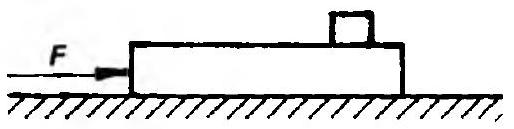
\includegraphics[width=0.4\linewidth]{images/2025_07_01_5b3ff9fa0d508c8e9f17g-048} Fig. 1.17\\

1.211. O cărămidă cu masa $m=5 \mathrm{~kg}$ se află pe un plan orizontal. Aceasta este deplasată uniform pe plan cu ajutorul unei cozi de lemn care face un unghi $\theta=30^{\circ}$ cu directia verticală (Fig. 1.18). Masa cozii este neglijabilă, iar coeficientul de frecare dintre cărămidă şi plan este $\mu=0,1$. Să se afle mărimea forței, orientată de-a lungul cozii, necesară pentru a face cărămida să alunece cu viteză constantă pe plan ($g=10 \mathrm{~m} / \mathrm{s}^{2}$).\\ A) $50 \mathrm{~N}$; B) $25 \mathrm{~N}$; C) $5,12 \mathrm{~N}$; D) $12,09 \mathrm{~N}$; E) $5 \mathrm{~N}$; F) $20,5 \mathrm{~N}$.\\ (Alexandru M. Preda)\\ \includegraphics[width=0.4\linewidth]{images/2025_07_01_5b3ff9fa0d508c8e9f17g-048(1) Fig. 1.18\\

1.212. O cărămidă cu masa $m=5 \mathrm{~kg}$ este aşezată pe un perete vertical şi apăsată cu o forță, $F$, de jos în sus, care face cu orizontala un unghi $\theta=45^{\circ}$. Dacă se consideră coeficientul de frecare $\mu=0,3$ şi $g=10 \mathrm{~m} / \mathrm{s}^{2}$ să se calculeze mărimea minimă a forței $F$ necesară pentru ca să nu cadă cărămida în jos.\\ A) $50 \mathrm{~N}$; B) $35 \mathrm{~N}$; C) $150,5 \mathrm{~N}$; D) $200,25 \mathrm{~N}$; E) $54,39 \mathrm{~N}$; F) $5,25 \mathrm{~N}$.\\ (Alexandru M. Preda)\\

1.213.* Presupunem că Pământul este perfect sferic şi are raza $R=6400 \mathrm{~km}$. Dacă considerăm $g=10 \mathrm{~m} / \mathrm{s}^{2}$ în toate punctele de pe Pământ, să se afle cu cât se micşorează greutatea unui om cu masa $m=100 \mathrm{~kg}$ când se deplasează de la pol la Ecuator.\\ A) $0 \mathrm{~N}$; B) $3,37 \mathrm{~N}$; C) $10,51 \mathrm{~N}$; D) $50 \mathrm{~N}$; E) $1,21 \mathrm{~N}$; F) $80,53 \mathrm{~N}$.\\ (Alexandru M. Preda)\\

1.214. Un corp se deplasează în sensul pozitiv al axei $Ox$ sub acțiunea unei forțe $F(x)=7 x+3$, unde $F$ se exprimă în Newtoni şi poziția $x$ în metri. Sub acțiunea acestei forţe corpul se deplasează între punctele $x_{1}=3 \mathrm{~m}$ şi $x_{2}=5 \mathrm{~m}$. Lucrul mecanic efectuat de această forță are valoarea:\\ A) $124 \mathrm{~J}$; B) $38 \mathrm{~J}$; C) $62 \mathrm{~J}$; D) $31 \mathrm{~J}$; E) $20 \mathrm{~J}$; F) $50 \mathrm{~J}$.\\ (Alexandru M. Preda)\\

1.215. Un avion având viteza de zbor (față de aerul înconjurător) de $234 \mathrm{~km} / \mathrm{h}$ trebuie să se deplaseze spre nord, în condițiile în care vântul bate spre est cu viteza de $25 \mathrm{~m} / \mathrm{s}$. Se cere viteza de deplasare a avionului faţă de pământ, precum şi unghiul pe care trebuie să îl facă direcția de zbor a fuzelajului avionului cu direcția nord.\\ A) $216 \mathrm{~km} / \mathrm{h}$, $\operatorname{arctg} \frac{5}{12}$ spre V-NV; B) $216 \mathrm{~km} / \mathrm{h}$, $\operatorname{arctg} \frac{5}{12}$ spre E-NE; C) $60 \mathrm{~m} / \mathrm{s}$, $\arcsin 0,416 \mathrm{spre} \mathrm{E}-\mathrm{NE}$; D) $65 \mathrm{~m} / \mathrm{s}$, $\arcsin 0,75 \mathrm{spre} \mathrm{V}-\mathrm{NV}$; E) $162,5 \mathrm{~km} / \mathrm{h}$, $\arcsin \frac{5}{13}$ spre V-NV; F) $180 \mathrm{~km} / \mathrm{h}, \arccos \frac{12}{13}$ spre E-NE.\\ (Corneliu Călin)\\

1.216. Un plan înclinat are rolul de a ridica greutați la înălțimea $h=4,4 \mathrm{~m}$, unghiul de înclinare fiind de $45^{\circ}$. De la baza acestui plan se lansează în sus pe plan cu viteza inițială $v_{0}=11 \mathrm{~m} / \mathrm{s}$ un corp ce se mişcă cu frecare, coeficientul de frecare dintre corp şi plan fiind $\mu=0,1$. Se cere timpul după care corpul ajunge la capătul superior al planului înclinat. Se consideră $g=10 \mathrm{~m} / \mathrm{s}^{2}$.\\ A) $0,78 \mathrm{~s}$; B) $2 \mathrm{~s}$; C) $1,41 \mathrm{~s}$; D) $1,73 \mathrm{~s}$; E) $0,707 \mathrm{~s}$; F) $0,577 \mathrm{~s}$.\\ (Corneliu Călin)\\

1.217.* Se consideră sistemul de corpuri reprezentat în Fig. 1.19. Corpul de masă $m_{1}$ se află situat la o distanță mai mare decât $h$ față de scripete. În momentul când $m_{2}$ atinge solul, viteza corpurilor va fi:\\ A) $v=\sqrt{2 g h}$; B) $v=\sqrt{\frac{2 m_{1} g h}{m_{1}+m_{2}}}$; C) $v=\sqrt{\frac{\left(m_{1}+m_{2}\right) g h}{m_{1}}}$; D) $v=\sqrt{\frac{m_{2}}{m_{1}} g h}$; E) $v=\sqrt{\frac{2 m_{2} g h}{m_{1}+m_{2}}}$; F) $v=\sqrt{g h}$.\\ (Gheorghe Stanciu)\\ 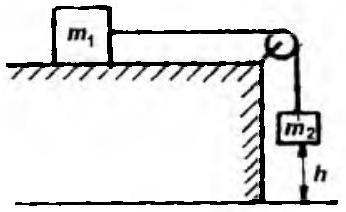
\includegraphics[width=0.4\linewidth]{images/2025_07_01_5b3ff9fa0d508c8e9f17g-050} Fig. 1.19\\

1.218. Sub acțiunea unui corp de masă $m^{\prime}$ un resort elastic suferă alungirea $\Delta l$. Suspendând resortul de tavanul unui mobil care suferă o mişcare pe un cerc de rază $R$, cu viteza $v$, să se arate dacă alungirea resortului este:\\ A) $\Delta l^{\prime}=\Delta l$; B) $\Delta l^{\prime}=\Delta l \sqrt{\frac{v^{2}}{R}+g}$; C) $\Delta l^{\prime}=\frac{\Delta l}{g} \sqrt{\frac{v^{4}}{R^{2}}+g^{2}}$; D) $\Delta l^{\prime}=\frac{\Delta l}{g} \sqrt{\frac{v^{2}}{R^{4}}+g^{2}}$; E) $\Delta l^{\prime}=\frac{\Delta l}{g} \sqrt{\frac{v^{2}}{R^{4}}-g^{2}}$; F) $\Delta l^{\prime}=\Delta l \sqrt{v^{2}-g^{2}}$.\\ (Gheorghe Stanciu)\\

1.219. Un corp prismatic de masă $M$ se poate deplasa pe o suprafață orizontală fără frecare. Pe suprafața acestuia se află un corp de masă $m$, coeficientul de frecare dintre corpuri fiind $\mu$. Dacă asupra corpului $M$ acționează o forță $F$, astfel încât corpul de masă $m$ începe să alunece, accelerația acestuia față de $M$ va fi:\\ A) $a=\mu \mathrm{mg}$; B) $a=\frac{\mu M g}{m}$; C) $a=\frac{\mu(M+m) g}{m}$; D) $a=\frac{F-\mu m g}{M}-\mu g$; E) $a=\frac{F-\mu M g}{m}-\mu g$; F) $a=\frac{F-\mu m g}{M+m}$.\\ (Gheorghe Stanciu)\\

1.220. Un plan înclinat sub unghiul $\alpha$, se poate deplasa fară frecare pe suprafața orizontală. Un corp de masă $m$ se află pe plan. Sub acțiunea unei forțe planul începe să se deplaseze accelerat, cu accelerația $\vec{a}$, în direcția opusă mişcării corpului pe plan. Cunoscând coeficientul de frecare $\mu$ să se arate dacă accelerația corpului faţă de suprafața planului înclinat este:\\ A) $g \sin \alpha$; B) $g \sin \alpha-a \cos \alpha$; C) $g \sin \alpha-\mu \cos \alpha$; D) $g \sin \alpha+a \cos \alpha-\mu(g \cos \alpha-a \sin \alpha)$; E) $g \sin \alpha-\mu(g \cos \alpha-a \sin \alpha)$; F) $\mu g \cos \alpha-(g \sin \alpha+a \cos \alpha)$.\\ (Gheorghe Stanciu)\\

1.221. Un vehicul de masã $m$ aflat sub acțiunea unei forțe de tracțiune $F$, se deplasează pe o suprafață orizonatlă cu un coeficient de frecare $\mu$, mărindu-şi viteza de la $0$ la $v$. Timpul după care atinge viteza $v$ este:\\ A) $t=\frac{m v^{2}}{F+\mu m g}$; B) $t=\frac{m v}{F-\mu m g}$; C) $t=\frac{F-\mu m g}{m v}$; D) $t=\frac{F+\mu m g}{v}$; E) $t=\frac{F}{v-\mu m g}$; F) $t=\frac{1}{2} \frac{m v}{F-\mu m g}$.\\ (Gheorghe Stanciu)\\

1.222. Un corp cade sub acțiunea propriei greutăți de la o înălțime $h$, necunoscută. Știind că în timpul $\tau$, înainte de a atinge solul, parcurge distanța $k h$, să se indice dacă timpul total al căderii este:\\ A) $l=5 \tau$; B) $t=\frac{\tau}{k}$; C) $t=k \tau$; D) $t=\tau \frac{1+\sqrt{1+k}}{k}$; E) $t=\tau \frac{1-\sqrt{1-k}}{k}$; F) $t=\tau \frac{1-\sqrt{1+k}}{k}$.\\ (Gheorghe Stanciu)\\

1.223. Asupra unui corp de masă $m=1 \mathrm{~kg}$, aşezat pe un plan orizontal, acționează forța $F$ având o direcţie care face un unghi $\alpha=\frac{\pi}{6} \mathrm{~rad}$ cu direcţia orizontală. Coeficientul de frecare dintre corp şi planul orizontal are valoarea $\mu=\frac{\sqrt{3}}{9}$ ($g=10 \mathrm{~m} / \mathrm{s}^{2}$). Valoarea maximă a forței $F$ pentru care corpul mai rămâne în repaus este:\\ A) $2 \mathrm{~N}$; B) $3 \mathrm{~N}$; C) $4 \mathrm{~N}$; D) $5 \mathrm{~N}$; E) $6 \mathrm{~N}$; F) $7 \mathrm{~N}$.\\ (Cone Gabriela)\\

1.224. Două bile sunt aruncate vertical în sus, din acelaşi punct, prima cu viteza $v_{01}=10 \mathrm{~m} / \mathrm{s}$, iar a doua după timpul $\tau=2 \mathrm{~s}$, cu viteza $v_{02}$. Bilele se întâlnesc:\\ A) la urcarea ambelor; B) la coborârea primeia şi urcarea celei de a doua; C) la coborârea ambelor; D) pe sol; E) nu se întâlnesc; F) nu se poate stabili din datele existente.\\ (Cone Gabriela)\\

1.225. Un tren cu masa $m=500 \mathrm{~t}$ se deplasează cu viteza constantă $v_{0}=72 \mathrm{~km} / \mathrm{h}$. La un moment dat trenul începe să frâneze şi parcurge până la oprire distanța $d=200 \mathrm{~m}$. Forța de frânare este egală cu:\\ A) $100 \mathrm{~kN}$; B) $200 \mathrm{~kN}$; C) $300 \mathrm{~kN}$; D) $4 \cdot 10^{5} \mathrm{~N}$; E) $5 \cdot 10^{5} \mathrm{~N}$; F) $5 \cdot 10^{4} \mathrm{~N}$.\\ (Cone Gabriela)\\

1.226. Un corp alunecă pe un plan înclinat cu unghiul $\alpha=45^{\circ}$ fațã de orizontală. Legea de mişcare a corpului este $s=b t^{2}$, unde $b=2,42$ în unități SI, iar $t$ este timpul. Coeficientul de frecare la alunecare pe planul înclinat are valoarea ($g=9,8 \mathrm{~m} / \mathrm{s}^{2}$):\\ A) $0,10$; B) $0,15$; C) $0,20$; D) $0,25$; E) $0,30$; F) $0,40$.\\ (Cone Gabriela)\\

1.227. De un fir trecut peste un scripete sunt legate două corpuri: unul, de masă $m_{1}=0,8 \mathrm{~kg}$, legat direct şi al doilea, de masă $m_{2}=0,2 \mathrm{~kg}$, legat prin intermediul unui resort de constantă elastică $k=50 \mathrm{~N} / \mathrm{m}$. Inițial firul fiind blocat, resortul se alungeşte după deblocare cu:\\ A) $4 \mathrm{~cm}$; B) $2,4 \mathrm{~cm}$; C) $1,2 \mathrm{~cm}$; D) $1 \mathrm{~cm}$; E) $0,2 \mathrm{~cm}$; F) $0,01 \mathrm{~cm}$.\\ (Cone Gabriela)\\

1.228. Pe o suprafaţă orizontală se află două corpuri de mase $m_{1}$ și $m_{2}$, legate printr-un resort. Coeficientul de frecare dintre corpuri şi planul orizontal este $\mu$. Forța minimă constantă orizontală care, acționând asupra primului corp, îl scoate din repaus pe al doilea este egală cu:\\ A) $m_{2} g$; B) $\mu\left(m_{1}+m_{2}\right) g$; C) $\mu m_{2} g$; D) $m_{2} g+\mu m_{1} g$; E) $m_{1} g$; F) $\mu \mathrm{m}_{1} g$.\\ (Cone Gabriela)\\

1.229. O locomotivă trage o garnitură de tren pe un plan orizontal, cu frecare, coeficientul de frecare fiind egal cu $\mu=0,015$. Accelerația trenului când viteza sa este egală cu jumătate din viteza maximă are valoarea:\\ A) $0,15 \mathrm{~m} / \mathrm{s}^{2}$; B) $1,5 \mathrm{~m} / \mathrm{s}^{2}$; C) $0,5 \mathrm{~m} / \mathrm{s}^{2}$; D) $0,1 \mathrm{~m} / \mathrm{s}^{2}$; E) $0,25 \mathrm{~m} / \mathrm{s}^{2}$; F) $1 \mathrm{~m} / \mathrm{s}^{2}$.\\ (Cone Gabriela)\\

1.230. Un corp cu masa $m=20 \mathrm{~kg}$, aflat la înălțimea $h=20 \mathrm{~m}$ deasupra solului, se sprijină de un resort orizontal comprimat cu $x=2 \mathrm{~cm}$. Resortul are constanta elastică $k=2000 \mathrm{~N} / \mathrm{m}$. Lăsând liber resortul, acesta împinge corpul, care parcurge pe orizontală, până la atingerea solului, distanța:\\ A) $1 \mathrm{~m}$; B) $0,4 \mathrm{~m}$; C) $10 \mathrm{~m}$; D) $12 \mathrm{~m}$; E) $13 \mathrm{~m}$; F) $15 \mathrm{~m}$.\\ (Cone Gabriela)\\

1.231. Alegeţi expresia care are unitatea de măsură a randamentului:\\ A) $\mathrm{J}$; B) $\mathrm{W}$; C) $\mathrm{Nm}$; D) $\mathrm{Js}$; E) $\frac{\mathrm{Ns}^{2}}{\mathrm{~kg} \mathrm{~m}}$; F) $\mathrm{m} / \mathrm{s}$.\\ (Cone Gabriela)\\

1.232. Impulsul:\\ A) este egal cu produsul dintre forţă şi viteză; B) este o mărime vectorială egală cu produsul dintre masă şi vectorul viteză; C) este egal cu raportul dintre lucrul mecanic şi timp; D) are expresia $\vec{p}=m \vec{a}$; E) este invers proporțional cu masa corpului; F) are sens opus vitezei.\\ (Cone Gabriela)\\

1.233. Un biciclist pleacă din punctul A spre B cu viteza de $18 \mathrm{~km} / \mathrm{h}$. În același moment, din B pleacă spre A un motociclist, cu viteza de $72 \mathrm{~km} / \mathrm{h}$, ajunge la punctul A apoi se întoarce, ajungând biciclistul la $72 \mathrm{~km}$ de A. Distanța dintre cele două puncte este:\\ A) $144 \mathrm{~km}$; B) $216 \mathrm{~km}$; C) $270 \mathrm{~km}$; D) $180 \mathrm{~km}$; E) $220 \mathrm{~km}$; F) $196 \mathrm{~km}$.\\ (Alexandru Lupaşcu)\\

1.234. O minge cade liber dintr-un turn şi atinge solul după $3 \mathrm{~s}$. Ştiind că $g=9,8 \mathrm{~m} / \mathrm{s}^{2}$ şi neglijând rezistența aerului, viteza medie a mingii în timpul căderii este:\\ A) $14,7 \mathrm{~m} / \mathrm{s}$; B) $9,8 \mathrm{~m} / \mathrm{s}$; C) $29,4 \mathrm{~m} / \mathrm{s}$; D) $19,6 \mathrm{~m} / \mathrm{s}$; E) $16,8 \mathrm{~m} / \mathrm{s}$; F) alt rezultat.\\ (Alexandru Lupaşcu)\\

1.235. Un vehicul care se deplasează cu $v_{1}=18 \mathrm{~km} / \mathrm{h}$ se opreşte pe o distanță de $3 \mathrm{~m}$. Considerând că acceleraţia de frânare rămâne aceeaşi, distanța de frânare la viteza $v_{2}=108 \mathrm{~km} / \mathrm{h}$ este egală cu:\\ A) $18 \mathrm{~m}$; B) $148 \mathrm{~m}$; C) $63 \mathrm{~m}$; D) $92 \mathrm{~m}$; E) $108 \mathrm{~m}$; F) $72 \mathrm{~m}$.\\ (Alexandru Lupaşcu)\\

1.236. O bilă este aruncată oblic în jos, cu unghiul $\alpha=30^{\circ}$ față de orizontală, dintr-un turn înalt de $60 \mathrm{~m}$. Viteza inițială a bilei este de $40 \mathrm{~m} / \mathrm{s}$. Se consideră $g=10 \mathrm{~m} / \mathrm{s}^{2}$. Viteza cu care bila atinge solul este de aproximativ:\\ A) $69,5 \mathrm{~m} / \mathrm{s}$; B) $43,6 \mathrm{~m} / \mathrm{s}$; C) $66,5 \mathrm{~m} / \mathrm{s}$; D) $58,3 \mathrm{~m} / \mathrm{s}$; E) $42,7 \mathrm{~m} / \mathrm{s}$; F) $52,9 \mathrm{~m} / \mathrm{s}$.\\ (Alexandru Lupaşcu)\\

1.237. Un corp cu masa de $25 \mathrm{~kg}$ este ținut timp de $1 \mathrm{~min}$ la înălțimea de $2 \mathrm{~m}$ deasupra solului. Ce lucru mecanic se efectuează în acest timp?\\ A) $3 \mathrm{~kJ}$; B) $50 \mathrm{~J}$; C) $50 \mathrm{~W}$; D) $300 \mathrm{~J}$; E) $0 \mathrm{~J}$; F) $0,83 \mathrm{~J}$.\\ (Alexandru Lupaşcu)\\

1.238. O rachetă care se deplasează cu viteza $v$, îşi porneşte motoarele şi ajunge la viteza $2 v$. În acest timp, prin consumarea carburantului, racheta pierde $50 \%$ din masa sa. Energia cinetică a rachetei:\\ A) scade de două ori; B) rămâne aceeaşi; C) creşte de două ori; D) creşte cu $50 \%$; E) creşte cu $75 \%$; F) creşte cu $150 \%$.\\ (Alexandru Lupaşcu)\\

1.239. Două bile de aceeaşi masă sunt aruncate cu aceeaşi viteză şi se ciocnesc cu un perete vertical. Prima bilă se ciocneşte perfect elastic, a doua rămâne lipită de perete. Care este răspunsul corect:\\ A) prima bilă cedează peretelui un impuls de două ori mai mare decât cea dea doua; B) a doua bilă cedează peretelui un impuls de două ori mai mare decât prima; C) ambele bile cedează peretelui acelaşi impuls; D) prima bilă cedează peretelui un impuls cu $50 \%$ mai mic decât a doua; E) prima bilă cedează peretelui un impuls cu $50 \%$ mai mare decât a doua; F) impulsurile cedate peretelui de cele două bile nu se pot compara.\\ (Alexandru Lupaşcu)\\

1.240.* Un punct material execută o mişcare circulară uniformă, caracterizată de $\vec{\omega}=const.$, care este analizată dintr-un sistem de referință inerțial. Una dintre afirmațiile următoare este falsă:\\ A) forța centrifugă este reacțiunea la forța centripetă şi reciproc; B) pentru analiza mişcării nu este nevoie să considerăm forța centrifugă de inerție; C) punctul material execută mişcarea circulară uniformă sub acțiunea forței centripete; D) asupra punctului material acționează simultan forța centrifugă şi forța centripetă; E) forța centrifugă este proporțională cu raza de girație; F) forța centripetă nu modifică energia cinetică a punctului material.\\ (Eugen Scarlat)\\

1.241.* Un corp execută o mişcare circulară uniformă, caracterizată de $\vec{\omega}=const.$, care este analizată dintr-un sistem de referință inerțial. Una dintre afirmațiile următoare este falsă:\\ A) forța centrifugă este creată de corp şi suportată de mediu; B) corpul execută mişcarea circulară uniformă sub acțiunea forței centripete; C) corpul execută mişcarea circulară uniformă sub acțiunea forței centrifuge; D) forța centripetă este creată de mediu şi suportată de corp; E) forța centripetă este proporțională cu raza de girație; F) forța centrifugă este proporțională cu viteza tangențială a corpului.\\ (Eugen Scarlat)\\

1.242.* Un punct material execută o mişcare circulară uniformă. Analizăm mişcarea dintr-un sistem de referință fixat de corp. Una dintre afirmațiile următoare este falsă:\\ A) forța centrifugă de inerție şi forța centripetă acționează asupra punctului material şi se echilibrează reciproc; B) forța centrifugă de inerție este o pseudoforță; C) modulul forței centrifuge de inerție este proporțional cu masa punctului material; D) asupra punctului material acționează simultan forța centrifugă şi forța centripetă; E) modulul forţei centrifuge, modulul forței centripete şi modulul forței centrifuge de inerție sunt egale între ele; F) punctul material este în repaus.\\ (Eugen Scarlat)\\

1.243.* Un punct material execută o mişcare circulară uniformă. Analizăm mişcarea dintr-un sistem de referință fixat de corp. Una singură dintre afirmațiile următoare este adevărată:\\ A) forța centrifugă de inerție şi forța centripetă acționează asupra punctului material şi se echilibrează reciproc; B) forța centrifugă de inerție şi forța centrifugă acționează asupra punctului material şi se echilibrează reciproc; C) forța centrifugă şi forța centripetă acționează asupra punctului material şi se echilibrează reciproc; D) forţa centrifugă este reacțiunea la forța centrifugă de inerție și reciproc; E) forța centripetă este reacțiunea la forța centrifugă de inerție și reciproc; F) forța centrifugă este o pseudoforță.\\ (Eugen Scarlat)\\

1.244.* Un corp loveşte frontal un perete. În ce raport este forța medie de contact, în cazul ciocnirii elastice, față de forța în cazul ciocnirii plastice, dacă timpul de ciocnire este acelaşi?\\ A) $1: 1$; B) $2: 1$; C) $1: 2$; D) $2: 3$; E) $3: 2$; F) $\sqrt{2}: 1$.\\ (Eugen Scarlat)\\

1.245. Un om, a cărui masă este $m$, parcurge uniform lungimea unei bărci $l$ (de la proră la pupă), în timpul $\tau$. În acest timp, barca, a cărei masă este $M$, se deplasează faṭă de apă pe o distanță $d$. Cum se modifică această distanță dacă timpul $\tau$ se dublează?\\ A) creşte de 2 ori; B) creşte de $\sqrt{2}$ ori; C) creşte de $2 \sqrt{2}$ ori; D) nu se modifică; E) scade de 2 ori; F) scade de $\sqrt{2}$ ori.\\ (Eugen Scarlat)\\

1.246.* Două bile identice se mişcă una spre cealaltă cu viteze egale în modul. La ciocnirea lor, perfect plastică, se degajă o cantitate de căldură $Q$. Cum se modifică căldura degajată, dacă viteza uneia dintre bile se triplează?\\ A) creşte de $\sqrt{3}$ ori; B) creşte de 3 ori; C) creşte de 4 ori; D) creşte de 9 ori; E) creşte de $3 \sqrt{3}$ ori; F) nu se modifică.\\ (Eugen Scarlat)\\

1.247. Un resort vertical este comprimat puternic şi apoi lăsat să se destindă brusc, aruncând în sus un mic corp până la înălțimea $h$. Dacă se neglijează frecările cu aerul și dimensiunile resortului, precizați la ce înălțime va fi aruncat micul corp, dacă resortul este comprimat la jumătate față de situația anterioară.\\ A) $h \frac{1}{2}$; B) $h \frac{1}{4}$; C) $h$; D) $h \frac{1}{3}$; E) $h \frac{\sqrt{2}}{2}$; F) $h \frac{\sqrt{2}}{4}$.\\ (Eugen Scarlat)\\

1.248.* Două bile de mase egale sunt suspendate pe fire paralele, astfel încât bilele se ating. Prima bilă este deviată până la o înălțime $h$ și lăsată liber. La ce inălțime se ridică prima bilă după ciocnirea perfect elastică cu bila a doua?\\ A) $h \frac{\sqrt{3}}{2}$; B) $h \frac{1}{2}$; C) $h$; D) $2 h$; E) $h \frac{\sqrt{2}}{3}$; F) zero.\\ (Eugen Scarlat)\\

1.249.* O particulă stă inițial în punctul A pe o sferă de rază $R$, conform Fig. 1.20. Particula începe să alunece pe sferă, fără frecare. La ce unghi se desprinde particula?\\ A) $\cos \theta=\frac{\sqrt{3}}{2}$; B) $\cos \theta=\frac{2}{\sqrt{3}}$; C) $\cos \theta=\frac{2}{3}$; D) $\operatorname{tg} \theta=\frac{1}{2}$; E) $\sin \theta=\frac{2}{3}$; F) $\operatorname{tg} \theta=\frac{2}{3}$.\\ (Alexandrina Nenciu)\\ 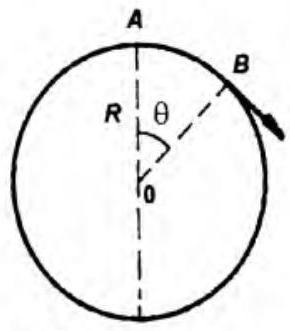
\includegraphics[width=0.4\linewidth]{images/2025_07_01_5b3ff9fa0d508c8e9f17g-057(1)} Fig. 1.20\\

1.250.* O particulă de masă $m$ alunecă fără frecare pornind din $A$ pe o sferă de rază $R$ şi se desprinde de sferă atunci când $\cos \theta=\frac{2}{3}$ (conform Fig. 1.21). În ce punct atinge Pámântul?\\ A) $\mathrm{A}^{\prime} \mathrm{M}=\frac{13 \sqrt{5}}{27} R$; B) $\mathrm{A}^{\prime} \mathrm{M}=2 R$; C) $\mathrm{A}^{\prime} \mathrm{M}=\frac{5 R}{3}$; D) $\mathrm{A}^{\prime} \mathrm{M}=\frac{10}{3} \sqrt{\frac{R}{3}}$; E) $\mathrm{A}^{\prime} \mathrm{M}=\frac{13 \sqrt{5} R}{9}$; F) $\mathrm{A}^{\prime} \mathrm{M}=\frac{13 \sqrt{5} R}{3}$.\\ (Alexandrina Nenciu)\\ 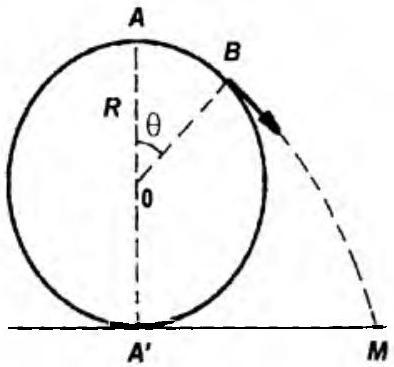
\includegraphics[width=0.4\linewidth]{images/2025_07_01_5b3ff9fa0d508c8e9f17g-057} Fig. 1.21\\

1.251.* O bandă circulară de masă $m$ şi rază $r$ se rotește în jurul unei axe verticale care trece prin centru, perpendiculară pe planul benzii, astfel încât fiecare punct:are viteza $v$. Calculați tensiunea din bandă, presupunând că aceasta este inextensibilă.\\ A) $T=\frac{m v^{2}}{\pi r^{2}}$; B) $T=\frac{m v^{2}}{2 \pi r}$; C) $T=\frac{m v^{2}}{r}$; D) $T=\frac{m v^{2}}{2 r}$; E) $T=\frac{m v^{2}}{2}$; F) $T=\frac{m v}{r}$.\\ (Alexandrina Nenciu)\\

1.252.* Într-un parc de distracții maşinile se deplaseazã pe o buclă verticală, conform Fig. 1.22. Dacă în partea superioară bucla este un cerc de rază $R=10 \mathrm{~m}$, iar punctul cel mai înalt se află la înălțimea $h=30 \mathrm{~m}$ de sol, care este viteza minimă cu care trebuie să intre maşina în buclă, pentru a nu cădea.\\ A) $50 \mathrm{~m} / \mathrm{s}$; B) $23 \mathrm{~m} / \mathrm{s}$; C) $10 \mathrm{~m} / \mathrm{s}$; D) $26,1 \mathrm{~m} / \mathrm{s}$; E) $\mathrm{s}=-\mathrm{s}$; F) $100 \mathrm{~m} / \mathrm{s}$.\\ (Alexandrina Nenciu)\\ 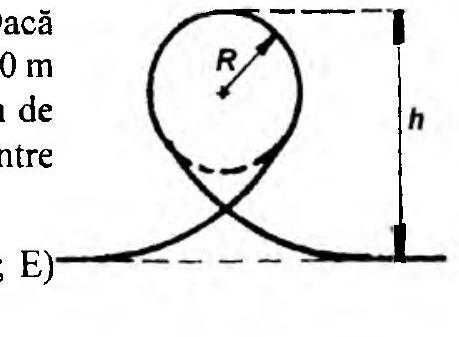
\includegraphics[width=0.4\linewidth]{images/2025_07_01_5b3ff9fa0d508c8e9f17g-057(2)} Fig. 1.22\\

1.253.* Într-un parc de distracții, maşinile alunecă de la înălțimea $h=50 \mathrm{~m}$, pe o curbă ca în Fig. 1.23. Dacă pasagerii suportă o accelerație egală cu $8 g$, care trebuie să fie raza $R$ a cercului de la baza curbei?\\ A) $50 \mathrm{~m}$; B) $3 \mathrm{~m}$; C) $7,2 \mathrm{~m}$; D) $14,3 \mathrm{~m}$; E) $50,2 \mathrm{~m}$; F) $17,2 \mathrm{~m}$.\\ (Alexandrina Nenciu)\\ 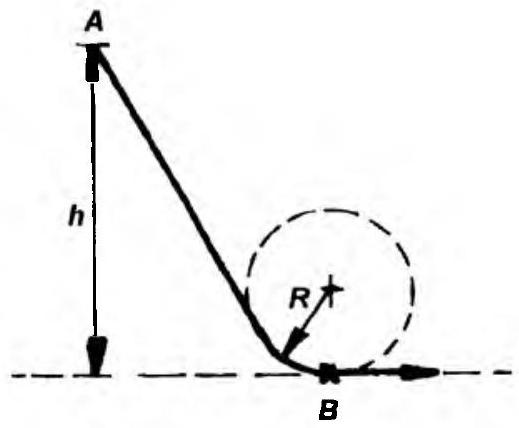
\includegraphics[width=0.4\linewidth]{images/2025_07_01_5b3ff9fa0d508c8e9f17g-058(1)} Fig. 1.23\\

1.254.* Una din metodele de măsurare a vitezei proiectilelor constă în folosirea unui pendul balistic. Acesta este un corp de lemn de masă $m_{2}$, suspendat cu ajutorul a două fire lungi (Fig. 1.24). Inițial pendulul este în repaus. Un proiectil de masă $m_{1}$ loveşte orizontal corpul din lemn și rămâne încastrat, făcând ca pendulul şi proiectilul sã se ridice la înălțimea $h$. Dacă masa pendulului este $m_{2}=4 \mathrm{~kg}$, masa proiectilului este $m_{1}=9,7 \mathrm{~g}$ şi în urma impactului se ridică la $h=19 \mathrm{~cm}$, care este viteza inițială a proiectilului? ($g=9,8 \mathrm{~m} / \mathrm{s}^{2}$).\\ A) $10 \mathrm{~m} / \mathrm{s}$; B) $256 \mathrm{~m} / \mathrm{s}$; C) $1452 \mathrm{~m} / \mathrm{s}$; D) $3452 \mathrm{~m} / \mathrm{s}$; E) $960 \mathrm{~m} / \mathrm{s}$; F) $798 \mathrm{~m} / \mathrm{s}$.\\ (Alexandrina Nenciu)\\ 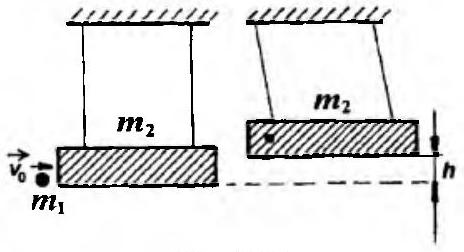
\includegraphics[width=0.4\linewidth]{images/2025_07_01_5b3ff9fa0d508c8e9f17g-058} Fig. 1.24\\

1.255.* O piatră aruncată pe orizontală cu viteza $v_{0}=15 \mathrm{~m} / \mathrm{s}$ de pe acoperişul unei case, cade pe sol sub unghiul $\alpha=60^{\circ}$ față de orizontală. Care este înălțimea $h$ a casei? ($g=9,8 \mathrm{~m} / \mathrm{s}^{2}$).\\ A) $30,3 \mathrm{~m}$; B) $34,4 \mathrm{~m}$; C) $36,1 \mathrm{~m}$; D) $39,2 \mathrm{~m}$; E) $35 \mathrm{~m}$; F) $28 \mathrm{~m}$.\\ (George Ionescu)\\

1.256.* Un automobil trece peste un pod convex cu viteza $v=72 \mathrm{~km} / \mathrm{h}$. Să se calculeze raza de curbură a podului la mijlocul acestuia, știind ca în acest punct automobilul apasă cu o forță egală cu $4 / 5$ din greutatea sa. Se va aproxima $g=10 \mathrm{~m} / \mathrm{s}^{2}$.\\ A) $180 \mathrm{~m}$; B) $200 \mathrm{~m}$; C) $240 \mathrm{~m}$; D) $270 \mathrm{~m}$; E) $320 \mathrm{~m}$; F) $254 \mathrm{~m}$.\\ (George Ionescu)\\

1.257.* De pe vârful unei sfere de rază $R=3 \mathrm{~m}$ alunecă liber în jos, fără viteză inițială, un mic corp. La ce înălțime de vârful sferei se va desprinde corpul?\\ A) $0,5 \mathrm{~m}$; B) $0,7 \mathrm{~m}$; C) $1 \mathrm{~m}$; D) $1,2 \mathrm{~m}$; E) $1,3 \mathrm{~m}$; F) $1,5 \mathrm{~m}$.\\ (George Ionescu)\\

1.258. Un om deplasează uniform, pe un drum drept şi orizontal, o sanie cu masa de $50 \mathrm{~kg}$, trăgând-o cu o forță constantă de $300 \mathrm{~N}$ prin intermediul unui fir înclinat cu $30^{\circ}$ faţă de orizontală. Calculați valoarea coeficientului de frecare. ($g=9,8 \mathrm{~m} / \mathrm{s}^{2}$).\\ A) $0,55$; B) $0,63$; C) $0,91$; D) $0,76$; E) $0,85$; F) $0,38$.\\ (George Ionescu)\\

1.259. Cu câți $\mathrm{kW}$ lucrează o locomotivă care dezvoltă o forță de tracțiune de $30000 \mathrm{~N}$ şi remorchează un tren ce se deplasează cu $54 \mathrm{~km} / \mathrm{h}$?\\ A) $260 \mathrm{~kW}$; B) $300 \mathrm{~kW}$; C) $370 \mathrm{~kW}$; D) $450 \mathrm{~kW}$; E) $560 \mathrm{~kW}$; F) $415 \mathrm{~kW}$.\\ (George Ionescu)\\

1.260. Pentru ca un automobil să se deplaseze cu viteza de $30 \mathrm{~m} / \mathrm{s}$, motorul dezvoltă o putere de $6 \cdot 10^{4} \mathrm{~W}$. Ce distanță poate parcurge automobilul cu $1 \mathrm{~l}$ de benzină, ştiind că energia furnizată de acesta motorului este de $8 \cdot 10^{6} \mathrm{~J} / \mathrm{l}$.\\ A) $3 \mathrm{~km}$; B) $3,5 \mathrm{~km}$; C) $4 \mathrm{~km}$; D) $4,5 \mathrm{~km}$; E) $6 \mathrm{~km}$; F) $7,2 \mathrm{~km}$.\\ (George Ionescu)\\

1.261. Pentru a atinge viteza de regim pornind din repaus pe un drum orizontal, un camion este supus un timp $t=10 \mathrm{~s}$ acțiunii unei forțe de tracțiune $F=6 \mathrm{~kN}$, care efectuează în acest interval un lucru mecanic $L=600 \mathrm{~kJ}$. Să calculeze accelerația imprimată camionului.\\ A) $1 \mathrm{~m} / \mathrm{s}^{2}$; B) $2 \mathrm{~m} / \mathrm{s}^{2}$; C) $3 \mathrm{~m} / \mathrm{s}^{2}$; D) $4 \mathrm{~m} / \mathrm{s}^{2}$; E) $5 \mathrm{~m} / \mathrm{s}^{2}$; F) $2,5 \mathrm{~m} / \mathrm{s}^{2}$.\\ (George Ionescu)\\

1.262. Cu ce forţă minimă orizontală trebuie să acționăm asupra unui corp de masă $m=1 \mathrm{~kg}$, ce se află pe un plan înclinat de unghi $\alpha=30^{\circ}$, pentru ca corpul să rămână în repaus? Se dau $\mu=0,2$, $g=10 \mathrm{~m} / \mathrm{s}^{2}$.\\ A) $5,02 \mathrm{~N}$; B) $11 \mathrm{~N}$; C) $3,77 \mathrm{~N}$; D) $1,78 \mathrm{~N}$; E) $4,03 \mathrm{~N}$; F) $2,15 \mathrm{~N}$.\\ (George Ionescu)\\

1.263.* O bilă de masă $m=2 \mathrm{~kg}$ este suspendată de un fir de lungime $l=0,4 \mathrm{~m}$. Se imprimă bilei o mişcare de rotație uniformă în planul orizontal (pendul conic) cu viteza unghiulară $\omega=7 \mathrm{rad} / \mathrm{s}$. Să se calculeze energia cinetică a bilei.\\ A) $7,3 \mathrm{~J}$; B) $5,8 \mathrm{~J}$; C) $9,5 \mathrm{~J}$; D) $4,7 \mathrm{~J}$; E) $9,8 \mathrm{~J}$; F) $8,3 \mathrm{~J}$.\\ (George Ionescu)\\

1.264.* Un obiect, aruncat sub unghiul $\alpha=30^{\circ}$ fațā de orizontală se află la aceeaşi înălțime $h$ la două momente diferite $t_{1}=3 \mathrm{~s}$ şi $t_{2}=5 \mathrm{~s}$ de la începutul mişcării. Să se determine viteza $v_{0}$ și înălțimea $h$. Se dă $g=10 \mathrm{~m} / \mathrm{s}^{2}$.\\ A) $70 \mathrm{~m} / \mathrm{s}$ şi $68 \mathrm{~m}$; B) $80 \mathrm{~m} / \mathrm{s}$ şi $75 \mathrm{~m}$; C) $90 \mathrm{~m} / \mathrm{s}$ şi $82 \mathrm{~m}$; D) $78 \mathrm{~m} / \mathrm{s}$ şi $102 \mathrm{~m}$; E) $45 \mathrm{~m} / \mathrm{s}$ şi $80 \mathrm{~m}$; F) $73 \mathrm{~m} / \mathrm{s}$ şi $90 \mathrm{~m}$.\\ (George Ionescu)\\

1.265. Un pendul format dintr-un fir de lungime $l=1,6 \mathrm{~m}$ și o bilă de masă $m=0,5 \mathrm{~kg}$ aflat în poziție de repaus, primeşte un impuls $p=2 \mathrm{~N} \cdot \mathrm{~s}$. Să se calculeze unghiul maxim pe care îl face firul cu poziția de echilibru.\\ A) $30^{\circ}$; B) $45^{\circ}$; C) $60^{\circ}$; D) $75^{\circ}$; E) $90^{\circ}$; F) $180^{\circ}$.\\ (George Ionescu)\\

1.266. Ce viteză inițială i se imprimă unui obuz lansat sub unghiul $\alpha=30^{\circ}$ pentru a cădea la distanța $d=17300 \mathrm{~m}$? Se aproximează $g=10 \mathrm{~m} / \mathrm{s}^{2}$. Se neglijează rezistența aerului.\\ A) $446 \mathrm{~m} / \mathrm{s}$; B) $495 \mathrm{~m} / \mathrm{s}$; C) $502,1 \mathrm{~m} / \mathrm{s}$; D) $385 \mathrm{~m} / \mathrm{s}$; E) $324 \mathrm{~m} / \mathrm{s}$; F) $523 \mathrm{~m} / \mathrm{s}$.\\ (George Ionescu)\\

1.267.* De un lanţ rigid, ce rezistă la o tensiune maximă $T_{\max}=40 \mathrm{~N}$, este suspendat un corp cu masa $m=1 \mathrm{~kg}$. Care este unghiul pe care îl poate face lanţul cu poziția de echilibru, astfel ca lanțul să nu se rupă în timpul oscilației?\\ A) $75^{\circ}$; B) $90^{\circ}$; C) $110^{\circ}$; D) $120^{\circ}$; E) $60^{\circ}$; F) $45^{\circ}$.\\ (George Ionescu)\\

1.268. Pe un plan înclinat de unghi $\alpha=30^{\circ}$ se află un corp de masă $m=50 \mathrm{~kg}$, asupra căruia acționează o forță orizontală $F=294 \mathrm{~N}$ (Fig. 1.25). Neglijând frecările, să se calculeze accelerația cu care se mişcă corpul şi forța cu care apasă asupra planului. ($g=10 \mathrm{~m} / \mathrm{s}^{2}$)\\ A) $12,1 \mathrm{~m} / \mathrm{s}^{2}$ şi $360,3 \mathrm{~N}$; B) $9 \mathrm{~m} / \mathrm{s}^{2}$ şi $382,5 \mathrm{~N}$; C) $10,1 \mathrm{~m} / \mathrm{s}^{2}$ şi $285,5 \mathrm{~N}$; D) $8 \mathrm{~m} / \mathrm{s}^{2}$ şi $422 \mathrm{~N}$; E) $7,5 \mathrm{~m} / \mathrm{s}^{2}$ şi $324 \mathrm{~N}$; F) $8,7 \mathrm{~m} / \mathrm{s}^{2}$ şi $385 \mathrm{~N}$.\\ (George Ionescu)\\ 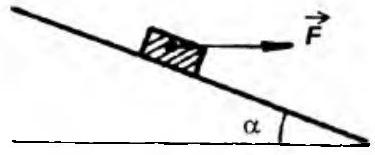
\includegraphics[width=0.4\linewidth]{images/2025_07_01_5b3ff9fa0d508c8e9f17g-061(1)} Fig. 1.25\\

1.269. De pe un acoperiş cad, una după alta, două picături de apă (Fig. 1.26). După un timp $\tau=2 \mathrm{~s}$ de la începutul căderii celei de-a doua picături, distanța dintre ele este $\Delta h=25 \mathrm{~m}$. Cu cât timp înaintea desprinderii celei de-a doua picături s-a desprins prima picătură de pe acoperiş?\\ A) $3 \mathrm{~s}$; B) $7 \mathrm{~s}$; C) $1 \mathrm{~s}$; D) $0,7 \mathrm{~s}$; E) $1,8 \mathrm{~s}$; F) $2,4 \mathrm{~s}$.\\ (George Ionescu)\\ 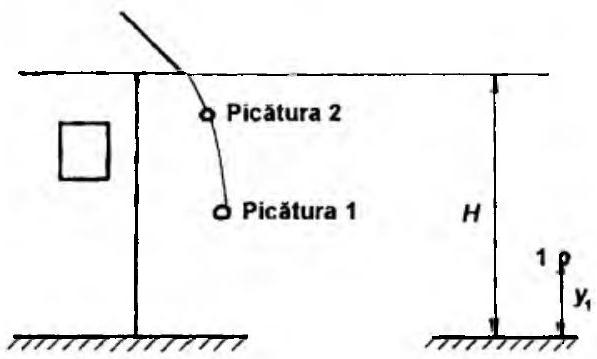
\includegraphics[width=0.4\linewidth]{images/2025_07_01_5b3ff9fa0d508c8e9f17g-061(2)} Fig. 1.26\\

1.270. Un teleschi funcționeazǎ pe o pantă de $240 \mathrm{~m}$, înclinatǎ la $30^{\circ}$. Cablul se deplasează cu $10 \mathrm{~km} / \mathrm{h}$ şi trage simultan 100 schiori, cu o masă medie de $72 \mathrm{~kg}$. Estimați puterea necesară pentru funcționarea teleschiului. (Se neglijează frecarea, considerăm $g=9,8 \mathrm{~m} / \mathrm{s}^{2}$).\\ A) $1000 \mathrm{~J} / \mathrm{s}$; B) $49000 \mathrm{~W}$; C) $100 \mathrm{~kW}$; D) $0,1 \mathrm{~GW}$; E) $50 \mathrm{~kJ} / \mathrm{h}$; F) $98 \mathrm{~kW}$.\\ (Ionuț Puică)\\

1.271. Ce accelerație trebuie să aibă căruciorul din Fig. 1.27 astfel încât corpul A să nu cadă? Coeficientul de frecare dintre corp şi cărucior este $\mu$.\\ A) mai mare sau egală cu $g / \mu$; B) $g$; C) $\mu g$; D) infinită; E) problema nu are soluție; F) $g / \mu$.\\ (Ionuț Puică)\\ 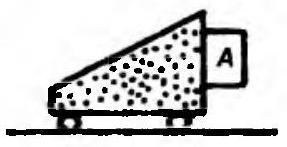
\includegraphics[width=0.4\linewidth]{images/2025_07_01_5b3ff9fa0d508c8e9f17g-061} Fig. 1.27\\

1.272.* Un vagon descoperit de cale ferată cu masa de $10 \mathrm{~t}$ alunecă fără frecare de-a lungul unor şine orizontale. Plouă puternic, ploaia căzând vertical. Vagonul este inițial gol şi se mişcă cu o viteză de $1 \mathrm{~m} / \mathrm{s}$. Care este viteza vagonului după ce s-a deplasat suficient pentru a strânge $1000 \mathrm{~kg}$ de apă de ploaie?\\ A) $0,91 \mathrm{~m} / \mathrm{s}$; B) $0,5 \mathrm{~m} / \mathrm{s}$; C) zero; D) $10 \mathrm{~cm} / \mathrm{s}$; E) $8 \mathrm{dm} / \mathrm{s}$; F) $10 \mathrm{~km} / \mathrm{h}$.\\ (Ionuț Puică)\\

1.273. Un ascensor şi încărcătura lui au o masă totală de $800 \mathrm{~kg}$. Să se determine tensiunea $T$ din cablul de susținere atunci când ascensorul, care se mişcă inițial în jos cu $10 \mathrm{~m} / \mathrm{s}$, este oprit cu accelerație constantă pe o distanță de $25 \mathrm{~m}$. ($g=9,8 \mathrm{~m} / \mathrm{s}^{2}$).\\ A) $9440 \mathrm{~N}$; B) $7840 \mathrm{~N}$; C) $1600 \mathrm{~N}$; D) egală cu greutatea ascensorului; E) nu se poate calcula din datele problemei; F) $6240 \mathrm{~N}$.\\ (Ionuț Puică)\\

1.274. Motorul unei bărci furnizează elicei o putere de $30 \mathrm{~kW}$ atunci când barca se deplasează cu o viteză de $30 \mathrm{~km} / \mathrm{h}$. Care ar fỉ tensiunea din cablu, dacă barca ar fi remorcată cu aceeaşi viteză?\\ A) $1000 \mathrm{~N}$; B) $49 \mathrm{~kN}$; C) $3600 \mathrm{~N}$; D) $0,1 \mathrm{~GN}$; E) $50 \mathrm{~kN}$; F) $98 \mathrm{~N}$.\\ (Ionuț Puică)\\

1.275.* O minge de greutate $G$ este legată de o coardã şi pusă în mişcare de rotație pe un cerc vertical. Tensiunea din coardă în punctul cel mai de jos este mai mare decât cea din punctul cel mai înalt cu o valoare egală cu:\\ A) depinde de viteza de rotație; B) tensiunile sunt egale; C) $G$; D) $6 G$; E) $2 G$; F) depinde de lungimea corzii.\\ (Ionuț Puică))\\

1.276. Două trenuri aflate în mişcări rectilinii paralele uniform accelerate, în același sens, se reîntâlnesc după $14 \mathrm{~s}$ de la depășire. După cât timp de la prima depăşire trenurile vor avea aceeaşi viteză instantanee?\\ A) $20 \mathrm{~s}$; B) $10 \mathrm{~s}$; C) $1 \mathrm{~min}$; D) $5 \mathrm{~s}$; E) $7 \mathrm{~s}$; F) $9,8 \mathrm{~s}$.\\ (Radu Chişleag)\\

1.277. Un cart, cu masa totală de $100 \mathrm{~kg}$, parcurge uniform o rampă lungă de $3,6 \mathrm{~km}$, în $4 \mathrm{~min}$ şi $5 \mathrm{~s}$. La fiecare tură de roată cu o lungime de $180 \mathrm{~cm}$, centrul său de masă urcă cu $5 \mathrm{~cm}$. Care este puterea consumată de cart neglijând rezistența aerului şi frecarea cu solul? Se cunoaşte: $g=9,8$ u.S.I.\\ A) $0,8 \mathrm{~kWh}$; B) $400 \mathrm{~J}$; C) $400 \mathrm{~W}$; D) $500 \mathrm{~Wh}$; E) $0,4 \mathrm{~kWh}$; F) $500 \mathrm{~J}$.\\ (Radu Chişleag)\\

1.278. Un om având înălțimea $h=180 \mathrm{~cm}$ se deplasează cu viteza $v=2 \mathrm{~ms}^{-1}$, trecând pe sub un felinar situat la înălțimea de $5,4 \mathrm{~m}$. Cu ce viteză $V$ se alungeşte umbra omului pe sol?\\ A) $2 \mathrm{~ms}^{-1}$; B) $6 \mathrm{~ms}^{-1}$; C) $4 \mathrm{~m} / \mathrm{s}$; D) $5,4 \mathrm{~km} / \mathrm{h}$; E) $7,5 \mathrm{~m} / \mathrm{s}$; F) $3 \mathrm{~m} / \mathrm{s}$.\\ (Radu Chişleag)\\

1.279. Un leu cu greutatea de $980 \mathrm{~N}$ se mişcă accelerat, din repaus până la viteza de $36 \mathrm{~km} / \mathrm{h}$, în $1,25 \mathrm{~s}$. Care a fost puterea medie necesară pentru această accelerare, neglijând frecările?\\ A) $10 \mathrm{~kW}$; B) $5 \mathrm{~kW}$; C) $2 \mathrm{~kW}$; D) $50 \mathrm{~kJ}$; E) $4 \mathrm{~kW}$; F) $4 \mathrm{~kJ}$.\\ (Radu Chişleag)\\

1.280. O şopârlă se află într-un colț de jos al unei cutii cubice transparente cu latura de $200 \mathrm{~cm}$ şi își vede puiul agățat în colțul opus de sus al cutiei. Care este cel mai scurt timp în care puiul nemişcat poate primi ajutorul mamei, dacă mama se poate deplasa pe suprafața cutiei în orice direcție cu viteza de $10 \mathrm{~cm} / \mathrm{s}$?\\ A) nu se poate rezolva cu datele din problemă; B) $2 \mathrm{~min}$ şi $3 \mathrm{~s}$; C) $447 \mathrm{~s}$; D) $89,4 \mathrm{~s}$; E) $67 \mathrm{~s}$; F) $2 \mathrm{~min}$ şi $3 / 4 \mathrm{~s}$.\\ (Radu Chişleag)\\

1.281. Doi prieteni $El$ şi $Ea$ se află la distanța de $100 \mathrm{~m}$ unul de altul, pe o direcție paralelă cu un zid. Apelul $Lui$ este auzit de $Ea$ de 2 ori la un interval de $t=100 \mathrm{cs}$. Să se determine distanța dintre prieteni şi zid, dacă viteza sunetului în aer este de $340 \mathrm{~m} / \mathrm{s}$.\\ A) $270 \mathrm{~m}$; B) $185 \mathrm{~m}$; C) $214 \mathrm{~m}$; D) $60 \mathrm{~m}$; E) $107 \mathrm{~m}$; F) $120 \mathrm{~m}$.\\ (Radu Chişleag)\\

1.282. Ce forță medie este necesară pentru a frâna un cărucior în $5 \mathrm{~s}$, dacă impulsul acestuia, înaintea frânării, este de $100 \mathrm{~kg} \cdot \mathrm{~m} \cdot \mathrm{~s}^{-1}$?\\ A) $5 \mathrm{~m} / \mathrm{s}$; B) $20 \mathrm{~N}$; C) $100 \mathrm{~kg} \cdot \mathrm{~m} \cdot \mathrm{~s}^{-1}$; D) $5 \mathrm{~kN}$; E) $40 \mathrm{~kN}$; F) $20 \mathrm{~kN}$.\\ (Radu Chişleag)\\

1.283. Un tren parcurge prima jumătate a distanței Bucureşti-Alexandria cu viteza $v_{1}$, iar restul traseului cu viteza $v_{2}=21,6 \mathrm{~km} / \mathrm{h}$. Dacă viteza medie pe toată distanța a fost $v_{m}=10 \mathrm{~ms}^{-1}$, care este $v_{1}$?\\ A) $21,6 \mathrm{~km} / \mathrm{h}$; B) $30 \mathrm{~m} / \mathrm{s}$; C) $54 \mathrm{~km} / \mathrm{h}$; D) $36 \mathrm{~m} / \mathrm{s}$; E) $20 \mathrm{~m} / \mathrm{s}$; F) $14 \mathrm{~m} / \mathrm{s}$.\\ (Radu Chişleag)\\

1.284.* Care trebuie să fie raza minimă a pistei circulare a unui velodrom improvizat plan pe care se deplasează cicliştii, cu $54 \mathrm{~km} / \mathrm{h}$, dacă coeficientul de frecare la alunecare laterală al roților bicicliştilor este $\mu=0,5$? ($g=9,8 \mathrm{~m} / \mathrm{s}^{2}$).\\ A) $60 \mathrm{~m}$; B) $408 \mathrm{~dm}$; C) $54 \mathrm{~m}$; D) $508 \mathrm{~dm}$; E) $459 \mathrm{~dm}$; F) $64 \mathrm{~m}$.\\ (Radu Chişleag)\\

1.285. Un elicopter parcurge într-o regiune cu vânt constant de direcția $AB$, la înălțimea de zbor de $1 \mathrm{~km}$, traseul $AB$ în $50 \mathrm{~min}$ şi traseul invers, $BA$, în $70 \mathrm{~min}$. În cât timp ar parcurge traseul $BA$, un balon care ar pluti la aceeaşi înălțime cu avionul?\\ A) $60 \mathrm{~min}$; B) $120 \mathrm{~min}$; C) balonul nu poate parcurge traseul $BA$; D) $24 \mathrm{~h}$; E) $350 \mathrm{~h}$; F) $3 \mathrm{~zile}$.\\ (Radu Chişleag)\\

1.286. Un tren cu masa $M=440 \mathrm{~t}$ se deplasează uniform şi rectiliniu, cu viteza $v=36 \mathrm{~km} / \mathrm{h}$, având coeficientul de frecare $\mu=0,05$. La un moment dat se desprinde ultimul vagon, cu masa $m=40000 \mathrm{~kg}$. Dacă $F_{t}$, forța de tracțiune se menține constantă, care soluție descrie mişcarea trenului imediat după desprinderea vagonului?\\ A) $a=0,049 \mathrm{~ms}^{-2}, v=10 \mathrm{~ms}^{-1}$; B) $v=9,8 \mathrm{~m} / \mathrm{s}$; C) $a=0,098 \mathrm{~m} / \mathrm{s}$; D) $a=-0,049 \mathrm{~ms}^{-2}$; E) $a=0,98 \mathrm{~m} / \mathrm{s}^{2}$; F) $a=0,098 \mathrm{~ms}^{-2}$.\\ (Radu Chişleag)\\

1.287. Un lift, care se deplasează pe verticală cu viteza constantă de $11 \mathrm{~m} / \mathrm{s}$, pierde o piuliță la înălțimea de $16 \mathrm{~m}$. Cu cât va fí mai mare viteza piuliței la contactul cu solul în cazul în care liftul ar fi în coborâre decât în cazul că acesta ar fi în urcare, neglijând frecările?\\ A) $0 \mathrm{~m} / \mathrm{s}$; B) $4 \mathrm{~m} / \mathrm{s}$; C) $21 \mathrm{~m} / \mathrm{s}$; D) $11 \mathrm{~m} / \mathrm{s}$; E) $-21 \mathrm{~m} / \mathrm{s}$; F) $-4 \mathrm{~m} / \mathrm{s}$.\\ (Radu Chişleag)\\

1.288. O coardă elastică, folosită la o întrecere de forță de tracțiune între doi jucători de forțe egale, se alungeşte, prin tragere, cu distanța $\Delta L_{1}=4 \mathrm{~cm}$. Dacã aceeași bucată de fir este pusă în două, care va fi modificarea distanței, $\Delta L_{2}$, dintre aceiaşi jucători, prin tragere cu aceleaşi forțe?\\ A) $5 \cdot 10^{-3} \mathrm{~m}$; B) $1 \mathrm{~cm}$; C) $8 \mathrm{~cm}$; D) $0 \mathrm{~cm}$; E) $4 \mathrm{~cm}$; F) $2 \mathrm{~cm}$.\\ (Radu Chişleag)\\

1.289. Un glonț este lansat pe verticală, cu viteza inițială de $144 \mathrm{~km} / \mathrm{h}$. Cu cât crește inălțimea maximă atinsă, dacă viteza inițială s-ar tripla? Se consideră $g=10 \mathrm{~m} / \mathrm{s}^{2}$.\\ A) $2400 \mathrm{~dm}$; B) $120 \mathrm{~m}$; C) $120 \mathrm{~dm}$; D) $640 \mathrm{~m}$; E) $1240 \mathrm{~dm}$; F) $144 \mathrm{~m}$.\\ (Radu Chişleag)\\

1.290. O alice cu masa de $1 \mathrm{~g}$ intră orizontal într-un bloc de lemn de grosime $d=16 \mathrm{~cm}$ cu viteza de $100 \mathrm{~m} / \mathrm{s}$ şi iese cu viteza de $600 \mathrm{dm} / \mathrm{s}$, fiind frânată uniform. Ce grosime de lemn ar fi necesară pentru ca alicea să fie reținută?\\ A) $3 \mathrm{~dm}$; B) $25 \mathrm{~cm}$; C) $2,86 \mathrm{dm}$; D) $16 \mathrm{~cm}$; E) $2,86 \mathrm{~cm}$; F) $14,3 \mathrm{~cm}$.\\ (Radu Chişleag)\\

1.291. Un râu curge spre nord cu o viteză de $4 \mathrm{~m} / \mathrm{s}$. Un om traversează râul cu o barcă, viteza relativă a bărcii față de apă fiind de $3 \mathrm{~m} / \mathrm{s}$ în direcția est. a) Care este viteza relativă a bărcii față de mal b) Dacă râul are o lățime de $600 \mathrm{~m}$, la ce distanță față de punctul de pornire, măsurată pe direcția nord, va ajunge barca pe malul opus?\\ A) a) $5 \mathrm{~m} / \mathrm{s}$, b) $1 \mathrm{~km}$; B) a) $7 \mathrm{~m} / \mathrm{s}$, b) $800 \mathrm{~m}$; C) a) $1 \mathrm{~m} / \mathrm{s}$, b) $1 \mathrm{~km}$; D) a) $7 \mathrm{~m} / \mathrm{s}$, b) $1 \mathrm{~km}$; E) a) $5 \mathrm{~m} / \mathrm{s}$, b) $800 \mathrm{~m}$; F) a) $1 \mathrm{~m} / \mathrm{s}$, b) $800 \mathrm{~m}$.\\ (Mădălina Puică)\\

1.292. Un corp cu masa $m_{1}=12 \mathrm{~kg}$ aflat în repaus pe o suprafață orizontală este legat printr-o coardă ce trece peste un scripete uşor fără frecări, de un corp cu masa $m_{2}=5 \mathrm{~kg}$. Coeficientul de frecare dintre primul corp şi suprafaţa orizonatală este $\mu=0,5$. Determinați: a) tensiunea $T$ din coardă; b) accelerația $a$ a corpurilor.\\ A) a) $40 \mathrm{~N}$, b) $2 \mathrm{~m} / \mathrm{s}^{2}$; B) a) $49 \mathrm{~N}$, b) $0 \mathrm{~m} / \mathrm{s}^{2}$; C) a) $50 \mathrm{~N}$, b) $5 \mathrm{~m} / \mathrm{s}^{2}$; D) a) $20 \mathrm{~N}$, b) $1 \mathrm{~m} / \mathrm{s}^{2}$; E) a) $49 \mathrm{~N}$, b) $1 \mathrm{~m} / \mathrm{s}^{2}$; F) a) $100 \mathrm{~N}$, b) $0 \mathrm{~m} / \mathrm{s}^{2}$.\\ (Mădălina Puică)\\

1.293. Un automobil accelerează de la $36 \mathrm{~km} / \mathrm{h}$ la $82,8 \mathrm{~km} / \mathrm{h}$ în $13 \mathrm{~s}$. Calculați accelerația şi distanța parcursă de automobil în acest timp, presupunând că accelerația e constantă.\\ A) $1 \mathrm{~cm} / \mathrm{s}^{2}$ şi $200 \mathrm{~m}$; B) $0,5 \mathrm{~m} / \mathrm{s}^{2}$ şi $214,5 \mathrm{~m}$; C) $1,5 \mathrm{~m} / \mathrm{s}^{2}$ şi $2,5 \mathrm{~km}$; D) $1 \mathrm{~m} / \mathrm{s}^{2}$ şi $2 \mathrm{~km}$; E) $0,1 \mathrm{~km} / \mathrm{h}^{2}$ şi $0,25 \mathrm{~km}$; F) $1 \mathrm{~m} / \mathrm{s}^{2}$ şi $214,5 \mathrm{~m}$.\\ (Mădălina Puică)\\

1.294. O locomotivă tractează două vagoane. Masa locomotivei este de $M=6 \mathrm{~t}$, iar masa fiecărui vagon este de $m=2 \mathrm{~t}$. Trenul pleacă din repaus, cu accelerația de $0,5 \mathrm{~m} / \mathrm{s}^{2}$. Determinați tensiunile din sistemul de cuplaj dintre locomotivă şi primul vagon, şi dintre cele două vagoane.\\ A) $2000 \mathrm{~N}$ în ambele cuplaje; B) $1 \mathrm{~kN}$ şi $0,5 \mathrm{~kN}$; C) $2000 \mathrm{~N}$ şi $1000 \mathrm{~N}$; D) $1000 \mathrm{~N}$ şi $500 \mathrm{~N}$; E) $1000 \mathrm{~N}$ în ambele cuplaje; F) $2000 \mathrm{~N}$ şi $0 \mathrm{~N}$.\\ (Mădălina Puică)\\

1.295. O bară având lungimea inițială $L$, aria secțiunii transversale $S$ şi modulul lui Young $E$, este supusă unei forțe de tensiune $F$. Notăm efortul unitar în bară prin $\sigma=\frac{F}{S}$, iar alungirea relativă prin $\varepsilon=\frac{\Delta L}{L}$. Deduceți expresia energiei potențiale elastice din unitatea de volum a barei, $w=\frac{E_{p}}{L \cdot S}$, în funcţie de $\sigma$ şi $\varepsilon$.\\ A) $\varepsilon^{2} / 2$; B) $\varepsilon \sigma$; C) $\sigma^{2} / E$; D) $\sigma / \varepsilon$; E) $\varepsilon \sigma / 2$; F) $\varepsilon^{2} \sigma$.\\ (Mădălina Puică)\\

1.296.* Scala unui dinamometru, care indică valori de la $0 \mathrm{~N}$ la $180 \mathrm{~N}$, are lungimea de $9 \mathrm{~cm}$. Se observă că un corp suspendat de dinamometru oscilează vertical cu $1,5 \mathrm{~Hz}$. Care este masa corpului? Masa arcului se neglijează.\\ A) $10 \mathrm{~kg}$; B) $22,5 \mathrm{~kg}$; C) $200 \mathrm{~g}$; D) $45 \mathrm{~kg}$; E) $9,8 \mathrm{~kg}$; F) $180 \mathrm{~kg}$.\\ (Mădălina Puică)\\

1.297.* Un corp cu masa $m_{1}=0,1 \mathrm{~kg}$ alunecă pe un plan înclinat cu $\alpha=45^{\circ}$, de lungime $l=2 \mathrm{~m}$. La baza planului corpul ciocneşte perfect plastic un corp cu masa $m_{2}=3 m_{1}$, legat de un resort inițial necomprimat, având constanta de elasticitate $k=800 \mathrm{~N} / \mathrm{m}$. Ştiind că cele două corpuri pleacă împreună pe orizontală iar coeficientul de frecare, acelaşi, atât pe planul înclinat cât şi pe orizontală este $\mu=0,8$, aflați cu cât se comprimă resortul ( $g \cong 10 \mathrm{~m} / \mathrm{s}^{2}$ ).\\ A) $2 \mathrm{~cm}$; B) $1 \mathrm{~cm}$; C) $0,5 \mathrm{~cm}$; D) $1,5 \mathrm{~cm}$; E) $1 \mathrm{~mm}$; F) $5 \mathrm{~mm}$.\\ (Rodica Bena)\\

1.298. Un mobil în mişcare uniform accelerată parcurge o distanță $d=125 \mathrm{~m}$, viteza sa crescând de la $N_{1}=18 \mathrm{~km} / \mathrm{h}$ la $N_{2}=72 \mathrm{~km} / \mathrm{h}$. Ştiind că puterea motorului este $P=15 \mathrm{~kW}$, ce lucru mecanic s-a efectuat în acest proces?\\ A) $150 \mathrm{~J}$; B) $2 \mathrm{~kJ}$; C) $150 \mathrm{~kJ}$; D) $200 \mathrm{~kJ}$; E) $100 \mathrm{~kJ}$; F) $15 \mathrm{~kJ}$.\\ (Rodica Bena)\\

1.299.* Un vagon netractat cu masa $m_{1}$ parcurge pe orizontală o distanță $d_{1}=600 \mathrm{~m}$, viteza sa scăzând la jumătate. În acest moment el ciocneşte plastic un vagon cu masa $m_{2}$, aflat în repaus. Ştiind că ansamblul celor două vagoane parcurge până la oprire distanța $d_{2}=50 \mathrm{~m}$, aflați raportul $n=\frac{m_{2}}{m_{1}}$ al maselor celor două vagoane. Coeficientul de frecare este același pe tot parcursul.\\ A) $n=1$; B) $n=2$; C) $n=1,5$; D) $n=2,5$; E) $n=2 / 3$; F) $n=3$.\\ (Rodica Bena)\\

1.300. Un corp are energia cinetică $E_{c}=200 \mathrm{~J}$. Lucrul mecanic efectuat asupra corpului pentru a-i mări impulsul de 4 ori este:\\ A) $800 \mathrm{~J}$; B) $1600 \mathrm{~J}$; C) $2 \mathrm{~kJ}$; D) $3 \mathrm{~kJ}$; E) $3,2 \mathrm{~kJ}$; F) $600 \mathrm{~J}$.\\ (Rodica Bena)\\

1.301. Alegeți expresia corectă pentru unitatea de măsură a randamentului:\\ A) $\mathrm{W}$; B) $\mathrm{J} \cdot \mathrm{s}$; C) $\frac{\mathrm{J} \cdot \mathrm{s}}{\mathrm{Kg} \cdot \mathrm{m}}$; D) $\frac{\mathrm{J} \cdot \mathrm{s}^{2}}{\mathrm{Kg} \cdot \mathrm{m}^{2}}$; E) $\frac{\mathrm{N} \cdot \mathrm{m}}{\mathrm{J} \cdot s}$; F) $\mathrm{J}$.\\ (Rodica Bena)\\

1.302. Un mobil se deplasează pe orizontală, având ecuația de mişcare $x(t)=100+20 t-t^{3}$. Aflați viteza medie a mobilului între secunda a 2-a şi a 3-a.\\ A) $1 \mathrm{~m} / \mathrm{s}$; B) $-1 \mathrm{~m} / \mathrm{s}$; C) $-15 \mathrm{~m} / \mathrm{s}$; D) $0,5 \mathrm{~m} / \mathrm{s}$; E) $2 \mathrm{~m} / \mathrm{s}$; F) $-0,5 \mathrm{~m} / \mathrm{s}$.\\ (Rodica Bena)\\

1.303. Alegeți afirmația incorectă:\\ A) Forța de frecare de alunecare apare la suprafața de contact a două corpuri în mişcare de alunecare relativă; B) Forța de frecare statică apare la suprafața de contact între două corpuri; C) Forța de frecare se exercitã asupra ambelor corpuri în contact; D) Forța de frecare de alunecare este proporțională cu suprafața de contact a corpurilor; E) Forţa de frecare de alunecare are expresia $f_{f}=\mu N$; F) Forţa de frecare depinde starea de rugozitate a suprafețelor.\\ (Rodica Bena)\\

1.304. Dintr-un punct pleacă din repaus un mobil cu accelerația $a_{1}=2 \mathrm{~m} / \mathrm{s}^{2}$. Din același punct pleacă în acelaşi sens după $\tau=1 \mathrm{~s}$ un mobil cu viteza $v_{02}$ şi $a_{2}=-2 \mathrm{~m} / \mathrm{s}^{2}$. Ştiind că intervalul de timp între cele două întâlniri succesive ale mobilelor este $\Delta t=0,5 \mathrm{~s}$, să se afle viteza inițială a celui de al doilea mobil.\\ A) $5 \mathrm{~m} / \mathrm{s}$; B) $10 \mathrm{~m} / \mathrm{s}$; C) $20 \mathrm{~m} / \mathrm{s}$; D) $3 \mathrm{~m} / \mathrm{s}$; E) $15 \mathrm{~m} / \mathrm{s}$; F) $2,5 \mathrm{~m} / \mathrm{s}$.\\ (Rodica Bena)\\

1.305. Un camion s-a deplasat din punctul A în punctul B cu $v_{1}=60 \mathrm{~km} / \mathrm{h}$ iar din B în A cu $v_{2}=40 \mathrm{~km} / \mathrm{h}$. Viteza medie a camionului a fost:\\ A) $50 \mathrm{~km} / \mathrm{h}$; B) $42 \mathrm{~km} / \mathrm{h}$; C) $55 \mathrm{~km} / \mathrm{h}$; D) $48 \mathrm{~km} / \mathrm{h}$; E) $45 \mathrm{~km} / \mathrm{h}$; F) $100 \mathrm{~km} / \mathrm{h}$.\\ (Rodica Bena)\\

1.306. O locomotivă cu puterea constantă $P$ trage pe un drum orizontal o garnitură de vagoane; trenul are masa totală $m=100 \mathrm{~t}$. Ştiind că în momentul în care viteza trenului este $36 \mathrm{~km} / \mathrm{h}$, acceleraţia sa este $a=0,9 \mathrm{~m} / \mathrm{s}^{2}$, coeficientul frecare $\mu=0,01$ iar $g \cong 10 \mathrm{~m} / \mathrm{s}^{2}$, puterea locomotivei este:\\ A) $2 \mathrm{~MW}$; B) $200 \mathrm{~kW}$; C) $150 \mathrm{~kW}$; D) $2,5 \mathrm{~MW}$; E) $1 \mathrm{~MW}$; F) $1,5 \mathrm{~MW}$.\\ (Rodica Bena)\\

1.307. Un cărucior este tras prin intermediul unei frânghii care face un unghi de $60^{\circ}$ cu orizontala. La deplasarea căruciorului cu $10 \mathrm{~m}$ se efectuează un lucru mecanic $L=5 \mathrm{~kJ}$. Forţa de tracțiune este:\\ A) $100 \mathrm{~N}$; B) $200 \mathrm{~N}$; C) $500 \mathrm{~N}$; D) $800 \mathrm{~N}$; E) $1000 \mathrm{~N}$; F) $2 \mathrm{~kN}$.\\ (Rodica Bena)\\

1.308. Doi patinatori stau în repaus pe gheață. Pentru a se pune în mişcare ei se împing reciproc, alunecând apoi până la oprire. Distanța parcursă de primul patinator până la oprire este cu $44 \%$ mai mare decât cea parcursă de al doilea. Știind că primul patinator are $m_{1}=50 \mathrm{~kg}$, cel de-al doilea patinator are masa $m_{2}$:\\ A) $60 \mathrm{~kg}$; B) $55 \mathrm{~kg}$; C) $50 \mathrm{~kg}$; D) $45 \mathrm{~kg}$; E) $70 \mathrm{~kg}$; F) $75 \mathrm{~kg}$.\\ (Rodica Bena)\\

1.309. Unitatea de măsură a mărimii fizice egală cu $m r \omega$ este:\\ A) $\mathrm{N}$; B) $\mathrm{Pa}$; C) $\mathrm{J}$; D) $\mathrm{Ns}$; E) $\mathrm{W}$; F) $\mathrm{T}$.\\ (Ioana Ivaşcu)\\

1.310. Ecuația mişcării rectilinii a unui mobil este: $x=6 t^{2}+4 t-5 \mathrm{~(m)}$. Expresia corectă a legii vitezei acestuia este:\\ A) $v=4+12 t(\mathrm{~m} / \mathrm{s})$; B) $v=4-12 t(\mathrm{~m} / \mathrm{s})$; C) $v=4+6 t(\mathrm{~m} / \mathrm{s})$; D) $v=4-5 t(\mathrm{~m} / \mathrm{s})$; E) $v=4+16 t(\mathrm{~m} / \mathrm{s})$; F) $v=4-6 t(\mathrm{~m} / \mathrm{s})$.\\ (Ioana Ivaşcu)\\

1.311. Legea de mişcare a unui corp lansat cu viteza inițială $v_{0}$, de la suprafața Pământului vertical în sus, neglijând frecările este:\\ A) $y=v_{0} t-\frac{g t^{2}}{2}$; B) $y=v_{0} t+\frac{g t^{2}}{2}$; C) $y=-v_{0} t-\frac{g t^{2}}{2}$; D) $y=v_{0}-\frac{g t^{2}}{2}$; E) $y=v_{0} t^{2}-\frac{g t}{2}$; F) $y=v_{0}+\frac{g t^{2}}{2}$.\\ (Ioana Ivaşcu)\\

1.312. Un corp aflat în cădere liberă are la un moment dat o mişcare uniformă datorită unei forțe de rezistență de $10 \mathrm{~N}$. Masa corpului este de ($g=10 \mathrm{~N} / \mathrm{kg}$):\\ A) $0,1 \mathrm{~kg}$; B) $30 \mathrm{~kg}$; C) $1 \mathrm{~kg}$; D) $0,01 \mathrm{~kg}$; E) $20 \mathrm{~kg}$; F) $10 \mathrm{~kg}$.\\ (Ioana Ivaşcu)\\

1.313. Un vehicul de masă $m$ se deplasează uniform pe plan orizontal cu viteza $v_{0}$, urcă şi coboară un plan înclinat de unghi $\alpha$ cu vitezele constante $v_{1}$ şi respectiv $v_{2}$, motorul dezvoltând mereu aceeaşi putere. Considerând că pe tot parcursul mişcării coeficientul de frecare este acelaşi şi că motorul exercită forță de tracțiune şi la coborâre, atunci unghiul $\alpha$ pe care îl face planul înclinat cu orizontala este:\\ A) $\arccos \frac{v_{0}\left(v_{1}+v_{2}\right)}{2 v_{1} v_{2}}$; B) $\arccos \frac{v_{0}\left(v_{1}+v_{2}\right)}{v_{1} v_{2}}$; C) $\arcsin \frac{\nu_{0}\left(\nu_{1}+\nu_{2}\right)}{2 v_{1} v_{2}}$; D) $\arccos \frac{v_{0}\left(v_{1}+v_{2}\right)}{2 v_{2}}$; E) $\arcsin \frac{v_{0}\left(v_{1}+v_{2}\right)}{v_{1} v_{2}}$; F) $\arccos \frac{2 v_{0}\left(v_{1}+v_{2}\right)}{v_{1} v_{2}}$.\\ (Ioana Ivaşcu)\\

1.314. Un pendul prins de tavanul unui camion ce demarează cu accelerație constantă formează cu verticala unghiul $\alpha$. Dacă raportul dintre forța de tracțiune în acest caz şi forţa de tracțiune necesară deplasării cu viteză constantă este $n$, atunci coeficientul de frecare are expresia:\\ A) $\mu=\frac{2 \operatorname{tg} \alpha}{n-1}$; B) $\mu=\frac{\operatorname{tg} \alpha}{n-1}$; C) $\mu=\frac{\operatorname{tg} \alpha}{2(n-1)}$; D) $\mu=\frac{\operatorname{tg} \alpha}{2 n-1}$; E) $\mu=\frac{\operatorname{tg} 2 \alpha}{n-1}$; F) $\mu=\frac{\operatorname{tg} \alpha}{n-2}$.\\ (Ioana Ivaşcu)\\

1.315. Viteza inițială cu care trebuie aruncat un corp vertical, de jos în sus, pentru ca în secunda $n$ a urcării să parcurgă o distanță de $n$ ori mai mică decât în prima secundă, neglijând frecările este:\\ A) $v_{0}=\frac{g(1+2 n)}{2 n}$; B) $v_{0}=\frac{g(1+2 n)}{n}$; C) $v_{0}=\frac{g(1+2 n)}{2}$; D) $v_{0}=\frac{g(1+2 n)}{2+n}$; E) $v_{0}=\frac{g(1+2 n)}{3 n}$; F) $v_{0}=\frac{g(3+2 n)}{2}$.\\ (Ioana Ivaşcu)\\

1.316. Un corp de dimensiuni mici este aruncat vertical de la nivelul solului ajungând după primele $n$ secunde la înălțimea $h$. Neglijând frecările cu aerul, distanța parcursă de corp în secunda $n$ a urcării este:\\ A) $\frac{2 h-g n^{2}+g n}{2 n}$; B) $\frac{2 h-g n^{2}+g n}{2}$; C) $\frac{h-g n^{2}+g n}{2 n}$; D) $\frac{2 h-g n^{2}+2 g n}{2 n}$; E) $\frac{h-2 g n^{2}+g n}{2 n}$; F) $\frac{2 h-g n^{2}+g n}{n}$.\\ (Ioana Ivaşcu)\\

1.317. Un corp, aruncat vertical de jos în sus, ajunge la înălțimea maximă într-un timp $t_{1}$. Dacă este aruncat cu aceeaşi viteză inițială, în jos, de la înălțimea maximă atinsă, corpul revine la sol într-un timp $t_{2}$. Neglijând rezistența aerului, raportul $t_{2} / t_{1}$ este:\\ A) $0,15$; B) $0,30$; C) $1,41$; D) $0,41$; E) $2$; F) $0,2$.\\ (Ioana Ivaşcu)\\

1.318. Un corp lansat de la baza unui plan inclinat de unghi $\alpha$, parcurge pe planul înclinat o distanță de trei ori mai mică decât dacă ar fi fost aruncat cu aceeşi viteză inițială de-a lungul suprafeței orizontale. Expresia coeficientului de frecare, acelaşi pe planul înclinat ca şi pe suprafața orizontală, este:\\ A) $\mu=\frac{\sin \alpha}{3-\cos \alpha}$; B) $\mu=\frac{3 \sin \alpha}{1+\cos \alpha}$; C) $\mu=\frac{\sin \alpha}{1-\cos \alpha}$; D) $\mu=\frac{3 \sin \alpha}{3-\cos \alpha}$; E) $\mu=\frac{\sin \alpha}{1+3 \cos \alpha}$; F) $\mu=\frac{\operatorname{tg} \alpha}{n-2}$.\\ (Ioana Ivaşcu)\\

1.319. Dacă deplasăm un plan înclinat pe care se află un corp, cu accelerația $a=g \sqrt{3} / 2 \mathrm{~m} / \mathrm{s}^{2}$, pe o direcție orizontală, forța de apăsare normală asupra planului înclinat se reduce la jumătate. Unghiul sub care este înclinat planul are valoarea:\\ A) $30^{\circ}$; B) $60^{\circ}$; C) $15^{\circ}$; D) $45^{\circ}$; E) $29^{\circ}$; F) $37^{\circ}$.\\ (Ioana Ivaşcu)\\

1.320. Asupra unui corp de masă $m=3 \mathrm{~kg}$ acționează o forță $F=6+3 t \mathrm{~(N)}$. Expresia accelerației corpului este:\\ A) $2+2 t$; B) $2+t$; C) $6+2 t$; D) $2+3 t$; E) $1+3 t$; F) $3 t$.\\ (Ioana Ivaşcu)\\

1.321. De la baza unui plan înclinat de lungime $d$, de-a lungul planului înclinat, se lansează un corp cu viteza $v_{0}$. Cunoscând coeficientul de frecare $\mu$, atunci unghiul planului înclinat pentru care viteza cu care corpul părăseşte planul este minimă are valoarea:\\ A) $\operatorname{arctg} \frac{1}{\mu}$; B) $\operatorname{arctg} \frac{1}{2 \mu}$; C) $\arcsin \frac{1}{\mu}$; D) $\arccos \frac{1}{\mu}$; E) $\operatorname{arctg} \frac{d}{\mu v_{o} t}$; F) $\operatorname{arctg} \frac{d}{\mu}$.\\ (Ioana Ivaşcu)\\

1.322. De un fir de lungime $l$ este atârnat un corp mic de masă $m$ care poate descrie un cerc în plan vertical. Valoarea lucrului mecanic efectuat de forța de tensiune în fir, timp de o rotație completă este ($g=10 \mathrm{~m} / \mathrm{s}^{2}$):\\ A) $3 m g l$; B) $m g l$; C) $m g 2 \pi l$; D) $2 m g l$; E) $m g \pi l$; F) $0 \mathrm{~J}$.\\ (Ioana Ivaşcu)\\

1.323. Să se calculeze accelerația cu care trebuie mişcat un plan înclinat de unghi $\alpha$ şi coeficient de frecare $\mu$, pe o direcţie orizontală, astfel încât un corp aflat pe acest plan să urce cu o accelerație egală cu jumătate din valoarea accelerației cu care ar coborî, dacă planul ar fi în repaus.\\ A) $\frac{g(3 \operatorname{tg} \alpha+\mu)}{2(1-\mu \operatorname{tg} \alpha)}$; B) $\frac{g(3 \operatorname{tg} \alpha+\mu)}{2(1+\mu \operatorname{tg} \alpha)}$; C) $\frac{g \sin \alpha}{\cos \alpha-\mu \sin \alpha}$; D) $\frac{2 g \sin \alpha}{\cos \alpha-\mu \sin \alpha}$; E) $\frac{g(2 \operatorname{tg} \alpha+\mu)}{(1-\mu \operatorname{tg} \alpha)}$; F) $g(\mu \cos \alpha-\sin \alpha)$.\\ (Ioana Ivaşcu)\\

1.324.* Cunoscând accelerația centripetă $a=4 \mathrm{~m} / \mathrm{s}^{2}$ şi viteza liniară constantă $v=2 \mathrm{~m} / \mathrm{s}^{2}$ a unui mobil ce descrie o traiectorie circulară, raza traiectoriei este:\\ A) $3 \mathrm{~m}$; B) $2 \mathrm{~m}$; C) $1,5 \mathrm{~m}$; D) $1 \mathrm{~m}$; E) $0,5 \mathrm{~m}$; F) $5 \mathrm{~m}$.\\ (Ioana Ivaşcu)\\

1.325. Un corp este lăsat liber fară viteză inițială de la o înălțime $h=40 \mathrm{~m}$. În același moment este aruncat vertical în sus al doilea corp cu viteza inițială $v_{0}=20 \mathrm{~m} / \mathrm{s}$ de la sol. Neglijând frecările cu aerul, timpul după care se întâlnesc cele două corpuri este:\\ A) $2 \mathrm{~s}$; B) $4 \mathrm{~s}$; C) $1 \mathrm{~s}$; D) $20 \mathrm{~s}$; E) $40 \mathrm{~s}$; F) $10 \mathrm{~s}$.\\ (Ioana Ivaşcu)\\

1.326.* Un corp cu masa $m$ prins de un fir inextensibil, având lungimea $l$, descrie o mişcare circulară uniformă într-un plan vertical, cu viteza $v$. Raportul dintre tensiunea maximă în fir în timpul rotației şi tensiunea în fir în momentul în care firul trece prin poziția orizontală este:\\ A) $1$; B) $4$; C) $1,5$; D) $0,5$; E) $2,5$; F) $2$.\\ (Ioana Ivaşcu)\\

1.327. Lucrul mecanic necesar pentru a ridica uniform un corp cu masa $m=12 \mathrm{~kg}$ la înălțimea $h=10 \mathrm{~m}$ este ($g=10 \mathrm{~m} / \mathrm{s}^{2}$):\\ A) $1200 \mathrm{~J}$; B) $400 \mathrm{~J}$; C) $1400 \mathrm{~J}$; D) $2400 \mathrm{~J}$; E) $3600 \mathrm{~J}$; F) $2000 \mathrm{~J}$.\\ (Ioana Ivaşcu)\\

%% End %%